\documentclass[12pt,a4paper,italian]{report}
\usepackage{template}
\usepackage[colorinlistoftodos,disable]{todonotes}

\def\myCDL{Corso di Laurea in Informatica}

\def\myTitle{Titolo}

\def\myName{\textbf{Oldani Mattia}}
\def\myMat{Matr.\@ 966668}

\def\myRefereeA{Prof.\ Andrea Visconti}

\def\myYY{2022-2023}

% Package di formato
\usepackage[a4paper]{geometry}		% Formato del foglio
\usepackage[italian]{babel}			% Supporto per l'italiano
\usepackage[utf8]{inputenc}			% Supporto per UTF-8
\usepackage{afterpage, lscape}
\usepackage[a-1b]{pdfx}			    % File conforme allo standard PDF-A (obbligatorio per la consegna)

% Package per la grafica
\usepackage{graphicx}				% Funzioni avanzate per le immagini
\usepackage{hologo}					% Bibtex logo with \hologo{BibTeX}
\usepackage[shortlabels]{enumitem}
\usepackage{array}
\usepackage{caption, subcaption}
\usepackage{rotating}
\usepackage{adjustbox}

% Citazioni e bibliografia
\usepackage[style=italian]{csquotes}
\usepackage[backend=biber,style=numeric,sorting=none]{biblatex}
\addbibresource{bibliography.bib}
\usepackage[toc]{appendix}
\usepackage{epigraph}
\DeclareFieldFormat{postnote}{#1}

% Package tipografici
\usepackage{lmodern,textcomp}		% Latin Modern font
\usepackage{amssymb,amsmath,amsthm} % Simboli matematici
\usepackage{listings}				% Scrittura di codice
\usepackage{minted}                 % Scrittura di codice
\usepackage{algorithm}              % Scrittura di algoritmi
\usepackage{algpseudocodex}         % Scrittura di algoritmi

\renewcommand{\thealgorithm}{}
\floatname{algorithm}{Algoritmo}
\algrenewcommand\algorithmicrequire{\textbf{Input:}}

% vediamo se va
\usepackage{pythonhighlight}

% Sistema note a pié di pagina nelle tabelle
\usepackage{footnote}
\makesavenoteenv{tabular}
\usepackage{float}

% Package ipertesto
\usepackage{url}					% Visualizza e rendere interattii gli URL
\usepackage{hyperref}				% Rende interattivi i collegamenti interni

% Path immagini
\graphicspath{ {./images/} }

\begin{document}

% Pagina vuota da usare nella stampa
% \afterpage{Pagina lasciata
% intenzionalmente vuota.\newpage\addtocounter{page}{-1}}

% Creazione automatica del frontespizio
\frontespizio \beforepreface

% Dedica
\prefacesection{Ringraziamenti} I miei ringraziamenti

\afterpreface

\listoftodos

\chapter{Introduzione}

\section{Obiettivi}

Obiettivo del lavoro di tesi

\section{Struttura dell'elaborato}

Sono partito da qui, ho fatto questo, sono arrivato qui

\newpage

\chapter{IoT}

\section{Introduzione}

Negli ultimi anni ha preso sempre più piede la tecnologia IoT, spinta dai dispositivi smart, ormai presenza fissa nelle nostre case, microcontrollori, sensori, sistemi embedded, machine learning, ecc.

\section{Contesto di utilizzo}

\section{Differenze con le macchine ad alte prestazioni}

La differenza sostanziale, oltre alle dimensioni molto ridotte, rispetto alle macchine ad alte prestazioni, è rappresentata dalle prestazioni che essi offrono: infatti, se consideriamo i principali cifrari presenti nelle più famose librerie standard, come OpenSSL oppure WolfSSL, le caratteristiche hardware dei dispositivi IoT rallentano di molto l'esecuzione delle API presenti nelle librerie.

\section{Vincoli}

\section{Pro e contro}

\newpage

\chapter{Crypto}

\section{Lightweight Cryptography}

\section{ASCON}

\newpage

\chapter{Testing e analisi (COMPLETATO)}

% "in precedenza" perchè nel capitolo 3 spiego le famiglie e tutto il resto
Come detto in precedenza, ASCON propone tre famiglie di algoritmi crittografici: AEAD, funzioni hash e funzioni di autenticazione. Sono state testate tutte le famiglie proposte utilizzando diverse grandezze di plain-text e tre diversi dispositivi IoT fisici, ossia Arduino Due, Adafruit ItsyBitsy M0 Express e RaspberryPi model 3B. Le prime due board sono "prive" di sistema operativo, mentre l'ultima è stata utilizzata con la distribuzione "Raspberry Pi OS". \

\noindent In questo capitolo verranno usati i termini "algoritmo" per indicare un algoritmo di una data famiglia e "implementazione" per indicare un'implementazione di un dato algoritmo di una data famiglia. Viene fatto questo per evitare di ripetere ogni volta "una data implementazione di un dato algoritmo di una data famiglia".

\section{Suite di test}

Per poter partecipare alla gara del NIST, ASCON ha inserito nel proprio repository GitHub una serie di test che possono essere compilati ed eseguiti su ogni architettura supportata. I test forniti eseguivano mediamente mille esecuzioni di una implementazione scelta, usando di volta in volta diverse grandezze di plain-text e di dati associati. Il test utilizzato per i risultati presenti in questo report esegue al massimo nove esecuzioni per l'implementazione in esame, testando plain-text e dati associati di grandezze minime, massime – secondo i test definiti da ASCON – e intermedie significative.

\subsection{Pseudocodice}

\begin{algorithm}
    \caption{Testing con varie lunghezze di plain-text e dati associati.}
    \begin{algorithmic}[1]
        \Require{Lunghezza $mlen$ del plain-text.}
        \Require{Lunghezza $adlen$ dei dati associati (solo AEAD).}

        \LComment{Generazione di chiave, nonce e dati associati.}
        \State $key \gets$ \Call{GENERATE\_KEY}{$klen$}
        \State $nonce \gets$ \Call{GENERATE\_NONCE}{$nlen$}
        \State $ad \gets$ \Call{GENERATE\_AD}{$adlen$}
        \State \phantom{}

        \LComment{Generazione del plain-text da testare.}
        \State $pt \gets$ \Call{GENERATE\_PT}{$mlen$}
        \State \phantom{}

        \LComment{Inizio timer.}
        \State $time \gets$ \Call{GET\_TIME}{}
        \State \phantom{}

        \LComment{Cifratura e misura del tempo di esecuzione.}
        \State $ct, error \gets$ \Call{ENCRYPT}{$pt, \, key, \, nonce, \, ad$}
        \State $time \gets$ \Call{GET\_TIME}{} - time
        \State \phantom{}

        \LComment{Controllo degli errori.}
        \If{$error > 0$}
            \State \Call{EXIT}{$error$}
        \EndIf
        \State \phantom{}

        \LComment{Stampa dei risultati.}
        \State \Call{PRINT}{$time$}
        \State \phantom{}

        \LComment{Se la famiglia testata è AEAD oppure autenticazione viene eseguita la funzione di check}
        \If{$family \in \{AEAD, autenticazione\}$}
            \LComment{Inizio timer.}
            \State $time \gets$ \Call{GET\_TIME}{}
            \State \phantom{}

            \LComment{Decifratura e misura del tempo di esecuzione.}
            \State $pt, error \gets$ \Call{DECRYPT}{$ct, \, key, \, nonce, \, ad$}
            \State $time \gets$ \Call{GET\_TIME}{} - time
            \State \phantom{}

            \LComment{Controllo degli errori.}
            \If{$error > 0$}
                \State \Call{EXIT}{$error$}
            \EndIf
            \State \phantom{}

            \LComment{Stampa dei risultati.}
            \State \Call{PRINT}{$time$}
        \EndIf
    \end{algorithmic}
\end{algorithm}

Lo pseudocodice nella pagina successiva mostra la funzione di test utilizzata, creata modificando leggermente quella fornita da ASCON per poter rilevare i tempi di esecuzione. Per avere dei dati consistenti, la funzione di test viene chiamata mille volte per ogni grandezza di plain-text e dati associati in esame.

\noindent Per inserire i risultati come righe di un file CSV facilmente interrogabili, il programma che richiama la funzione di test esegue per mille volte un loop, nel quale vengono usate in sequenza le varie grandezze di plain-text e dati associati, così da avere, per ogni riga del file CSV, i tempi di esecuzione di un campionamento sulle lunghezze da testare.

\begin{algorithm}
    \caption{Come viene chiamata la funzione di test.}
    \begin{algorithmic}[1]
        \LComment{Funzione di test.}
        \For{$\_ \text{ in } range(1000)$}
            \State \Call{TEST}{$mlen_1$, $adlen_1$}
            \State \dots
            \State \Call{TEST}{$mlen_{n-1}$, $adlen_{n-1}$}
			\State \Call{SEND\_RESULTS}{\empty}
        \EndFor
    \end{algorithmic}
\end{algorithm}

\noindent L'header di ogni file CSV è composto da celle nel formato "\textit{NB-M}", con:
\begin{itemize}
    \item \textit{N}: grandezza in byte del plain-text testato;
    \item \textit{B}: indica appunto che la grandezza $N$ è in byte;
    \item \textit{M}: modalità, che per AEAD può essere \textit{E} (encryption) oppure \textit{D} (decryption), per autenticazione può essere \textit{A} (authentication) oppure \textit{V} (verify) mentre per hash questo campo non è presente.
\end{itemize}

\begin{table}[H]
    \centering
	\begin{tabular}{|c|c|c|c|c|c|c|c|}
		\hline
		0B-E & 0B-D & 1B-E & 1B-D & 8B-E & 8B-D & 16B-E & 16B-D \\
		\hline
    \end{tabular}
    \caption{Header AEAD con plain-text da 0, 1 8 e 16 byte.}
\end{table}

\subsection{Compilazione}

Per le board prive di sistema operativo è stato utilizzato il software Arduino IDE: il file di test veniva dapprima inserito in un progetto Arduino con i file che definivano l'implementazione scelta, successivamente compilato tramite il compilatore presente nella suite Arduino e infine trasferito tramite porta seriale alla board sotto testing. Per quanto riguarda la board con il sistema operativo, il file di test e i file dell'implementazione scelta venivano messi in una cartella, trasferiti sulla board tramite l'utility \textit{scp}, compilati con \textit{gcc} e infine eseguiti.

\subsection{Raccolta dei risultati}

Per le due board prive di sistema operativo, i risultati delle mille esecuzioni dei test di varie grandezze di plain-text e dati associati vengono inviati sulla porta seriale e intercettati da uno script Python che li inserisce in file CSV.

\begin{python}
import argparse, os, serial
from serial import SerialException


def main(filename: str, port: str) -> None:
  while True:
    try:
      s = serial.Serial(port, 9600)
        break
      except SerialException:
        port = input("Porta errata da ARGV, inserisci la porta: ")

  files = [file.split(".")[0] for file in os.listdir()]
  while filename not in files:
    filename = input("Nome errato da ARGV, inserisci il nome: ")

  with open(f"{filename}.csv", "a") as f:
    for i in range(1000):
      f.write(f"{s.readline().strip().decode()}\n")


if __name__ == "__main__":
  parser = argparse.ArgumentParser()
  parser.add_argument("filename")
  parser.add_argument("port")

  args = parser.parse_args()
  main(args.filename, args.port)
\end{python}

\noindent Notiamo come lo script per mille iterazioni legga dalla porta seriale una esecuzione del loop di test e poi vada a scrivere il record nel file CSV corrispondente. \\

\noindent Nella board con il sistema operativo la logica di raccolta dati è stata invece spostata dentro il programma di test, che quando rileva un tempo di esecuzione lo va a scrivere direttamente nel file CSV.

\newpage

\section{Dispositivi utilizzati}

L'attività di testing è stata eseguita su tre dispositivi IoT fisici: Arduino Due, Adafruit ItsyBitsy M0 Express e RaspberryPi model 3B.

\noindent Nei capitoli successivi saranno presenti due tipi di tabelle:
\begin{itemize}
    \item tempi di esecuzione: contengono, appunto, i tempi di esecuzione, raccolti per implementazione e algoritmo; queste tabelle sono organizzate nel seguente modo:
    \begin{itemize}
        \item header: contiene celle nel formato "\textit{N-V}", dove:
        \begin{itemize}
            \item $N$: grandezza in byte del plain-text testato;
            \item $V$: tipo di valore indicato nelle celle sottostanti, e può essere:
            \begin{enumerate}[label=(\arabic*)]
                \item m: valore minimo;
                \item a: valore medio;
                \item M: valore massimo.
            \end{enumerate}
            \begin{table}[H]
                \centering
            	\begin{tabular}{|c|c|c|c|c|c|c|c|c|}
            		\hline
            		0-m & 0-a & 0-M & 1-m & 1-a & 1-M & 8-m & 8-a & 8-M \\
            		\hline
                \end{tabular}
                \caption{Header tabella con plain-text da 0, 1 e 8 byte.}
            \end{table}
        \end{itemize}
        \item righe, che contengono:
            \begin{itemize}
                \item il nome dell'algoritmo da testare e una serie di colonne vuote, oppure
                \item il nome di una implementazione dell'algoritmo letto precedentemente e una serie di colonne che rappresentano i tempi di esecuzione raccolti, misurati in microsecondi.
            \end{itemize}
            \begin{table}[H]
                \centering
            	\begin{tabular}{|c|c|c|}
            		\hline
                    ascon128av12 & & \\
                    \hline
                    arvm6m & \dots & \dots \\
                    \hline
                    ref & \dots & \dots \\
            		\hline
                \end{tabular}
                \caption{Righe tabella con algoritmo ascon128av12 e implementazioni armv6m e ref.}
            \end{table}
    \end{itemize}
    \item spazio utilizzato: contengono alcune informazioni sulle proprietà dei file eseguibili compilati. Per le due board prive di sistema operativo, queste informazioni sono state ricavate dal terminale dell'Arduino IDE, e sono le seguenti:
    \begin{itemize}
        \item sketch: dimensione del file compilato in byte. È presente anche una percentuale, che indica quanto occupa lo sketch nella memoria della board;
        \item eseguibile: dimensione del file compilato, al quale vengono aggiunti alcuni header per poter essere eseguito sulla board, sempre misurato in byte;
        \item pagine: numero di pagine;
        \item loading time: secondi impiegati per trasferire il file eseguibile dal pc alla board.
    \end{itemize}
    Per quanto riguarda invece la board con il sistema operativo, l'unica informazione disponibile è la grandezza in byte del file eseguibile, ricavata tramite l'utility \textit{stat}. La struttura delle righe è la stessa della tabella precedente.
\end{itemize}

\noindent Per quanto riguarda le famiglie AEAD e auth, saranno presenti tre tabelle: (1) tempi di esecuzione durante la fase di cifratura/autenticazione ; (2) tempi di esecuzione durante la fase di decifratura/verifica; (3) spazio utilizzato. Invece, per la famiglia hash, sarà presente una sola tabella con i tempi di esecuzione delle funzioni prese in esame e la tabella dello spazio utilizzato.

\subsection{Adafruit ItsyBitsy M0 Express}

La prima board testata è un prodotto Adafruit con un processore 32 bit ATSAMD21G18 Cortex M0+ a 48 MHz, 256 KB di memoria flash e 32 KB di memoria RAM\cite{adafruit}. L'architettura della board è ARMv6-M, presente nelle ottimizzazioni possibili fornite da ASCON\cite{arm}.

\subsubsection{Crypto AEAD}

Per la famiglia crypto AEAD sono stati testati tutti gli algoritmi proposti nelle seguenti implementazioni: ARMv6-M, ARMv6-M lowsize, bi32, bi32 ARMv6-M, bi32 lowreg, bi32 lowsize, opt32, opt32 lowsize e ref.

\begin{table}[h]
    \caption{Spazio utilizzato famiglia AEAD.}
    \centering
	\begin{tabular}{|c|c|c|c|c|}
		\hline
         & Sketch & Eseguibile & Pagine & Loading time \\
        \hline
        ascon80pq & & & & \\
        \hline
        armv6m & 22048 [8\%] & 22140 & 346 & 0.192 \\
        \hline
        armv6m lowsize & 16864 [6\%] & 16956 & 265 & 0.162 \\
        \hline
        bi32 & 29168 [11\%] & 29260 & 458 & 0.250 \\
        \hline
        bi32 armv6m & 25420 [9\%] & 25512 & 399 & 0.226 \\
        \hline
        bi32 lowreg & 23076 [8\%] & 23168 & 362 & 0.208 \\
        \hline
        bi32 lowsize & 16700 [6\%] & 16792 & 263 & 0.166 \\
        \hline
        opt32 & 53160 [20\%] & 53252 & 833 & 0.421 \\
        \hline
        opt32 lowsize & 16948 [6\%] & 17040 & 267 & 0.182 \\
        \hline
        ref & 53268 [20\%] & 53360 & 834 & 0.503 \\
        \hline
        ascon128abi32 & & & & \\
        \hline  
        bi32 & 27760 [10\%] & 27852 & 436 & 0.239 \\
        \hline
        bi32 armv6m & 23116 [8\%] & 23208 & 363 & 0.200 \\
        \hline
        bi32 lowreg & 21140 [8\%] & 21232 & 332 & 0.189 \\
        \hline
        bi32 lowsize & 16928 [6\%] & 17020 & 266 & 0.136 \\
        \hline
        ref & 48352 [18\%] & 48444 & 757 & 0.448 \\
        \hline
        ascon128av12 & & & & \\
        \hline
        armv6m & 23108 [8\%] & 23200 & 363 & 0.210 \\
        \hline
        armv6m lowsize & 16888 [6\%] & 16980 & 266 & 0.179 \\
        \hline
        bi32 & 32132 [12\%] & 32224 & 504 & 0.300 \\
        \hline
        bi32 armv6m & 27748 [10\%] & 27840 & 435 & 0.271 \\
        \hline
        bi32 lowreg & 24964 [9\%] & 25056 & 391 & 0.240 \\
        \hline
        bi32 lowsize & 16600 [6\%] & 16692 & 261 & 0.164 \\
        \hline
        opt32 & 58872 [22\%] & 58964 & 922 & 0.455 \\
        \hline
        opt32 lowsize & 16972 [6\%] & 17064 & 267 & 0.170 \\
        \hline
        ref & 56412 [21\%] & 56504 & 883 & 0.526 \\
        \hline
        ascon128bi32v12 & & & & \\
        \hline
        bi32 & 25824 [9\%] & 25916 & 405 & 0.201 \\
        \hline
        bi32 armv6m & 21916 [8\%] & 22008 & 344 & 0.198 \\
        \hline
        bi32 lowreg & 20232 [7\%] & 20324 & 318 & 0.155 \\
        \hline
        bi32 lowsize & 16864 [6\%] & 16956 & 265 & 0.185 \\
        \hline
        ref & 39628 [15\%] & 39720 & 621 & 0.370 \\
        \hline
        ascon128v12 & & & & \\
        \hline
        armv6m & 21864 [8\%] & 21956 & 344 & 0.227 \\
        \hline
        armv6m lowsize & 16824 [6\%] & 16916 & 265 & 0.183 \\
        \hline
        bi32 & 28736 [10\%] & 28828 & 451 & 0.369 \\
        \hline
        bi32 armv6m & 25076 [9\%] & 25168 & 394 & 0.249 \\
        \hline
        bi32 lowreg & 22880 [8\%] & 22972 & 359 & 0.192 \\
        \hline
        bi32 lowsize & 16560 [6\%] & 16652 & 261 & 0.159 \\
        \hline
        opt32 & 52768 [20\%] & 52860 & 826 & 0.425 \\
        \hline
        opt32 lowsize & 16908 [6\%] & 17000 & 266 & 0.170 \\
        \hline
        ref & 53044 [20\%] & 53136 & 831 & 0.484 \\
        \hline
    \end{tabular}
\end{table}

\begin{landscape}
    \begin{table}[]
        \caption{Prestazioni famiglia crypto AEAD nella fase di cifratura.}
        \begin{adjustbox}{width=600pt}
            \centering
			\begin{tabular}{|c|c|c|c|c|c|c|c|c|c|c|c|c|c|c|c|c|c|c|}
				\hline
				& 0-m & 0-a & 0-M & 1-m & 1-a & 1-M & 16-m & 16-a & 16-M & 32-m & 32-a & 32-M & 48-m & 48-a & 48-M & 64-m & 64-a & 64-M \\
				\hline
				ascon128av12 & & & & & & & & & & & & & & & & & & \\
				\hline
				armv6m & 121 & 122.46 & 130 & 163 & 164.85 & 172 & 236 & 239.09 & 245 & 315 & 317.96 & 325 & 393 & 396.3 & 404 & 471 & 475.99 & 482 \\
				\hline
				armv6m lowsize & 129 & 130.73 & 138 & 171 & 172.9 & 180 & 255 & 258.27 & 266 & 341 & 344.3 & 352 & 426 & 430.77 & 437 & 511 & 516.54 & 522 \\
				\hline
				bi32 & 186 & 187.82 & 196 & 249 & 251.8 & 260 & 364 & 367.39 & 374 & 487 & 492.29 & 498 & 611 & 617.51 & 622 & 735 & 742.61 & 746 \\
				\hline
				bi32 armv6m & 129 & 130.34 & 138 & 176 & 177.42 & 184 & 252 & 254.79 & 261 & 339 & 342.34 & 348 & 426 & 430.32 & 437 & 512 & 517.65 & 523 \\
				\hline
				bi32 lowreg & 207 & 209.28 & 218 & 271 & 274.46 & 282 & 382 & 385.86 & 393 & 504 & 509.15 & 515 & 626 & 632.08 & 637 & 748 & 755.4 & 759 \\
				\hline
				bi32 lowsize & 197 & 199.71 & 208 & 257 & 259.81 & 267 & 386 & 390.48 & 397 & 516 & 520.78 & 527 & 646 & 652.12 & 657 & 776 & 783.53 & 786 \\
				\hline
				opt32 & 155 & 156.86 & 163 & 207 & 209.17 & 217 & 308 & 311.21 & 318 & 413 & 417.96 & 424 & 519 & 524.11 & 530 & 625 & 630.99 & 636 \\
				\hline
				opt32 lowsize & 202 & 204.38 & 211 & 267 & 269.48 & 277 & 399 & 402.76 & 409 & 531 & 536.5 & 542 & 664 & 670.81 & 675 & 799 & 804.17 & 808 \\
				\hline
				ref & 173 & 174.24 & 183 & 224 & 226.88 & 235 & 347 & 351.0 & 358 & 472 & 477.07 & 483 & 596 & 602.63 & 607 & 721 & 727.8 & 732 \\
				\hline
				ascon128abi32v12 & & & & & & & & & & & & & & & & & & \\
				\hline
				bi32 & 176 & 177.9 & 184 & 235 & 237.24 & 243 & 344 & 347.1 & 352 & 457 & 461.65 & 468 & 571 & 576.1 & 581 & 686 & 690.7 & 695 \\
				\hline
				bi32 armv6m & 118 & 119.44 & 127 & 159 & 160.77 & 168 & 231 & 233.6 & 240 & 308 & 310.16 & 318 & 384 & 388.43 & 395 & 460 & 464.19 & 471 \\
				\hline
				bi32 lowreg & 194 & 196.44 & 203 & 253 & 255.83 & 262 & 359 & 362.72 & 369 & 470 & 474.73 & 481 & 581 & 587.03 & 592 & 694 & 698.73 & 703 \\
				\hline
				bi32 lowsize & 182 & 183.78 & 192 & 240 & 242.75 & 251 & 358 & 362.15 & 369 & 477 & 482.16 & 488 & 596 & 602.59 & 607 & 715 & 722.22 & 726 \\
				\hline
				ref & 169 & 170.85 & 180 & 217 & 220.13 & 228 & 334 & 337.24 & 345 & 452 & 456.87 & 462 & 570 & 575.46 & 580 & 687 & 694.38 & 698 \\
				\hline
				ascon128v12 & & & & & & & & & & & & & & & & & & \\
				\hline
				armv6m & 119 & 119.91 & 128 & 152 & 152.96 & 160 & 206 & 207.83 & 216 & 265 & 267.73 & 275 & 324 & 327.1 & 334 & 382 & 386.09 & 393 \\
				\hline
				armv6m lowsize & 129 & 130.48 & 138 & 162 & 163.48 & 170 & 223 & 224.77 & 231 & 284 & 286.56 & 293 & 345 & 348.7 & 356 & 407 & 410.7 & 417 \\
				\hline
				bi32 & 185 & 187.27 & 194 & 238 & 240.12 & 248 & 321 & 324.33 & 332 & 413 & 417.65 & 424 & 506 & 510.69 & 517 & 598 & 604.42 & 610 \\
				\hline
				bi32 armv6m & 127 & 128.23 & 136 & 166 & 167.29 & 174 & 218 & 220.3 & 227 & 281 & 284.24 & 290 & 344 & 348.01 & 353 & 407 & 411.71 & 416 \\
				\hline
				bi32 lowreg & 206 & 208.68 & 215 & 258 & 261.17 & 267 & 336 & 339.26 & 345 & 424 & 429.12 & 435 & 513 & 518.39 & 525 & 602 & 608.64 & 613 \\
				\hline
				bi32 lowsize & 197 & 199.01 & 208 & 244 & 245.92 & 254 & 334 & 337.56 & 345 & 425 & 429.63 & 436 & 517 & 521.86 & 527 & 608 & 613.94 & 619 \\
				\hline
				opt32 & 158 & 160.28 & 167 & 200 & 201.95 & 209 & 273 & 275.89 & 282 & 351 & 354.1 & 361 & 429 & 433.07 & 439 & 506 & 511.35 & 517 \\
				\hline
				opt32 lowsize & 202 & 203.93 & 211 & 252 & 254.35 & 263 & 347 & 350.82 & 358 & 443 & 447.6 & 454 & 539 & 544.58 & 550 & 635 & 641.72 & 646 \\
				\hline
				ref & 173 & 175.03 & 182 & 213 & 214.88 & 223 & 299 & 301.88 & 309 & 386 & 389.68 & 397 & 473 & 478.02 & 484 & 561 & 566.73 & 572 \\
				\hline
				ascon128bi32v12 & & & & & & & & & & & & & & & & & & \\
				\hline
				bi32 & 175 & 177.36 & 184 & 222 & 224.83 & 231 & 305 & 308.18 & 314 & 392 & 395.9 & 402 & 479 & 483.62 & 490 & 566 & 571.93 & 577 \\
				\hline
				bi32 armv6m & 116 & 117.35 & 125 & 149 & 150.77 & 158 & 203 & 204.77 & 212 & 261 & 263.84 & 270 & 319 & 322.32 & 329 & 376 & 380.52 & 387 \\
				\hline
				bi32 lowreg & 194 & 196.2 & 205 & 240 & 242.17 & 250 & 317 & 320.03 & 328 & 399 & 402.93 & 410 & 481 & 485.95 & 492 & 564 & 569.21 & 574 \\
				\hline
				bi32 lowsize & 181 & 183.66 & 192 & 226 & 228.98 & 237 & 311 & 314.72 & 322 & 397 & 401.58 & 408 & 483 & 487.69 & 494 & 569 & 574.31 & 580 \\
				\hline
				ref & 176 & 178.07 & 185 & 222 & 224.08 & 231 & 303 & 306.25 & 312 & 385 & 389.05 & 394 & 467 & 472.0 & 478 & 552 & 555.67 & 561 \\
				\hline
			\end{tabular}
		\end{adjustbox}
	\end{table}
\end{landscape}

\begin{landscape}
    \begin{table}[]
        \caption{Prestazioni famiglia crypto AEAD nella fase di decifratura.}
        \begin{adjustbox}{width=600pt}
            \centering
			\begin{tabular}{|c|c|c|c|c|c|c|c|c|c|c|c|c|c|c|c|c|c|c|}
				\hline
				& 0-m & 0-a & 0-M & 1-m & 1-a & 1-M & 16-m & 16-a & 16-M & 32-m & 32-a & 32-M & 48-m & 48-a & 48-M & 64-m & 64-a & 64-M \\
				\hline
				ascon128av12 & & & & & & & & & & & & & & & & & & \\
				\hline
				armv6m & 244 & 246.76 & 253 & 331 & 334.71 & 342 & 480 & 484.84 & 491 & 641 & 646.86 & 652 & 804 & 809.86 & 813 & 965 & 971.95 & 974 \\
				\hline
				armv6m lowsize & 264 & 266.93 & 275 & 348 & 351.13 & 358 & 522 & 526.66 & 533 & 698 & 704.47 & 709 & 876 & 882.0 & 885 & 1059 & 1059.62 & 1062 \\
				\hline
				bi32 & 373 & 376.49 & 384 & 503 & 507.41 & 513 & 732 & 739.08 & 743 & 985 & 991.8 & 994 & 1242 & 1244.72 & 1253 & 1493 & 1497.68 & 1504 \\
				\hline
				bi32 armv6m & 261 & 263.25 & 270 & 357 & 360.33 & 365 & 512 & 516.57 & 522 & 692 & 696.95 & 701 & 871 & 877.28 & 880 & 1057 & 1057.45 & 1060 \\
				\hline
				bi32 lowreg & 415 & 418.47 & 426 & 546 & 551.19 & 557 & 772 & 778.91 & 783 & 1031 & 1031.59 & 1035 & 1281 & 1284.24 & 1292 & 1531 & 1536.18 & 1542 \\
				\hline
				bi32 lowsize & 399 & 402.28 & 409 & 519 & 523.84 & 530 & 782 & 789.65 & 793 & 1056 & 1056.76 & 1060 & 1321 & 1324.22 & 1332 & 1586 & 1591.94 & 1597 \\
				\hline
				opt32 & 320 & 323.21 & 331 & 427 & 430.84 & 438 & 631 & 636.51 & 642 & 849 & 854.99 & 858 & 1072 & 1073.18 & 1081 & 1289 & 1291.63 & 1299 \\
				\hline
				opt32 lowsize & 409 & 412.92 & 420 & 540 & 544.47 & 550 & 811 & 816.14 & 820 & 1089 & 1089.3 & 1097 & 1359 & 1362.71 & 1370 & 1630 & 1636.17 & 1641 \\
				\hline
				ref & 368 & 371.86 & 379 & 473 & 477.56 & 484 & 724 & 730.67 & 735 & 981 & 988.0 & 990 & 1242 & 1245.12 & 1254 & 1497 & 1501.84 & 1508 \\
				\hline
				ascon128abi32v12 & & & & & & & & & & & & & & & & & & \\
				\hline
				bi32 & 353 & 356.6 & 362 & 474 & 478.85 & 485 & 695 & 699.53 & 704 & 926 & 933.04 & 935 & 1165 & 1166.14 & 1174 & 1396 & 1399.85 & 1405 \\
				\hline
				bi32 armv6m & 237 & 240.22 & 246 & 323 & 326.41 & 332 & 469 & 472.22 & 480 & 627 & 632.54 & 637 & 786 & 791.14 & 795 & 944 & 950.23 & 953 \\
				\hline
				bi32 lowreg & 390 & 394.12 & 401 & 511 & 515.64 & 522 & 728 & 732.76 & 737 & 955 & 962.06 & 964 & 1190 & 1191.97 & 1199 & 1418 & 1421.48 & 1428 \\
				\hline
				bi32 lowsize & 369 & 372.0 & 379 & 486 & 490.18 & 496 & 727 & 733.87 & 738 & 971 & 979.84 & 982 & 1223 & 1225.64 & 1234 & 1466 & 1471.25 & 1477 \\
				\hline
				ref & 386 & 389.56 & 397 & 484 & 488.69 & 495 & 720 & 727.09 & 731 & 961 & 970.12 & 972 & 1210 & 1212.37 & 1221 & 1450 & 1454.99 & 1461 \\
				\hline
				ascon128v12 & & & & & & & & & & & & & & & & & & \\
				\hline
				armv6m & 241 & 242.96 & 251 & 309 & 311.37 & 320 & 418 & 421.92 & 428 & 538 & 542.79 & 549 & 658 & 664.36 & 669 & 778 & 785.87 & 789 \\
				\hline
				armv6m lowsize & 263 & 266.14 & 272 & 329 & 332.54 & 338 & 453 & 456.58 & 463 & 578 & 583.31 & 589 & 705 & 709.77 & 714 & 830 & 836.0 & 839 \\
				\hline
				bi32 & 373 & 375.86 & 383 & 478 & 482.34 & 489 & 645 & 650.52 & 656 & 835 & 840.92 & 844 & 1029 & 1030.15 & 1033 & 1217 & 1219.24 & 1226 \\
				\hline
				bi32 armv6m & 256 & 258.9 & 265 & 335 & 338.53 & 344 & 441 & 445.68 & 450 & 570 & 575.69 & 581 & 701 & 705.66 & 710 & 830 & 835.4 & 839 \\
				\hline
				bi32 lowreg & 414 & 417.52 & 425 & 520 & 524.78 & 531 & 674 & 678.71 & 683 & 852 & 858.27 & 861 & 1037 & 1037.89 & 1041 & 1215 & 1217.31 & 1224 \\
				\hline
				bi32 lowsize & 398 & 401.72 & 409 & 492 & 496.51 & 503 & 676 & 681.58 & 686 & 861 & 868.42 & 872 & 1055 & 1055.6 & 1058 & 1240 & 1242.57 & 1251 \\
				\hline
				opt32 & 317 & 319.81 & 325 & 405 & 408.72 & 416 & 550 & 554.86 & 561 & 708 & 712.77 & 717 & 865 & 870.73 & 873 & 1028 & 1028.66 & 1032 \\
				\hline
				opt32 lowsize & 408 & 412.5 & 419 & 509 & 514.05 & 520 & 702 & 709.07 & 713 & 899 & 905.36 & 908 & 1101 & 1101.66 & 1109 & 1295 & 1298.48 & 1306 \\
				\hline
				ref & 361 & 364.81 & 372 & 442 & 446.24 & 453 & 616 & 622.23 & 627 & 794 & 801.06 & 805 & 973 & 980.17 & 982 & 1158 & 1159.81 & 1167 \\
				\hline
				ascon128bi32v12 & & & & & & & & & & & & & & & & & & \\
				\hline
				bi32 & 353 & 356.3 & 363 & 450 & 454.32 & 461 & 615 & 621.38 & 626 & 794 & 799.64 & 803 & 971 & 977.84 & 980 & 1155 & 1156.61 & 1164 \\
				\hline
				bi32 armv6m & 235 & 236.72 & 244 & 303 & 306.28 & 312 & 410 & 413.97 & 421 & 528 & 533.4 & 539 & 647 & 652.95 & 658 & 768 & 773.32 & 777 \\
				\hline
				bi32 lowreg & 390 & 393.85 & 401 & 484 & 488.62 & 495 & 638 & 644.39 & 649 & 805 & 812.86 & 816 & 974 & 981.16 & 983 & 1148 & 1149.88 & 1159 \\
				\hline
				bi32 lowsize & 368 & 370.92 & 378 & 458 & 462.45 & 469 & 631 & 636.55 & 641 & 805 & 812.45 & 815 & 981 & 987.71 & 990 & 1162 & 1163.54 & 1173 \\
				\hline
				ref & 372 & 375.09 & 381 & 464 & 468.59 & 475 & 628 & 631.9 & 637 & 793 & 798.76 & 802 & 959 & 965.53 & 968 & 1131 & 1132.69 & 1140 \\
				\hline
			\end{tabular}
		\end{adjustbox}
	\end{table}
\end{landscape}

\subsubsection{Crypto hash}

Per la famiglia crypto hash sono stati testati tutti gli algoritmi proposti nelle seguenti implementazioni: ARMv6-M, ARMv6-M lowsize, bi32, bi32 ARMv6-M, bi32 lowreg, bi32 lowsize, opt32, opt32 lowsize e ref.

\begin{table}[h]
    \caption{Spazio utilizzato famiglia hash.}
    \centering
	\begin{tabular}{|c|c|c|c|c|}
		\hline
         & Sketch & Eseguibile & Pagine & Loading time \\
        \hline
        asconhashabi32v12 & & & & \\
        \hline
        bi32 & 23516 [8\%] & 23608 & 369 & 0.186 \\
        \hline
        bi32 armv6m & 16356 [6\%] & 16448 & 257 & 0.145 \\
        \hline
        bi32 lowreg & 16412 [6\%] & 16504 & 258 & 0.141 \\
        \hline
        bi32 lowsize & 15572 [5\%] & 15664 & 245 & 0.141 \\
        \hline
        ref & 27256 [10\%] & 27348 & 428 & 0.235 \\
        \hline
        asconhashav12 & & & & \\
        \hline
        armv6m & 16332 [6\%] & 16424 & 257 & 0.153 \\
        \hline
        armv6m lowsize & 15540 [5\%] & 15632 & 245 & 0.147 \\
        \hline
        bi32 & 24016 [9\%] & 24108 & 377 & 0.195 \\
        \hline
        bi32 armv6m & 16832 [6\%] & 16924 & 265 & 0.143 \\
        \hline
        bi32 lowreg & 16896 [6\%] & 16988 & 266 & 0.152 \\
        \hline
        bi32 lowsize & 15644 [5\%] & 15736 & 246 & 0.124 \\
        \hline
        opt32 & 27028 [10\%] & 27120 & 424 & 0.218 \\
        \hline
        opt32 lowsize & 15628 [5\%] & 15720 & 246 & 0.126 \\
        \hline
        ref & 31836 [12\%] & 31928 & 499 & 0.256 \\
        \hline
        asconhashbi32v12 & & & & \\
        \hline
        bi32 & 20188 [7\%] & 20280 & 317 & 0.181 \\
        \hline
        bi32 armv6m & 16356 [6\%] & 16448 & 257 & 0.148 \\
        \hline
        bi32 lowreg & 16412 [6\%] & 16504 & 258 & 0.148 \\
        \hline
        bi32 lowsize & 15572 [5\%] & 15664 & 245 & 0.129 \\
        \hline
        ref & 27436 [10\%] & 27528 & 431 & 0.239 \\
        \hline
        asconhashv12 & & & & \\
        \hline
        armv6m & 16332 [6\%] & 16424 & 257 & 0.172 \\
        \hline
        armv6m lowsize & 15540 [5\%] & 15632 & 245 & 0.154 \\
        \hline
        bi32 & 20688 [7\%] & 20780 & 325 & 0.182 \\
        \hline
        bi32 armv6m & 16832 [6\%] & 16924 & 265 & 0.163 \\
        \hline
        bi32 lowreg & 16896 [6\%] & 16988 & 266 & 0.144 \\
        \hline
        bi32 lowsize & 15644 [5\%] & 15736 & 246 & 0.137 \\
        \hline
        opt32 & 30500 [11\%] & 30592 & 478 & 0.261 \\
        \hline
        opt32 lowsize & 15628 [5\%] & 15720 & 246 & 0.128 \\
        \hline
        ref & 35384 [13\%] & 35476 & 555 & 0.298 \\
        \hline
        asconxofav12 & & & & \\
        \hline
        armv6m & 16332 [6\%] & 16424 & 257 & 0.130 \\
        \hline
        armv6m lowsize & 15540 [5\%] & 15632 & 245 & 0.147 \\
        \hline
        bi32 & 24016 [9\%] & 24108 & 377 & 0.212 \\
        \hline
        bi32 armv6m & 16832 [6\%] & 16924 & 265 & 0.147 \\
        \hline
        bi32 lowreg & 16896 [6\%] & 16988 & 266 & 0.137 \\
        \hline
        bi32 lowsize & 15644 [5\%] & 15736 & 246 & 0.131 \\
        \hline
        opt32 & 27028 [10\%] & 27120 & 424 & 0.230 \\
        \hline
        opt32 lowsize & 15628 [5\%] & 15720 & 246 & 0.138 \\
        \hline
        ref & 31828 [12\%] & 31920 & 499 & 0.263 \\
        \hline
        asconxofv12 & & & & \\
        \hline
        armv6m & 16332 [6\%] & 16424 & 257 & 0.161 \\
        \hline
        armv6m lowsize & 15540 [5\%] & 15632 & 245 & 0.179 \\
        \hline
        bi32 & 20688 [7\%] & 20780 & 325 & 0.179 \\
        \hline
        bi32 armv6m & 16832 [6\%] & 16924 & 265 & 0.166 \\
        \hline
        bi32 lowreg & 16896 [6\%] & 16988 & 266 & 0.144 \\
        \hline
        bi32 lowsize & 15644 [5\%] & 15736 & 246 & 0.141 \\
        \hline
        opt32 & 30500 [11\%] & 30592 & 478 & 0.246 \\
        \hline
        opt32 lowsize & 15628 [5\%] & 15720 & 246 & 0.137 \\
        \hline
        ref & 35340 [13\%] & 35432 & 554 & 0.286 \\
        \hline
    \end{tabular}
\end{table}

\begin{landscape}
    \begin{table}[]
        \caption{Prestazioni famiglia hash.}
        \begin{adjustbox}{width=600pt}
            \centering
			\begin{tabular}{|c|c|c|c|c|c|c|c|c|c|c|c|c|c|c|c|c|c|c|c|c|c|c|c|c|c|c|c|}
				\hline
				& 0-m & 0-a & 0-M & 8-m & 8-a & 8-M & 16-m & 16-a & 16-M & 32-m & 32-a & 32-M & 64-m & 64-a & 64-M & 128-m & 128-a & 128-M & 256-m & 256-a & 256-M & 512-m & 512-a & 512-M & 1024-m & 1024-a & 1024-M \\
				\hline
				asconhashav12 & & & & & & & & & & & & & & & & & & & & & & & & & & & \\
				\hline
				armv6m & 184 & 186.0 & 195 & 222 & 223.19 & 232 & 259 & 261.34 & 270 & 333 & 338.34 & 344 & 481 & 484.63 & 492 & 778 & 786.73 & 789 & 1381 & 1383.88 & 1392 & 2577 & 2581.2 & 2588 & 4972 & 4979.65 & 4981 \\
				\hline
				armv6m lowsize & 187 & 189.2 & 199 & 225 & 227.58 & 236 & 263 & 265.76 & 274 & 339 & 342.69 & 350 & 492 & 496.62 & 503 & 796 & 803.51 & 807 & 1414 & 1418.29 & 1425 & 2641 & 2648.13 & 2652 & 5103 & 5106.19 & 5115 \\
				\hline
				bi32 & 270 & 272.77 & 280 & 326 & 329.63 & 337 & 383 & 387.04 & 394 & 496 & 500.77 & 507 & 722 & 729.63 & 733 & 1184 & 1186.26 & 1194 & 2099 & 2099.95 & 2107 & 3920 & 3926.98 & 3929 & 7576 & 7581.98 & 7587 \\
				\hline
				bi32 armv6m & 191 & 192.45 & 200 & 229 & 231.61 & 238 & 267 & 269.46 & 277 & 343 & 347.73 & 354 & 496 & 501.29 & 507 & 803 & 808.88 & 812 & 1421 & 1425.93 & 1432 & 2652 & 2658.86 & 2663 & 5122 & 5124.35 & 5131 \\
				\hline
				bi32 lowreg & 271 & 272.83 & 280 & 327 & 330.86 & 336 & 382 & 386.51 & 391 & 494 & 498.72 & 504 & 718 & 722.61 & 727 & 1171 & 1172.64 & 1180 & 2071 & 2072.02 & 2080 & 3863 & 3870.66 & 3872 & 7460 & 7465.74 & 7471 \\
				\hline
				bi32 lowsize & 273 & 275.72 & 282 & 329 & 332.37 & 338 & 386 & 389.6 & 396 & 499 & 503.08 & 509 & 726 & 731.96 & 735 & 1185 & 1187.48 & 1194 & 2098 & 2099.39 & 2107 & 3916 & 3923.37 & 3925 & 7566 & 7571.58 & 7576 \\
				\hline
				opt32 & 244 & 247.06 & 253 & 294 & 297.45 & 303 & 344 & 347.69 & 353 & 444 & 448.93 & 455 & 646 & 650.65 & 655 & 1053 & 1053.79 & 1062 & 1855 & 1861.51 & 1864 & 3470 & 3475.21 & 3481 & 6698 & 6703.58 & 6708 \\
				\hline
				opt32 lowsize & 294 & 297.51 & 303 & 356 & 359.31 & 365 & 418 & 421.99 & 426 & 543 & 546.03 & 552 & 790 & 795.12 & 799 & 1290 & 1293.13 & 1299 & 2286 & 2289.77 & 2295 & 4278 & 4281.69 & 4287 & 8263 & 8266.42 & 8272 \\
				\hline
				ref & 314 & 316.65 & 324 & 367 & 369.94 & 378 & 420 & 424.25 & 431 & 526 & 531.17 & 537 & 738 & 745.27 & 749 & 1171 & 1173.32 & 1180 & 2029 & 2029.31 & 2037 & 3734 & 3741.97 & 3745 & 7164 & 7166.94 & 7174 \\
				\hline
				asconhashabi32v12 & & & & & & & & & & & & & & & & & & & & & & & & & & & \\
				\hline
				bi32 & 262 & 264.75 & 270 & 316 & 319.03 & 326 & 371 & 374.58 & 382 & 480 & 485.09 & 491 & 700 & 704.6 & 709 & 1143 & 1145.02 & 1152 & 2025 & 2025.24 & 2028 & 3780 & 3786.08 & 3789 & 7304 & 7307.28 & 7313 \\
				\hline
				bi32 armv6m & 181 & 183.98 & 190 & 218 & 220.16 & 227 & 254 & 257.07 & 264 & 327 & 330.31 & 338 & 473 & 476.82 & 484 & 766 & 772.03 & 775 & 1357 & 1359.63 & 1368 & 2532 & 2537.09 & 2543 & 4884 & 4890.51 & 4893 \\
				\hline
				bi32 lowreg & 262 & 263.2 & 273 & 316 & 319.54 & 327 & 370 & 375.69 & 381 & 478 & 484.55 & 488 & 694 & 701.01 & 704 & 1134 & 1135.62 & 1145 & 2005 & 2006.52 & 2010 & 3741 & 3749.78 & 3752 & 7226 & 7230.18 & 7239 \\
				\hline
				bi32 lowsize & 264 & 267.33 & 273 & 319 & 322.65 & 328 & 374 & 378.48 & 385 & 484 & 489.19 & 495 & 706 & 710.99 & 715 & 1153 & 1154.28 & 1162 & 2041 & 2041.67 & 2050 & 3810 & 3816.21 & 3819 & 7361 & 7364.6 & 7371 \\
				\hline
				ref & 309 & 312.74 & 318 & 360 & 363.91 & 369 & 411 & 415.04 & 421 & 512 & 517.02 & 522 & 716 & 721.94 & 725 & 1127 & 1128.71 & 1136 & 1938 & 1945.71 & 1947 & 3573 & 3579.33 & 3584 & 6838 & 6844.27 & 6847 \\
				\hline
				asconhashv12 & & & & & & & & & & & & & & & & & & & & & & & & & & & \\
				\hline
				armv6m & 234 & 236.44 & 243 & 288 & 290.98 & 297 & 341 & 344.58 & 350 & 449 & 452.77 & 459 & 665 & 669.28 & 674 & 1101 & 1102.43 & 1110 & 1961 & 1968.19 & 1970 & 3694 & 3699.1 & 3703 & 7159 & 7160.95 & 7168 \\
				\hline
				armv6m lowsize & 237 & 237.88 & 247 & 292 & 297.95 & 302 & 347 & 352.45 & 358 & 456 & 458.05 & 467 & 675 & 679.25 & 685 & 1122 & 1122.62 & 1132 & 2006 & 2007.2 & 2010 & 3775 & 3776.57 & 3778 & 7304 & 7307.08 & 7317 \\
				\hline
				bi32 & 347 & 350.63 & 357 & 429 & 433.79 & 440 & 511 & 516.49 & 522 & 676 & 682.61 & 687 & 1014 & 1014.25 & 1022 & 1672 & 1678.11 & 1682 & 3005 & 3006.11 & 3008 & 5655 & 5662.29 & 5666 & 10966 & 10973.56 & 10976 \\
				\hline
				bi32 armv6m & 239 & 241.71 & 250 & 293 & 296.65 & 304 & 348 & 351.27 & 358 & 456 & 460.16 & 467 & 673 & 679.08 & 683 & 1115 & 1116.55 & 1124 & 1984 & 1991.21 & 1993 & 3733 & 3740.81 & 3744 & 7237 & 7239.3 & 7247 \\
				\hline
				bi32 lowreg & 349 & 353.65 & 358 & 430 & 434.75 & 441 & 512 & 516.74 & 522 & 677 & 681.32 & 686 & 1011 & 1011.25 & 1019 & 1665 & 1670.16 & 1674 & 2980 & 2987.5 & 2989 & 5618 & 5621.53 & 5627 & 10885 & 10892.44 & 10894 \\
				\hline
				bi32 lowsize & 350 & 353.86 & 361 & 433 & 437.6 & 444 & 515 & 520.91 & 526 & 680 & 686.99 & 691 & 1019 & 1019.21 & 1027 & 1678 & 1683.88 & 1689 & 3014 & 3014.95 & 3018 & 5669 & 5676.44 & 5680 & 10997 & 10997.89 & 10999 \\
				\hline
				opt32 & 317 & 320.9 & 328 & 392 & 395.5 & 403 & 466 & 470.97 & 477 & 616 & 621.65 & 627 & 916 & 923.32 & 925 & 1519 & 1525.0 & 1530 & 2722 & 2728.47 & 2733 & 5135 & 5136.99 & 5146 & 9951 & 9953.84 & 9955 \\
				\hline
				opt32 lowsize & 382 & 385.97 & 393 & 473 & 478.12 & 484 & 564 & 568.7 & 575 & 746 & 752.68 & 756 & 1118 & 1120.18 & 1129 & 1846 & 1854.03 & 1857 & 3319 & 3322.7 & 3330 & 6256 & 6259.62 & 6267 & 12131 & 12132.9 & 12141 \\
				\hline
				ref & 387 & 390.75 & 397 & 464 & 468.28 & 475 & 542 & 547.67 & 553 & 698 & 705.23 & 709 & 1018 & 1019.23 & 1028 & 1641 & 1648.29 & 1652 & 2896 & 2905.41 & 2907 & 5414 & 5418.9 & 5426 & 10440 & 10447.88 & 10454 \\
				\hline
				asconhashbi32v12 & & & & & & & & & & & & & & & & & & & & & & & & & & & \\
				\hline
				bi32 & 339 & 342.12 & 350 & 419 & 423.06 & 430 & 499 & 503.67 & 510 & 659 & 666.31 & 670 & 981 & 989.59 & 991 & 1630 & 1637.72 & 1641 & 2922 & 2930.97 & 2933 & 5514 & 5520.04 & 5526 & 10688 & 10698.3 & 10703 \\
				\hline
				bi32 armv6m & 230 & 232.22 & 239 & 283 & 285.35 & 291 & 335 & 338.57 & 344 & 440 & 444.24 & 449 & 651 & 656.46 & 660 & 1078 & 1079.02 & 1086 & 1919 & 1926.21 & 1928 & 3615 & 3619.42 & 3624 & 7006 & 7006.44 & 7009 \\
				\hline
				bi32 lowreg & 340 & 343.94 & 351 & 420 & 424.74 & 431 & 500 & 504.78 & 511 & 659 & 665.89 & 670 & 981 & 988.43 & 990 & 1629 & 1633.72 & 1638 & 2915 & 2922.34 & 2924 & 5495 & 5501.31 & 5506 & 10652 & 10657.3 & 10662 \\
				\hline
				bi32 lowsize & 342 & 345.82 & 353 & 423 & 427.76 & 434 & 504 & 509.23 & 515 & 666 & 672.32 & 677 & 998 & 998.72 & 1000 & 1645 & 1651.94 & 1656 & 2950 & 2956.89 & 2959 & 5563 & 5567.82 & 5574 & 10783 & 10790.8 & 10794 \\
				\hline
				ref & 390 & 393.54 & 400 & 465 & 469.31 & 475 & 539 & 544.74 & 550 & 689 & 695.25 & 699 & 989 & 996.62 & 998 & 1593 & 1598.85 & 1604 & 2798 & 2804.72 & 2807 & 5212 & 5214.09 & 5221 & 10033 & 10034.69 & 10038 \\
				\hline
				asconxofav12 & & & & & & & & & & & & & & & & & & & & & & & & & & & \\
				\hline
				armv6m & 184 & 187.17 & 193 & 222 & 223.34 & 232 & 259 & 260.87 & 269 & 333 & 338.35 & 344 & 481 & 486.2 & 492 & 778 & 786.52 & 789 & 1381 & 1385.44 & 1392 & 2577 & 2582.89 & 2588 & 4972 & 4979.63 & 4981 \\
				\hline
				armv6m lowsize & 187 & 189.09 & 198 & 225 & 227.75 & 236 & 263 & 265.81 & 274 & 339 & 342.77 & 350 & 492 & 496.59 & 502 & 796 & 803.6 & 807 & 1414 & 1418.47 & 1425 & 2641 & 2648.26 & 2652 & 5103 & 5106.05 & 5115 \\
				\hline
				bi32 & 270 & 272.83 & 280 & 326 & 329.62 & 337 & 383 & 387.02 & 394 & 496 & 500.75 & 507 & 722 & 729.75 & 733 & 1184 & 1186.19 & 1195 & 2099 & 2099.9 & 2108 & 3920 & 3927.01 & 3929 & 7576 & 7582.01 & 7587 \\
				\hline
				bi32 armv6m & 191 & 192.73 & 200 & 229 & 231.58 & 238 & 267 & 269.47 & 276 & 343 & 347.45 & 352 & 496 & 501.34 & 507 & 803 & 808.97 & 812 & 1421 & 1425.92 & 1432 & 2654 & 2658.77 & 2663 & 5122 & 5123.97 & 5131 \\
				\hline
				bi32 lowreg & 271 & 272.92 & 281 & 327 & 330.89 & 338 & 382 & 385.95 & 393 & 494 & 498.73 & 505 & 716 & 723.2 & 727 & 1171 & 1173.2 & 1182 & 2070 & 2072.18 & 2081 & 3860 & 3870.2 & 3872 & 7458 & 7465.76 & 7472 \\
				\hline
				bi32 lowsize & 273 & 275.75 & 283 & 329 & 332.24 & 340 & 386 & 389.57 & 396 & 499 & 503.07 & 510 & 724 & 731.69 & 735 & 1185 & 1187.44 & 1196 & 2098 & 2099.55 & 2107 & 3916 & 3923.33 & 3925 & 7566 & 7571.57 & 7576 \\
				\hline
				opt32 & 244 & 246.85 & 253 & 294 & 297.53 & 303 & 344 & 347.56 & 353 & 444 & 449.06 & 455 & 646 & 650.67 & 655 & 1053 & 1053.91 & 1062 & 1855 & 1861.54 & 1864 & 3470 & 3475.21 & 3481 & 6698 & 6703.68 & 6708 \\
				\hline
				opt32 lowsize & 294 & 297.56 & 305 & 356 & 359.26 & 367 & 418 & 421.65 & 428 & 541 & 545.9 & 552 & 788 & 795.14 & 798 & 1290 & 1293.42 & 1301 & 2286 & 2289.78 & 2297 & 4278 & 4281.64 & 4289 & 8263 & 8266.27 & 8274 \\
				\hline
				ref & 314 & 316.52 & 322 & 367 & 369.77 & 377 & 420 & 424.59 & 431 & 526 & 531.22 & 536 & 740 & 745.24 & 749 & 1171 & 1173.36 & 1180 & 2028 & 2029.22 & 2037 & 3736 & 3741.98 & 3746 & 7164 & 7166.86 & 7173 \\
				\hline
				asconxofv12 & & & & & & & & & & & & & & & & & & & & & & & & & & & \\
				\hline
				armv6m & 234 & 236.46 & 245 & 288 & 290.91 & 299 & 341 & 344.79 & 352 & 449 & 452.86 & 459 & 663 & 669.39 & 674 & 1101 & 1102.28 & 1111 & 1959 & 1968.05 & 1969 & 3691 & 3699.11 & 3703 & 7158 & 7161.07 & 7170 \\
				\hline
				armv6m lowsize & 237 & 239.06 & 246 & 292 & 298.84 & 302 & 347 & 350.88 & 355 & 456 & 457.78 & 466 & 675 & 678.08 & 685 & 1122 & 1123.43 & 1131 & 2007 & 2007.08 & 2008 & 3769 & 3775.98 & 3778 & 7306 & 7307.07 & 7315 \\
				\hline
				bi32 & 347 & 350.31 & 356 & 429 & 433.82 & 439 & 511 & 516.38 & 522 & 677 & 682.42 & 686 & 1014 & 1014.21 & 1021 & 1673 & 1678.03 & 1682 & 3005 & 3006.12 & 3010 & 5657 & 5662.1 & 5666 & 10966 & 10973.54 & 10975 \\
				\hline
				bi32 armv6m & 239 & 241.59 & 248 & 293 & 296.7 & 302 & 348 & 351.05 & 357 & 456 & 460.24 & 465 & 674 & 678.91 & 683 & 1115 & 1116.83 & 1124 & 1984 & 1991.15 & 1993 & 3735 & 3740.92 & 3744 & 7237 & 7239.32 & 7246 \\
				\hline
				bi32 lowreg & 349 & 353.72 & 360 & 430 & 434.67 & 441 & 512 & 516.68 & 523 & 675 & 681.23 & 686 & 1010 & 1011.23 & 1020 & 1663 & 1670.16 & 1674 & 2978 & 2987.33 & 2989 & 5614 & 5621.38 & 5627 & 10881 & 10892.09 & 10894 \\
				\hline
				bi32 lowsize & 350 & 353.76 & 361 & 433 & 437.63 & 444 & 515 & 520.81 & 526 & 680 & 686.93 & 691 & 1019 & 1019.19 & 1028 & 1678 & 1683.88 & 1689 & 3014 & 3014.94 & 3018 & 5669 & 5676.31 & 5680 & 10996 & 10997.9 & 10999 \\
				\hline
				opt32 & 317 & 320.84 & 327 & 392 & 395.58 & 402 & 466 & 471.19 & 477 & 616 & 621.82 & 627 & 916 & 923.28 & 925 & 1520 & 1525.1 & 1530 & 2724 & 2728.58 & 2733 & 5135 & 5137.03 & 5144 & 9951 & 9953.85 & 9956 \\
				\hline
				opt32 lowsize & 382 & 385.86 & 391 & 473 & 477.93 & 483 & 564 & 568.69 & 575 & 748 & 752.39 & 756 & 1119 & 1120.01 & 1127 & 1848 & 1854.1 & 1857 & 3319 & 3322.59 & 3328 & 6256 & 6259.33 & 6265 & 12131 & 12133.32 & 12140 \\
				\hline
				ref & 386 & 389.95 & 397 & 464 & 468.23 & 475 & 541 & 547.01 & 552 & 697 & 704.04 & 708 & 1017 & 1018.23 & 1026 & 1640 & 1646.48 & 1651 & 2895 & 2903.16 & 2906 & 5412 & 5416.08 & 5423 & 10437 & 10442.29 & 10449 \\
				\hline
			\end{tabular}
		\end{adjustbox}
	\end{table}
\end{landscape}

\subsubsection{Crypto auth}

Per la famiglia crypto auth sono stati testati tutti gli algoritmi proposti nelle seguenti implementazioni: ARMv6-M, bi32, bi32 ARMv6-M, bi32 lowreg, opt32 e ref.

\begin{table}[h]
    \caption{Spazio utilizzato famiglia auth.}
    \centering
	\begin{tabular}{|c|c|c|c|c|}
		\hline
         & Sketch & Eseguibile & Pagine & Loading time \\
        \hline
        asconmacav12 & & & & \\
        \hline
        armv6m & 17268 [6\%] & 17360 & 272 & 0.136 \\
        \hline
        bi32 & 24836 [9\%] & 24928 & 390 & 0.190 \\
        \hline
        bi32 armv6m & 18036 [6\%] & 18128 & 284 & 0.152 \\
        \hline
        bi32 lowreg & 18000 [6\%] & 18092 & 283 & 0.191 \\
        \hline
        opt32 & 32232 [12\%] & 32324 & 506 & 0.250 \\
        \hline
        ref & 32496 [12\%] & 32588 & 510 & 0.256 \\
        \hline
        asconmacv12 & & & & \\
        \hline
        armv6m & 17268 [6\%] & 17360 & 272 & 0.146 \\
        \hline
        bi32 & 21512 [8\%] & 21604 & 338 & 0.202 \\
        \hline
        bi32 armv6m & 18036 [6\%] & 18128 & 284 & 0.142 \\
        \hline
        bi32 lowreg & 18000 [6\%] & 18092 & 283 & 0.155 \\
        \hline
        opt32 & 35640 [13\%] & 35732 & 559 & 0.284 \\
        \hline
        ref & 36008 [13\%] & 36100 & 565 & 0.284 \\
        \hline
        asconprfav12 & & & & \\
        \hline
        armv6m & 17268 [6\%] & 17360 & 272 & 0.140 \\
        \hline
        bi32 & 24836 [9\%] & 24928 & 390 & 0.226 \\
        \hline
        bi32 armv6m & 18036 [6\%] & 18128 & 284 & 0.170 \\
        \hline
        bi32 lowreg & 18000 [6\%] & 18092 & 283 & 0.164 \\
        \hline
        opt32 & 32256 [12\%] & 32348 & 506 & 0.268 \\
        \hline
        ref & 32456 [12\%] & 32548 & 509 & 0.255 \\
        \hline
        asconprfsv12 & & & & \\
        \hline
        armv6m & 15972 [6\%] & 16064 & 251 & 0.136 \\
        \hline
        bi32 & 21884 [8\%] & 21976 & 344 & 0.197 \\
        \hline
        bi32 armv6m & 17108 [6\%] & 17200 & 269 & 0.170 \\
        \hline
        bi32 lowreg & 17128 [6\%] & 17220 & 135 & 0.270 \\
        \hline
        opt32 & 20716 [7\%] & 20808 & 326 & 0.176 \\
        \hline
        ref & 20284 [7\%] & 20376 & 319 & 0.199 \\
        \hline
        asconprfv12 & & & & \\
        \hline
        armv6m & 17268 [6\%] & 17360 & 272 & 0.156 \\
        \hline
        bi32 & 21512 [8\%] & 21604 & 338 & 0.206 \\
        \hline
        bi32 armv6m & 18036 [6\%] & 18128 & 284 & 0.168 \\
        \hline
        bi32 lowreg & 18000 [6\%] & 18092 & 283 & 0.157 \\
        \hline
        opt32 & 35636 [13\%] & 35728 & 559 & 0.318 \\
        \hline
        ref & 35968 [13\%] & 36060 & 564 & 0.285 \\
        \hline
    \end{tabular}
\end{table}

\begin{landscape}
    \begin{table}[]
        \caption{Prestazioni famiglia auth nella fase di generazione del codice.}
        \begin{adjustbox}{width=600pt}
            \centering
			\begin{tabular}{|c|c|c|c|c|c|c|c|c|c|c|c|c|c|c|c|c|c|c|c|c|c|c|c|c|c|c|c|}
				\hline
				& 0-m & 0-a & 0-M & 8-m & 8-a & 8-M & 16-m & 16-a & 16-M & 32-m & 32-a & 32-M & 64-m & 64-a & 64-M & 128-m & 128-a & 128-M & 256-m & 256-a & 256-M & 512-m & 512-a & 512-M & 1024-m & 1024-a & 1024-M \\
				\hline
				asconmacav12 & & & & & & & & & & & & & & & & & & & & & & & & & & & \\
				\hline
				armv6m & 115 & 116.26 & 124 & 117 & 119.39 & 126 & 120 & 120.88 & 128 & 124 & 125.65 & 133 & 170 & 171.42 & 178 & 260 & 262.85 & 269 & 405 & 409.96 & 414 & 698 & 703.25 & 707 & 1322 & 1325.78 & 1331 \\
				\hline
				bi32 & 176 & 178.92 & 185 & 180 & 182.82 & 189 & 184 & 186.74 & 193 & 192 & 194.53 & 201 & 260 & 262.53 & 269 & 396 & 400.94 & 407 & 619 & 624.05 & 627 & 1067 & 1067.52 & 1075 & 2010 & 2010.13 & 2011 \\
				\hline
				bi32 armv6m & 120 & 121.47 & 129 & 124 & 125.44 & 133 & 128 & 129.75 & 137 & 137 & 138.11 & 145 & 188 & 190.33 & 197 & 291 & 293.96 & 300 & 461 & 465.78 & 472 & 805 & 810.94 & 814 & 1532 & 1535.53 & 1541 \\
				\hline
				bi32 lowreg & 168 & 169.78 & 177 & 172 & 173.7 & 181 & 175 & 177.68 & 185 & 183 & 185.51 & 193 & 247 & 250.19 & 257 & 376 & 379.43 & 387 & 584 & 588.82 & 594 & 1009 & 1009.17 & 1012 & 1891 & 1898.16 & 1900 \\
				\hline
				opt32 & 153 & 155.49 & 162 & 155 & 159.89 & 166 & 158 & 161.05 & 168 & 162 & 164.5 & 172 & 219 & 221.97 & 230 & 333 & 338.17 & 344 & 513 & 517.08 & 524 & 874 & 881.65 & 884 & 1649 & 1656.68 & 1660 \\
				\hline
				ref & 167 & 169.0 & 176 & 172 & 174.48 & 181 & 178 & 179.86 & 186 & 188 & 190.53 & 197 & 259 & 261.61 & 268 & 400 & 405.75 & 409 & 635 & 641.03 & 644 & 1109 & 1110.56 & 1118 & 2101 & 2102.01 & 2110 \\
				\hline
				asconmacv12 & & & & & & & & & & & & & & & & & & & & & & & & & & & \\
				\hline
				armv6m & 115 & 116.1 & 126 & 117 & 118.94 & 128 & 120 & 120.93 & 130 & 177 & 178.87 & 188 & 239 & 241.64 & 250 & 363 & 366.17 & 373 & 610 & 616.65 & 621 & 1115 & 1116.69 & 1126 & 2114 & 2116.72 & 2126 \\
				\hline
				bi32 & 176 & 178.27 & 185 & 180 & 182.25 & 189 & 184 & 186.18 & 193 & 270 & 272.33 & 279 & 363 & 368.02 & 374 & 551 & 556.35 & 562 & 928 & 935.06 & 937 & 1687 & 1692.75 & 1696 & 3204 & 3207.5 & 3213 \\
				\hline
				bi32 armv6m & 120 & 121.58 & 129 & 124 & 125.56 & 133 & 128 & 130.07 & 137 & 187 & 189.52 & 196 & 255 & 257.69 & 263 & 389 & 393.43 & 398 & 661 & 665.21 & 670 & 1207 & 1209.45 & 1216 & 2294 & 2297.63 & 2303 \\
				\hline
				bi32 lowreg & 167 & 169.06 & 176 & 171 & 172.98 & 180 & 175 & 177.1 & 184 & 255 & 258.35 & 264 & 344 & 347.38 & 353 & 520 & 525.94 & 531 & 876 & 883.11 & 885 & 1590 & 1595.69 & 1601 & 3022 & 3023.18 & 3031 \\
				\hline
				opt32 & 153 & 154.63 & 162 & 155 & 156.86 & 164 & 158 & 159.27 & 166 & 235 & 237.53 & 244 & 317 & 320.24 & 326 & 481 & 486.88 & 492 & 811 & 817.44 & 821 & 1475 & 1479.06 & 1486 & 2799 & 2805.76 & 2808 \\
				\hline
				ref & 168 & 169.56 & 177 & 173 & 175.21 & 182 & 179 & 180.58 & 187 & 263 & 266.82 & 271 & 357 & 360.64 & 366 & 547 & 553.08 & 558 & 928 & 934.83 & 937 & 1695 & 1699.54 & 1704 & 3227 & 3228.83 & 3236 \\
				\hline
				asconprfav12 & & & & & & & & & & & & & & & & & & & & & & & & & & & \\
				\hline
				armv6m & 114 & 116.02 & 125 & 117 & 118.75 & 127 & 119 & 120.5 & 130 & 124 & 125.23 & 134 & 169 & 171.44 & 180 & 260 & 262.64 & 271 & 405 & 409.73 & 416 & 696 & 703.04 & 707 & 1322 & 1325.38 & 1333 \\
				\hline
				bi32 & 176 & 178.66 & 185 & 180 & 182.57 & 189 & 184 & 186.46 & 193 & 192 & 194.28 & 201 & 260 & 262.4 & 270 & 396 & 400.86 & 407 & 617 & 623.7 & 627 & 1066 & 1067.73 & 1075 & 2010 & 2010.13 & 2013 \\
				\hline
				bi32 armv6m & 120 & 121.54 & 129 & 124 & 125.49 & 133 & 128 & 129.72 & 136 & 137 & 138.09 & 145 & 188 & 190.29 & 197 & 291 & 294.1 & 301 & 461 & 465.68 & 472 & 805 & 810.94 & 814 & 1530 & 1535.44 & 1541 \\
				\hline
				bi32 lowreg & 168 & 169.75 & 177 & 172 & 173.58 & 182 & 175 & 177.48 & 186 & 183 & 185.37 & 194 & 247 & 250.09 & 258 & 376 & 379.43 & 386 & 584 & 588.63 & 595 & 1009 & 1009.24 & 1017 & 1891 & 1898.2 & 1900 \\
				\hline
				opt32 & 153 & 154.76 & 162 & 155 & 160.16 & 164 & 158 & 162.22 & 166 & 162 & 165.32 & 171 & 219 & 223.08 & 228 & 334 & 339.62 & 344 & 515 & 517.99 & 525 & 879 & 885.34 & 887 & 1658 & 1664.64 & 1668 \\
				\hline
				ref & 166 & 167.87 & 175 & 172 & 173.37 & 181 & 177 & 178.84 & 186 & 188 & 189.6 & 197 & 258 & 260.96 & 267 & 400 & 405.36 & 410 & 633 & 640.42 & 644 & 1109 & 1109.98 & 1118 & 2100 & 2101.57 & 2109 \\
				\hline
				asconprfv12 & & & & & & & & & & & & & & & & & & & & & & & & & & & \\
				\hline
				armv6m & 114 & 115.99 & 123 & 117 & 118.61 & 126 & 119 & 120.64 & 128 & 176 & 178.49 & 185 & 238 & 241.31 & 248 & 362 & 366.02 & 373 & 610 & 616.36 & 621 & 1115 & 1116.37 & 1123 & 2115 & 2116.54 & 2124 \\
				\hline
				bi32 & 176 & 178.52 & 186 & 180 & 182.44 & 190 & 184 & 186.37 & 194 & 270 & 272.69 & 280 & 363 & 368.02 & 374 & 551 & 556.76 & 562 & 928 & 935.09 & 937 & 1685 & 1692.57 & 1696 & 3204 & 3207.29 & 3215 \\
				\hline
				bi32 armv6m & 120 & 121.47 & 129 & 124 & 125.54 & 133 & 128 & 130.17 & 137 & 187 & 189.48 & 197 & 255 & 257.59 & 265 & 389 & 393.45 & 400 & 659 & 665.27 & 670 & 1207 & 1209.37 & 1216 & 2294 & 2297.42 & 2305 \\
				\hline
				bi32 lowreg & 167 & 169.13 & 176 & 171 & 172.89 & 180 & 175 & 177.11 & 184 & 255 & 258.45 & 266 & 344 & 347.44 & 355 & 520 & 525.97 & 531 & 876 & 883.16 & 885 & 1590 & 1595.7 & 1601 & 3022 & 3023.23 & 3031 \\
				\hline
				opt32 & 153 & 153.89 & 163 & 156 & 156.6 & 166 & 158 & 159.8 & 169 & 235 & 237.88 & 246 & 317 & 319.44 & 328 & 481 & 485.99 & 492 & 808 & 816.16 & 819 & 1472 & 1477.88 & 1483 & 2791 & 2800.83 & 2803 \\
				\hline
				ref & 167 & 169.22 & 177 & 173 & 174.84 & 183 & 178 & 180.1 & 188 & 262 & 265.03 & 273 & 356 & 360.05 & 367 & 545 & 551.08 & 556 & 925 & 932.66 & 935 & 1689 & 1695.43 & 1700 & 3219 & 3221.91 & 3230 \\
				\hline
				asconprfsv12 & & & & & & & & & & & & & & & & & & & & & & & & & & & \\
				\hline
				armv6m & 61 & 62.16 & 70 & 63 & 63.9 & 72 & 64 & 64.67 & 73 & & & & & & & & & & & & & & & & & & \\
				\hline
				bi32 & 98 & 99.09 & 106 & 101 & 102.37 & 110 & 103 & 105.1 & 112 & & & & & & & & & & & & & & & & & & \\
				\hline
				bi32 armv6m & 68 & 68.77 & 77 & 71 & 72.1 & 79 & 73 & 75.3 & 82 & & & & & & & & & & & & & & & & & & \\
				\hline
				bi32 lowreg & 93 & 95.12 & 104 & 97 & 98.24 & 107 & 99 & 100.59 & 110 & & & & & & & & & & & & & & & & & & \\
				\hline
				opt32 & 83 & 84.12 & 91 & 85 & 85.79 & 93 & 85 & 86.8 & 94 & & & & & & & & & & & & & & & & & & \\
				\hline
				ref & 92 & 93.3 & 101 & 96 & 97.37 & 105 & 100 & 101.19 & 110 & & & & & & & & & & & & & & & & & & \\
				\hline
			\end{tabular}
		\end{adjustbox}
	\end{table}
\end{landscape}

\begin{landscape}
    \begin{table}[]
        \caption{Prestazioni famiglia auth nella fase di verifica del codice.}
        \begin{adjustbox}{width=600pt}
            \centering
			\begin{tabular}{|c|c|c|c|c|c|c|c|c|c|c|c|c|c|c|c|c|c|c|c|c|c|c|c|c|c|c|c|}
				\hline
				& 0-m & 0-a & 0-M & 8-m & 8-a & 8-M & 16-m & 16-a & 16-M & 32-m & 32-a & 32-M & 64-m & 64-a & 64-M & 128-m & 128-a & 128-M & 256-m & 256-a & 256-M & 512-m & 512-a & 512-M & 1024-m & 1024-a & 1024-M \\
				\hline
				asconmacav12 & & & & & & & & & & & & & & & & & & & & & & & & & & & \\
				\hline
				armv6m & 236 & 238.72 & 245 & 241 & 243.79 & 250 & 246 & 248.35 & 255 & 255 & 257.38 & 264 & 346 & 349.09 & 355 & 527 & 531.64 & 538 & 820 & 825.24 & 829 & 1408 & 1411.91 & 1417 & 2653 & 2657.03 & 2662 \\
				\hline
				bi32 & 359 & 362.31 & 367 & 366 & 370.21 & 375 & 374 & 378.13 & 383 & 390 & 394.85 & 400 & 527 & 531.75 & 538 & 801 & 807.16 & 810 & 1249 & 1250.62 & 1258 & 2140 & 2141.9 & 2149 & 4026 & 4026.58 & 4029 \\
				\hline
				bi32 armv6m & 247 & 249.05 & 255 & 255 & 257.2 & 264 & 263 & 265.53 & 272 & 280 & 282.72 & 289 & 383 & 386.46 & 392 & 590 & 593.62 & 599 & 932 & 938.41 & 941 & 1624 & 1627.66 & 1633 & 3076 & 3076.73 & 3079 \\
				\hline
				bi32 lowreg & 342 & 345.38 & 353 & 350 & 353.19 & 360 & 358 & 361.01 & 368 & 373 & 376.68 & 384 & 501 & 506.78 & 512 & 758 & 764.84 & 769 & 1183 & 1185.09 & 1192 & 2024 & 2024.67 & 2027 & 3794 & 3801.36 & 3805 \\
				\hline
				opt32 & 313 & 315.44 & 323 & 318 & 319.48 & 328 & 322 & 324.18 & 333 & 332 & 333.27 & 342 & 445 & 448.3 & 456 & 673 & 677.65 & 684 & 1042 & 1042.3 & 1045 & 1762 & 1769.84 & 1772 & 3314 & 3317.26 & 3325 \\
				\hline
				ref & 341 & 343.3 & 350 & 352 & 354.03 & 360 & 362 & 364.89 & 371 & 384 & 387.53 & 392 & 525 & 530.56 & 535 & 809 & 813.42 & 818 & 1283 & 1285.12 & 1292 & 2225 & 2229.24 & 2234 & 4208 & 4210.45 & 4217 \\
				\hline
				asconmacv12 & & & & & & & & & & & & & & & & & & & & & & & & & & & \\
				\hline
				armv6m & 236 & 238.85 & 247 & 241 & 243.18 & 252 & 246 & 247.99 & 257 & 360 & 363.3 & 371 & 484 & 488.22 & 495 & 732 & 738.84 & 743 & 1236 & 1238.85 & 1247 & 2236 & 2238.65 & 2248 & 4236 & 4240.07 & 4248 \\
				\hline
				bi32 & 359 & 362.97 & 368 & 367 & 370.79 & 376 & 374 & 378.65 & 384 & 546 & 551.44 & 557 & 736 & 740.12 & 745 & 1118 & 1119.03 & 1127 & 1870 & 1875.94 & 1879 & 3387 & 3389.97 & 3397 & 6415 & 6419.98 & 6426 \\
				\hline
				bi32 armv6m & 247 & 249.33 & 255 & 255 & 257.11 & 264 & 263 & 265.82 & 272 & 381 & 385.0 & 390 & 516 & 520.97 & 526 & 787 & 793.01 & 796 & 1334 & 1336.83 & 1342 & 2421 & 2424.55 & 2430 & 4597 & 4600.59 & 4606 \\
				\hline
				bi32 lowreg & 341 & 344.45 & 350 & 348 & 352.08 & 357 & 356 & 359.85 & 365 & 517 & 522.16 & 528 & 696 & 700.43 & 705 & 1057 & 1057.49 & 1060 & 1766 & 1770.97 & 1775 & 3196 & 3198.02 & 3205 & 6051 & 6052.49 & 6055 \\
				\hline
				opt32 & 313 & 315.45 & 322 & 318 & 320.58 & 327 & 323 & 325.56 & 331 & 477 & 481.18 & 488 & 643 & 647.72 & 652 & 971 & 978.61 & 980 & 1637 & 1641.77 & 1646 & 2959 & 2964.76 & 2968 & 5611 & 5615.32 & 5622 \\
				\hline
				ref & 343 & 345.7 & 352 & 353 & 356.25 & 362 & 364 & 366.85 & 373 & 532 & 536.57 & 543 & 724 & 728.81 & 733 & 1110 & 1110.66 & 1119 & 1870 & 1876.08 & 1879 & 3401 & 3406.5 & 3411 & 6460 & 6465.88 & 6470 \\
				\hline
				asconprfav12 & & & & & & & & & & & & & & & & & & & & & & & & & & & \\
				\hline
				armv6m & 236 & 238.37 & 247 & 241 & 243.25 & 251 & 245 & 247.6 & 256 & 255 & 256.54 & 266 & 345 & 348.54 & 356 & 526 & 530.85 & 537 & 817 & 824.99 & 828 & 1407 & 1411.61 & 1418 & 2651 & 2656.67 & 2662 \\
				\hline
				bi32 & 359 & 362.42 & 369 & 366 & 370.33 & 377 & 374 & 378.27 & 385 & 390 & 394.7 & 401 & 527 & 531.72 & 537 & 799 & 807.35 & 810 & 1249 & 1250.98 & 1260 & 2139 & 2141.68 & 2150 & 4026 & 4026.62 & 4030 \\
				\hline
				bi32 armv6m & 247 & 248.96 & 257 & 255 & 257.14 & 265 & 263 & 265.54 & 273 & 280 & 282.65 & 290 & 383 & 386.27 & 393 & 588 & 593.55 & 599 & 932 & 938.41 & 941 & 1622 & 1627.79 & 1633 & 3076 & 3076.71 & 3079 \\
				\hline
				bi32 lowreg & 342 & 345.53 & 353 & 350 & 353.38 & 361 & 358 & 361.21 & 369 & 373 & 376.91 & 384 & 501 & 506.95 & 512 & 758 & 764.75 & 769 & 1183 & 1184.97 & 1193 & 2024 & 2024.7 & 2027 & 3794 & 3801.21 & 3805 \\
				\hline
				opt32 & 313 & 315.44 & 322 & 317 & 319.99 & 327 & 322 & 324.41 & 332 & 331 & 333.45 & 340 & 446 & 448.98 & 456 & 675 & 679.55 & 685 & 1046 & 1046.12 & 1048 & 1771 & 1776.94 & 1780 & 3331 & 3333.76 & 3340 \\
				\hline
				ref & 340 & 343.02 & 350 & 350 & 353.66 & 361 & 361 & 364.32 & 371 & 382 & 386.56 & 393 & 524 & 529.44 & 534 & 808 & 812.63 & 817 & 1282 & 1283.95 & 1292 & 2224 & 2227.74 & 2233 & 4207 & 4209.77 & 4216 \\
				\hline
				asconprfv12 & & & & & & & & & & & & & & & & & & & & & & & & & & & \\
				\hline
				armv6m & 236 & 238.23 & 245 & 241 & 242.92 & 250 & 245 & 247.54 & 256 & 360 & 362.98 & 371 & 484 & 487.83 & 494 & 731 & 738.32 & 742 & 1236 & 1238.5 & 1245 & 2236 & 2238.24 & 2245 & 4236 & 4239.42 & 4247 \\
				\hline
				bi32 & 359 & 363.25 & 370 & 367 & 371.07 & 378 & 374 & 378.78 & 385 & 546 & 551.02 & 557 & 734 & 740.4 & 745 & 1118 & 1118.87 & 1127 & 1870 & 1875.96 & 1879 & 3387 & 3390.44 & 3398 & 6415 & 6420.38 & 6426 \\
				\hline
				bi32 armv6m & 247 & 249.27 & 257 & 255 & 257.21 & 265 & 263 & 265.74 & 274 & 381 & 384.91 & 392 & 516 & 520.96 & 527 & 786 & 792.93 & 796 & 1334 & 1336.82 & 1344 & 2421 & 2424.6 & 2432 & 4595 & 4600.8 & 4606 \\
				\hline
				bi32 lowreg & 341 & 344.52 & 351 & 348 & 352.24 & 359 & 356 & 359.84 & 367 & 517 & 522.15 & 528 & 694 & 700.4 & 705 & 1057 & 1057.47 & 1061 & 1764 & 1771.02 & 1775 & 3196 & 3197.97 & 3205 & 6052 & 6052.46 & 6055 \\
				\hline
				opt32 & 313 & 317.39 & 324 & 318 & 321.85 & 329 & 323 & 326.28 & 334 & 477 & 482.03 & 488 & 641 & 647.07 & 652 & 969 & 977.55 & 979 & 1632 & 1639.45 & 1643 & 2952 & 2960.32 & 2963 & 5598 & 5604.49 & 5610 \\
				\hline
				ref & 342 & 345.02 & 352 & 352 & 355.55 & 362 & 363 & 366.08 & 373 & 531 & 535.63 & 541 & 720 & 726.25 & 730 & 1107 & 1107.72 & 1116 & 1863 & 1871.32 & 1874 & 3393 & 3397.99 & 3404 & 6445 & 6450.28 & 6457 \\
				\hline
                asconprfsv12 & & & & & & & & & & & & & & & & & & & & & & & & & & & \\
				\hline
				armv6m & 130 & 131.0 & 140 & 133 & 134.34 & 144 & 135 & 136.01 & 145 & & & & & & & & & & & & & & & & & &\\
				\hline
				bi32 & 202 & 204.53 & 211 & 209 & 211.31 & 218 & 214 & 216.55 & 223 & & & & & & & & & & & & & & & & & & \\
				\hline
				bi32 armv6m & 143 & 144.62 & 152 & 150 & 150.71 & 158 & 154 & 156.19 & 163 & & & & & & & & & & & & & & & & & & \\
				\hline
				bi32 lowreg & 194 & 195.75 & 204 & 200 & 202.49 & 211 & 205 & 207.09 & 216 & & & & & & & & & & & & & & & & & & \\
				\hline
				opt32 & 173 & 174.71 & 182 & 176 & 178.05 & 187 & 178 & 179.91 & 188 & & & & & & & & & & & & & & & & & & \\
				\hline
				ref & 191 & 192.46 & 200 & 199 & 200.84 & 209 & 207 & 208.83 & 217 & & & & & & & & & & & & & & & & & & \\
				\hline
			\end{tabular}
		\end{adjustbox}
	\end{table}
\end{landscape}

\subsection{Arduino Due}

La seconda board testata è un prodotto Arduino, con un processore 32 bit Atmel SAM3X8E ARM Cortex-M3\cite{arduino}. L'architettura della board è ARMv7-M, presente nelle ottimizzazioni possibili fornite da ASCON\cite{arm}.

\subsubsection{Crypto AEAD}

Per la famiglia crypto AEAD sono stati testati tutti gli algoritmi proposti nelle seguenti implementazioni: ARMv7-M, ARMv7-M lowsize, ARMv7-M small, bi32, bi32 ARMv7-M, bi32 lowreg, bi32 lowsize, opt32, opt32 lowsize e ref.

\begin{table}[h]
    \caption{Spazio utilizzato famiglia AEAD.}
    \centering
	\begin{tabular}{|c|c|c|c|c|}
		\hline
         & Sketch & Eseguibile & Pagine & Loading time \\
        \hline
        ascon80pq & & & & \\
        \hline
        armv7m & 19780 [3\%] & 20960 & 82 & 4.022 \\
        \hline
        armv7m lowsize & 13292 [2\%] & 14472 & 57 & 2.801 \\
        \hline
        armv7m small & 14244 [2\%] & 15424 & 61 & 2.996 \\
        \hline
        bi32 & 24844 [4\%] & 26024 & 102 & 5.021 \\
        \hline
        bi32 armv7m & 39948 [7\%] & 41128 & 161 & 7.915 \\
        \hline
        bi32 lowreg & 19268 [3\%] & 20448 & 80 & 3.931 \\
        \hline
        bi32 lowsize & 13748 [2\%] & 14928 & 59 & 2.885 \\
        \hline
        opt32 & 52964 [10\%] & 54144 & 212 & 10.414 \\
        \hline
        opt32 lowsize & 13532 [2\%] & 14712 & 58 & 2.847 \\
        \hline
        ref & 14020 [2\%] & 15200 & 60 & 2.936 \\
        \hline
        ascon128abi32 & & & & \\
        \hline
        bi32 & 21972 [4\%] & 23152 & 91 & 4.467 \\
        \hline
        bi32 armv7m & 38756 [7\%] & 39936 & 156 & 7.666 \\
        \hline
        bi32 lowreg & 17036 [3\%] & 18216 & 72 & 3.533 \\
        \hline
        bi32 lowsize & 13332 [2\%] & 14512 & 57 & 2.809 \\
        \hline
        ref & 14436 [2\%] & 15616 & 61 & 2.996 \\
        \hline
        ascon128a & & & & \\
        \hline
        armv7m & 20692 [3\%] & 21872 & 86 & 4.212 \\
        \hline
        armv7m lowsize & 13220 [2\%] & 14400 & 57 & 2.785 \\
        \hline
        armv7m small & 14444 [2\%] & 15624 & 62 & 3.032 \\
        \hline
        bi32 & 27252 [5\%] & 28432 & 112 & 5.499 \\
        \hline
        bi32 armv7m & 44964 [8\%] & 46144 & 181 & 8.889 \\
        \hline
        bi32 lowreg & 20844 [3\%] & 22024 & 87 & 4.270 \\
        \hline
        bi32 lowsize & 13644 [2\%] & 14824 & 58 & 2.857 \\
        \hline
        opt32 & 60812 [11\%] & 61992 & 243 & 11.938 \\
        \hline
        opt32 lowsize & 13468 [2\%] & 14648 & 58 & 2.842 \\
        \hline
        ref & 14484 [2\%] & 15664 & 62 & 3.041 \\
        \hline
        ascon128bi32 & & & & \\
        \hline
        bi32 & 20764 [3\%] & 21944 & 86 & 4.234 \\
        \hline
        bi32 armv7m & 35508 [6\%] & 36688 & 144 & 7.067 \\
        \hline
        bi32 lowreg & 16444 [3\%] & 17624 & 69 & 3.389 \\
        \hline
        bi32 lowsize & 13300 [2\%] & 14480 & 57 & 2.801 \\
        \hline
        ref & 13812 [2\%] & 14992 & 59 & 2.900 \\
        \hline
        ascon128 & & & & \\
        \hline
        armv7m & 19668 [3\%] & 20848 & 82 & 4.017 \\
        \hline
        armv7m lowsize & 13188 [2\%] & 14368 & 57 & 2.750 \\
        \hline
        armv7m small & 14052 [2\%] & 15232 & 60 & 2.939 \\
        \hline
        bi32 & 24300 [4\%] & 25480 & 100 & 4.914 \\
        \hline
        bi32 armv7m & 39444 [7\%] & 40624 & 159 & 7.815 \\
        \hline
        bi32 lowreg & 18924 [3\%] & 20104 & 79 & 3.891 \\
        \hline
        bi32 lowsize & 13604 [2\%] & 14784 & 58 & 2.849 \\
        \hline
        opt32 & 52620 [10\%] & 53800 & 211 & 10.365 \\
        \hline
        opt32 lowsize & 13428 [2\%] & 14608 & 58 & 2.845 \\
        \hline
        ref & 13852 [2\%] & 15032 & 59 & 2.899 \\
        \hline
    \end{tabular}
\end{table}

\begin{landscape}
    \begin{table}[]
        \caption{Prestazioni famiglia crypto AEAD nella fase di cifratura.}
        \begin{adjustbox}{width=600pt}
            \centering
			\begin{tabular}{|c|c|c|c|c|c|c|c|c|c|c|c|c|c|c|c|c|c|c|}
				\hline
				& 0-m & 0-a & 0-M & 1-m & 1-a & 1-M & 16-m & 16-a & 16-M & 32-m & 32-a & 32-M & 48-m & 48-a & 48-M & 64-m & 64-a & 64-M \\
				\hline
				ascon128av12 & & & & & & & & & & & & & & & & & & \\
				\hline
				armv7m & 47 & 47.0 & 47 & 64 & 64.0 & 64 & 90 & 90.2 & 91 & 119 & 119.4 & 121 & 148 & 148.2 & 150 & 177 & 177.4 & 179 \\
				\hline
				armv7m lowsize & 44 & 45.0 & 45 & 58 & 58.0 & 59 & 84 & 85.2 & 86 & 110 & 111.0 & 111 & 136 & 137.2 & 138 & 163 & 163.2 & 164 \\
				\hline
				armv7m small & 38 & 38.1 & 40 & 52 & 53.05 & 54 & 74 & 75.05 & 76 & 98 & 99.05 & 100 & 122 & 122.24 & 124 & 146 & 146.33 & 148 \\
				\hline
				bi32 & 72 & 73.11 & 74 & 98 & 98.45 & 100 & 142 & 142.22 & 143 & 190 & 190.22 & 191 & 238 & 238.22 & 239 & 285 & 285.44 & 287 \\
				\hline
				bi32 armv7m & 40 & 40.0 & 41 & 56 & 57.0 & 58 & 79 & 80.2 & 81 & 106 & 107.0 & 107 & 133 & 134.2 & 135 & 160 & 161.2 & 162 \\
				\hline
				bi32 lowreg & 104 & 104.12 & 105 & 138 & 138.12 & 139 & 203 & 203.4 & 205 & 274 & 274.28 & 275 & 344 & 344.37 & 346 & 414 & 414.52 & 416 \\
				\hline
				bi32 lowsize & 108 & 108.12 & 110 & 141 & 141.12 & 142 & 210 & 210.2 & 211 & 278 & 279.28 & 280 & 347 & 347.6 & 349 & 416 & 416.4 & 418 \\
				\hline
				opt32 & 64 & 65.16 & 67 & 89 & 89.12 & 90 & 156 & 157.16 & 158 & 225 & 225.96 & 227 & 295 & 295.32 & 296 & 364 & 364.36 & 365 \\
				\hline
				opt32 lowsize & 113 & 113.12 & 114 & 149 & 149.36 & 151 & 221 & 221.2 & 223 & 293 & 293.28 & 295 & 365 & 365.52 & 367 & 437 & 437.88 & 440 \\
				\hline
				ref & 145 & 146.0 & 146 & 186 & 186.0 & 188 & 288 & 289.0 & 289 & 391 & 391.0 & 392 & 493 & 493.01 & 496 & 597 & 598.0 & 598 \\
				\hline
				ascon128abi32v12 & & & & & & & & & & & & & & & & & & \\
				\hline
				bi32 & 68 & 69.08 & 70 & 92 & 93.12 & 94 & 134 & 134.16 & 135 & 177 & 177.44 & 179 & 220 & 221.24 & 222 & 264 & 264.28 & 266 \\
				\hline
				bi32 armv7m & 35 & 35.08 & 37 & 48 & 48.16 & 50 & 66 & 67.08 & 68 & 87 & 87.12 & 88 & 107 & 107.24 & 109 & 127 & 128.16 & 129 \\
				\hline
				bi32 lowreg & 109 & 109.28 & 111 & 141 & 142.08 & 143 & 209 & 210.16 & 211 & 279 & 280.24 & 281 & 349 & 350.32 & 351 & 419 & 420.36 & 421 \\
				\hline
				bi32 lowsize & 100 & 100.16 & 102 & 133 & 134.12 & 135 & 197 & 198.28 & 200 & 262 & 263.24 & 264 & 326 & 327.32 & 329 & 390 & 391.36 & 392 \\
				\hline
				ref & 293 & 294.27 & 295 & 383 & 383.4 & 384 & 582 & 583.6 & 584 & 784 & 785.56 & 787 & 987 & 987.0 & 988 & 1190 & 1190.2 & 1191 \\
				\hline
				ascon128v12 & & & & & & & & & & & & & & & & & & \\
				\hline
				armv7m & 46 & 47.0 & 47 & 60 & 60.0 & 61 & 80 & 80.2 & 81 & 102 & 102.0 & 103 & 125 & 125.2 & 126 & 147 & 147.2 & 148 \\
				\hline
				armv7m lowsize & 44 & 44.04 & 45 & 56 & 56.08 & 57 & 75 & 75.08 & 76 & 93 & 93.16 & 95 & 112 & 112.12 & 114 & 131 & 131.12 & 132 \\
				\hline
				armv7m small & 37 & 38.04 & 39 & 49 & 49.08 & 51 & 66 & 66.08 & 67 & 84 & 84.16 & 86 & 102 & 102.24 & 104 & 121 & 121.12 & 122 \\
				\hline
				bi32 & 73 & 73.08 & 74 & 94 & 94.12 & 95 & 125 & 125.12 & 126 & 160 & 160.2 & 162 & 196 & 196.2 & 197 & 231 & 231.24 & 233 \\
				\hline
				bi32 armv7m & 39 & 39.08 & 41 & 53 & 53.04 & 54 & 67 & 68.08 & 69 & 87 & 88.08 & 89 & 107 & 107.16 & 109 & 126 & 127.12 & 128 \\
				\hline
				bi32 lowreg & 102 & 102.12 & 103 & 127 & 128.16 & 130 & 176 & 176.16 & 177 & 226 & 227.2 & 228 & 278 & 279.24 & 280 & 330 & 331.27 & 332 \\
				\hline
				bi32 lowsize & 106 & 106.08 & 107 & 132 & 132.12 & 133 & 180 & 180.36 & 182 & 229 & 229.36 & 231 & 278 & 278.44 & 280 & 327 & 327.4 & 329 \\
				\hline
				opt32 & 63 & 63.08 & 64 & 80 & 81.08 & 82 & 129 & 129.12 & 130 & 180 & 180.2 & 181 & 230 & 230.24 & 231 & 281 & 281.28 & 282 \\
				\hline
				opt32 lowsize & 110 & 110.16 & 112 & 138 & 138.12 & 139 & 190 & 190.16 & 192 & 241 & 241.24 & 243 & 293 & 293.29 & 295 & 344 & 344.32 & 346 \\
				\hline
				ref & 147 & 147.12 & 148 & 177 & 178.16 & 179 & 247 & 247.24 & 248 & 318 & 318.36 & 320 & 389 & 389.49 & 391 & 460 & 460.52 & 463 \\
				\hline
				ascon128bi32v12 & & & & & & & & & & & & & & & & & & \\
				\hline
				bi32 & 68 & 69.08 & 70 & 87 & 88.12 & 89 & 118 & 119.04 & 120 & 151 & 151.32 & 153 & 184 & 184.4 & 186 & 217 & 217.48 & 219 \\
				\hline
				bi32 armv7m & 34 & 34.08 & 36 & 45 & 45.08 & 46 & 59 & 59.08 & 60 & 75 & 75.08 & 76 & 91 & 91.12 & 92 & 107 & 107.12 & 108 \\
				\hline
				bi32 lowreg & 106 & 107.16 & 109 & 133 & 133.12 & 134 & 178 & 178.16 & 179 & 225 & 225.24 & 226 & 272 & 272.28 & 273 & 319 & 319.32 & 320 \\
				\hline
				bi32 lowsize & 101 & 101.08 & 102 & 126 & 126.28 & 128 & 172 & 172.36 & 174 & 218 & 219.16 & 220 & 265 & 265.24 & 266 & 311 & 311.32 & 313 \\
				\hline
				ref & 294 & 294.32 & 295 & 362 & 362.36 & 364 & 505 & 505.52 & 507 & 650 & 650.64 & 653 & 795 & 795.8 & 798 & 940 & 940.97 & 943 \\
				\hline
			\end{tabular}
		\end{adjustbox}
	\end{table}
\end{landscape}

\begin{landscape}
    \begin{table}[]
        \caption{Prestazioni famiglia crypto AEAD nella fase di decifratura.}
        \begin{adjustbox}{width=600pt}
            \centering
			\begin{tabular}{|c|c|c|c|c|c|c|c|c|c|c|c|c|c|c|c|c|c|c|}
				\hline
				& 0-m & 0-a & 0-M & 1-m & 1-a & 1-M & 16-m & 16-a & 16-M & 32-m & 32-a & 32-M & 48-m & 48-a & 48-M & 64-m & 64-a & 64-M \\
				\hline
				ascon128av12 & & & & & & & & & & & & & & & & & & \\
				\hline
				armv7m & 94 & 94.4 & 96 & 131 & 131.0 & 132 & 183 & 183.2 & 184 & 242 & 242.2 & 243 & 301 & 301.4 & 302 & 360 & 360.4 & 362 \\
				\hline
				armv7m lowsize & 86 & 86.4 & 88 & 114 & 114.0 & 114 & 167 & 168.2 & 169 & 221 & 221.2 & 222 & 275 & 275.4 & 276 & 328 & 328.4 & 330 \\
				\hline
				armv7m small & 78 & 78.05 & 79 & 107 & 108.05 & 109 & 151 & 151.24 & 153 & 200 & 200.29 & 202 & 249 & 249.34 & 251 & 298 & 298.38 & 300 \\
				\hline
				bi32 & 146 & 146.11 & 147 & 200 & 200.11 & 201 & 287 & 287.33 & 288 & 384 & 384.44 & 385 & 480 & 480.67 & 482 & 577 & 577.56 & 579 \\
				\hline
				bi32 armv7m & 81 & 81.4 & 83 & 115 & 115.0 & 117 & 160 & 160.2 & 161 & 215 & 215.2 & 217 & 270 & 270.4 & 272 & 325 & 325.21 & 327 \\
				\hline
				bi32 lowreg & 209 & 209.25 & 211 & 278 & 278.28 & 279 & 410 & 410.44 & 412 & 553 & 553.56 & 554 & 695 & 695.8 & 698 & 838 & 838.84 & 841 \\
				\hline
				bi32 lowsize & 215 & 215.24 & 217 & 282 & 282.28 & 283 & 420 & 420.52 & 423 & 560 & 560.57 & 562 & 699 & 699.72 & 701 & 838 & 838.84 & 840 \\
				\hline
				opt32 & 135 & 135.16 & 136 & 185 & 185.4 & 187 & 321 & 321.32 & 322 & 462 & 462.48 & 463 & 603 & 603.6 & 604 & 744 & 745.16 & 746 \\
				\hline
				opt32 lowsize & 223 & 223.24 & 224 & 297 & 297.32 & 298 & 442 & 442.44 & 443 & 587 & 587.61 & 590 & 732 & 732.76 & 735 & 877 & 878.36 & 881 \\
				\hline
				ref & 296 & 296.0 & 297 & 378 & 379.0 & 379 & 581 & 582.0 & 583 & 789 & 789.0 & 790 & 996 & 996.0 & 997 & 1204 & 1206.0 & 1206 \\
				\hline
				ascon128abi32v12 & & & & & & & & & & & & & & & & & & \\
				\hline
				bi32 & 138 & 139.16 & 140 & 188 & 189.2 & 190 & 270 & 270.56 & 272 & 357 & 358.36 & 359 & 445 & 445.97 & 448 & 533 & 533.56 & 534 \\
				\hline
				bi32 armv7m & 71 & 72.08 & 73 & 99 & 100.08 & 101 & 136 & 136.12 & 137 & 176 & 177.16 & 178 & 219 & 219.2 & 220 & 260 & 260.28 & 262 \\
				\hline
				bi32 lowreg & 221 & 221.24 & 222 & 286 & 287.32 & 288 & 427 & 427.44 & 428 & 573 & 574.21 & 576 & 720 & 721.28 & 723 & 867 & 867.96 & 870 \\
				\hline
				bi32 lowsize & 205 & 205.25 & 207 & 271 & 271.56 & 273 & 401 & 401.4 & 402 & 530 & 531.56 & 533 & 660 & 660.68 & 662 & 790 & 790.8 & 792 \\
				\hline
				ref & 591 & 592.56 & 593 & 772 & 772.76 & 774 & 1174 & 1174.6 & 1176 & 1579 & 1579.56 & 1581 & 1983 & 1983.96 & 1985 & 2389 & 2390.28 & 2392 \\
				\hline
				ascon128v12 & & & & & & & & & & & & & & & & & & \\
				\hline
				armv7m & 93 & 94.2 & 95 & 125 & 125.0 & 126 & 162 & 162.2 & 163 & 207 & 207.2 & 208 & 252 & 252.2 & 253 & 297 & 297.2 & 298 \\
				\hline
				armv7m lowsize & 86 & 86.16 & 88 & 110 & 110.12 & 111 & 148 & 148.12 & 149 & 186 & 186.16 & 187 & 224 & 224.4 & 226 & 262 & 263.24 & 264 \\
				\hline
				armv7m small & 76 & 77.08 & 78 & 101 & 102.08 & 103 & 132 & 133.12 & 134 & 170 & 170.16 & 171 & 207 & 207.2 & 208 & 244 & 244.48 & 246 \\
				\hline
				bi32 & 148 & 148.12 & 149 & 191 & 192.2 & 193 & 252 & 253.24 & 254 & 324 & 324.32 & 326 & 395 & 395.8 & 397 & 467 & 467.44 & 468 \\
				\hline
				bi32 armv7m & 79 & 79.08 & 80 & 107 & 107.24 & 109 & 137 & 137.24 & 139 & 178 & 178.16 & 179 & 218 & 218.4 & 220 & 259 & 259.24 & 261 \\
				\hline
				bi32 lowreg & 204 & 204.24 & 206 & 257 & 257.28 & 258 & 353 & 353.36 & 355 & 459 & 459.48 & 460 & 564 & 565.2 & 568 & 670 & 670.68 & 673 \\
				\hline
				bi32 lowsize & 215 & 216.24 & 217 & 267 & 267.56 & 269 & 366 & 366.4 & 367 & 464 & 464.52 & 466 & 563 & 563.56 & 565 & 662 & 662.68 & 664 \\
				\hline
				opt32 & 129 & 129.12 & 131 & 166 & 166.16 & 167 & 262 & 262.24 & 263 & 364 & 364.36 & 366 & 466 & 466.45 & 469 & 568 & 568.56 & 570 \\
				\hline
				opt32 lowsize & 219 & 219.24 & 220 & 274 & 275.28 & 276 & 378 & 378.4 & 379 & 482 & 482.48 & 483 & 585 & 585.96 & 587 & 689 & 689.72 & 690 \\
				\hline
				ref & 301 & 301.56 & 303 & 364 & 364.72 & 367 & 503 & 503.52 & 504 & 646 & 646.68 & 647 & 788 & 789.48 & 791 & 931 & 931.96 & 934 \\
				\hline
				ascon128bi32v12 & & & & & & & & & & & & & & & & & & \\
				\hline
				bi32 & 138 & 138.12 & 140 & 177 & 177.16 & 179 & 238 & 238.24 & 240 & 304 & 304.32 & 306 & 371 & 371.36 & 372 & 437 & 437.44 & 439 \\
				\hline
				bi32 armv7m & 70 & 70.08 & 71 & 93 & 93.08 & 94 & 120 & 120.24 & 122 & 153 & 153.32 & 155 & 186 & 186.28 & 188 & 219 & 219.32 & 221 \\
				\hline
				bi32 lowreg & 214 & 215.24 & 216 & 270 & 271.28 & 272 & 356 & 357.36 & 358 & 450 & 450.92 & 452 & 544 & 544.56 & 546 & 638 & 638.64 & 640 \\
				\hline
				bi32 lowsize & 199 & 199.2 & 200 & 250 & 250.28 & 251 & 342 & 342.36 & 344 & 435 & 435.44 & 436 & 528 & 528.56 & 530 & 621 & 621.64 & 624 \\
				\hline
				ref & 592 & 593.56 & 594 & 730 & 730.72 & 732 & 1017 & 1017.0 & 1018 & 1309 & 1309.4 & 1311 & 1600 & 1600.64 & 1603 & 1891 & 1891.88 & 1892 \\
				\hline
			\end{tabular}
		\end{adjustbox}
	\end{table}
\end{landscape}

\subsubsection{Crypto hash}

Per la famiglia crypto hash sono stati testati tutti gli algoritmi proposti nelle seguenti implementazioni: ARMv7-M, ARMv7-M lowsize, ARMv7-M small, bi32, bi32 ARMv7-M, bi32 lowreg, bi32 lowsize, opt32, opt32 lowsize e ref.

\begin{table}[h]
    \caption{Spazio utilizzato famiglia hash.}
    \centering
	\begin{tabular}{|c|c|c|c|c|}
		\hline
         & Sketch & Eseguibile & Pagine & Loading time \\
        \hline
        asconhashabi32v12 & & & & \\
        \hline
        bi32 & 19852 [3\%] & 21032 & 83 & 4.066 \\
        \hline
        bi32 armv7m & 19140 [3\%] & 20320 & 80 & 3.921 \\
        \hline
        bi32 lowreg & 13508 [2\%] & 14688 & 58 & 2.843 \\
        \hline
        bi32 lowsize & 12380 [2\%] & 13560 & 53 & 2.605 \\
        \hline
        ref & 12380 [2\%] & 13560 & 53 & 2.603 \\
        \hline
        asconhashav12 & & & & \\
        \hline
        armv7m & 18812 [3\%] & 19992 & 79 & 3.871 \\
        \hline
        armv7m lowsize & 12260 [2\%] & 13440 & 53 & 2.593 \\
        \hline
        armv7m small & 12260 [2\%] & 13440 & 53 & 2.591 \\
        \hline
        bi32 & 20444 [3\%] & 21624 & 85 & 4.164 \\
        \hline
        bi32 armv7m & 19788 [3\%] & 20968 & 82 & 4.028 \\
        \hline
        bi32 lowreg & 14036 [2\%] & 15216 & 60 & 2.945 \\
        \hline
        bi32 lowsize & 12668 [2\%] & 13848 & 55 & 2.689 \\
        \hline
        opt32 & 27084 [5\%] & 28264 & 111 & 5.442 \\
        \hline
        opt32 lowsize & 12508 [2\%] & 13688 & 54 & 2.640 \\
        \hline
        ref & 12412 [2\%] & 13592 & 54 & 2.643 \\
        \hline
        asconhashbi32v12 & & & & \\
        \hline
        bi32 & 16644 [3\%] & 17824 & 70 & 3.443 \\
        \hline
        bi32 armv7m & 21156 [4\%] & 22336 & 88 & 4.311 \\
        \hline
        bi32 lowreg & 13508 [2\%] & 14688 & 58 & 2.837 \\
        \hline
        bi32 lowsize & 12380 [2\%] & 12380 & 53 & 2.603 \\
        \hline
        ref & 12292 [2\%] & 13472 & 53 & 2.604 \\
        \hline
        asconhashv12 & & & & \\
        \hline
        armv7m & 15980 [3\%] & 17160 & 68 & 3.330 \\
        \hline
        armv7m lowsize & 12260 [2\%] & 13440 & 53 & 2.591 \\
        \hline
        armv7m small & 12260 [2\%] & 13440 & 53 & 2.591 \\
        \hline
        bi32 & 17228 [3\%] & 18408 & 72 & 3.546 \\
        \hline
        bi32 armv7m & 21756 [4\%] & 22936 & 90 & 4.424 \\
        \hline
        bi32 lowreg & 14044 [2\%] & 15224 & 60 & 2.935 \\
        \hline
        bi32 lowsize & 12668 [2\%] & 13848 & 55 & 2.688 \\
        \hline
        opt32 & 32412 [6\%] & 33592 & 132 & 6.474 \\
        \hline
        opt32 lowsize & 12508 [2\%] & 13688 & 54 & 2.648 \\
        \hline
        ref & 12340 [2\%] & 13520 & 53 & 2.606 \\
        \hline
        asconxofav12 & & & & \\
        \hline
        armv7m & 18812 [3\%] & 19992 & 79 & 3.877 \\
        \hline
        armv7m lowsize & 12260 [2\%] & 13440 & 53 & 2.600 \\
        \hline
        armv7m small & 12260 [2\%] & 13440 & 53 & 2.591 \\
        \hline
        bi32 & 20444 [3\%] & 21624 & 85 & 4.172 \\
        \hline
        bi32 armv7m & 19788 [3\%] & 20968 & 82 & 4.038 \\
        \hline
        bi32 lowreg & 14036 [2\%] & 15216 & 60 & 2.936 \\
        \hline
        bi32 lowsize & 12668 [2\%] & 13848 & 55 & 2.689 \\
        \hline
        opt32 & 27084 [5\%] & 28264 & 111 & 5.442 \\
        \hline
        opt32 lowsize & 12508 [2\%] & 13688 & 54 & 2.641 \\
        \hline
        ref & 12404 [2\%] & 13584 & 54 & 2.640 \\
        \hline
        asconxofv12 & & & & \\
        \hline
        armv7m & 15980 [3\%] & 17160 & 68 & 3.337 \\
        \hline
        armv7m lowsize & 12260 [2\%] & 13440 & 53 & 2.594 \\
        \hline
        armv7m small & 12260 [2\%] & 13440 & 53 & 2.591 \\
        \hline
        bi32 & 17228 [3\%] & 18408 & 72 & 3.538 \\
        \hline
        bi32 armv7m & 21756 [4\%] & 22936 & 90 & 4.429 \\
        \hline
        bi32 lowreg & 14044 [2\%] & 15224 & 60 & 2.937 \\
        \hline
        bi32 lowsize & 12668 [2\%] & 13848 & 55 & 2.689 \\
        \hline
        opt32 & 32412 [6\%] & 33592 & 132 & 6.481 \\
        \hline
        opt32 lowsize & 12508 [2\%] & 13688 & 54 & 2.648 \\
        \hline
        ref & 12332 [2\%] & 13512 & 53 & 2.619 \\
        \hline
    \end{tabular}
\end{table}

\begin{landscape}
    \begin{table}[]
        \caption{Prestazioni famiglia hash nella fase di cifratura.}
        \begin{adjustbox}{width=600pt}
            \centering
			\begin{tabular}{|c|c|c|c|c|c|c|c|c|c|c|c|c|c|c|c|c|c|c|c|c|c|c|c|c|c|c|c|}
				\hline
				& 0-m & 0-a & 0-M & 8-m & 8-a & 8-M & 16-m & 16-a & 16-M & 32-m & 32-a & 32-M & 64-m & 64-a & 64-M & 128-m & 128-a & 128-M & 256-m & 256-a & 256-M & 512-m & 512-a & 512-M & 1024-m & 1024-a & 1024-M \\
				\hline
				asconhashav12 & & & & & & & & & & & & & & & & & & & & & & & & & & & \\
				\hline
				armv7m & 69 & 69.0 & 70 & 83 & 83.2 & 84 & 97 & 98.2 & 99 & 126 & 126.0 & 127 & 183 & 183.4 & 185 & 298 & 298.4 & 300 & 526 & 527.6 & 528 & 986 & 986.8 & 987 & 1902 & 1902.8 & 1904 \\
				\hline
				armv7m lowsize & 56 & 56.0 & 57 & 67 & 67.0 & 69 & 79 & 79.2 & 80 & 102 & 102.0 & 103 & 149 & 149.0 & 151 & 243 & 243.4 & 245 & 430 & 430.4 & 432 & 804 & 804.8 & 806 & 1554 & 1554.6 & 1557 \\
				\hline
				armv7m small & 55 & 56.0 & 57 & 67 & 67.0 & 69 & 79 & 79.4 & 80 & 102 & 102.2 & 103 & 149 & 149.0 & 151 & 242 & 243.4 & 245 & 429 & 430.4 & 431 & 804 & 804.8 & 806 & 1554 & 1555.0 & 1557 \\
				\hline
				bi32 & 105 & 105.12 & 106 & 128 & 128.16 & 129 & 150 & 150.17 & 152 & 195 & 196.2 & 197 & 286 & 286.33 & 289 & 468 & 468.48 & 470 & 831 & 832.84 & 834 & 1559 & 1559.56 & 1560 & 3014 & 3015.04 & 3016 \\
				\hline
				bi32 armv7m & 56 & 56.0 & 58 & 67 & 67.0 & 68 & 78 & 78.2 & 79 & 101 & 101.0 & 102 & 145 & 145.4 & 146 & 235 & 235.4 & 237 & 414 & 414.41 & 416 & 773 & 773.8 & 775 & 1492 & 1492.4 & 1495 \\
				\hline
				bi32 lowreg & 153 & 154.2 & 155 & 184 & 184.2 & 185 & 214 & 214.2 & 215 & 275 & 275.2 & 277 & 396 & 396.4 & 398 & 639 & 639.8 & 641 & 1126 & 1126.6 & 1128 & 2099 & 2100.0 & 2102 & 4045 & 4046.2 & 4047 \\
				\hline
				bi32 lowsize & 144 & 144.2 & 145 & 175 & 175.2 & 176 & 206 & 206.2 & 208 & 268 & 268.21 & 271 & 392 & 393.4 & 394 & 641 & 642.8 & 643 & 1141 & 1141.61 & 1144 & 2139 & 2139.2 & 2140 & 4133 & 4134.2 & 4135 \\
				\hline
				opt32 & 138 & 138.0 & 139 & 171 & 171.2 & 173 & 204 & 205.2 & 207 & 272 & 272.2 & 274 & 406 & 406.4 & 409 & 675 & 675.6 & 677 & 1214 & 1215.2 & 1216 & 2292 & 2292.4 & 2293 & 4446 & 4446.6 & 4448 \\
				\hline
				opt32 lowsize & 155 & 156.19 & 157 & 188 & 189.2 & 191 & 222 & 223.2 & 224 & 290 & 290.2 & 291 & 425 & 425.4 & 427 & 695 & 695.8 & 697 & 1236 & 1236.4 & 1238 & 2317 & 2317.4 & 2318 & 4479 & 4479.6 & 4481 \\
				\hline
				ref & 244 & 244.2 & 245 & 287 & 287.2 & 289 & 329 & 329.2 & 331 & 414 & 414.4 & 416 & 584 & 584.61 & 587 & 926 & 926.0 & 926 & 1605 & 1605.61 & 1608 & 2968 & 2969.0 & 2969 & 5691 & 5692.4 & 5694 \\
				\hline
				asconhashabi32v12 & & & & & & & & & & & & & & & & & & & & & & & & & & & \\
				\hline
				bi32 & 100 & 101.12 & 102 & 122 & 122.12 & 123 & 143 & 143.44 & 145 & 186 & 186.24 & 188 & 272 & 272.28 & 273 & 443 & 444.44 & 445 & 786 & 787.8 & 789 & 1475 & 1475.48 & 1477 & 2849 & 2850.84 & 2852 \\
				\hline
				bi32 armv7m & 51 & 52.0 & 53 & 61 & 62.04 & 63 & 71 & 71.12 & 72 & 91 & 91.08 & 93 & 130 & 130.12 & 132 & 209 & 209.2 & 210 & 365 & 366.32 & 367 & 679 & 680.64 & 682 & 1309 & 1310.32 & 1312 \\
				\hline
				bi32 lowreg & 151 & 151.2 & 152 & 183 & 183.4 & 185 & 215 & 216.2 & 217 & 281 & 281.2 & 283 & 410 & 410.4 & 412 & 670 & 670.6 & 672 & 1191 & 1191.2 & 1192 & 2230 & 2230.2 & 2231 & 4310 & 4310.2 & 4311 \\
				\hline
				bi32 lowsize & 139 & 140.2 & 141 & 169 & 170.2 & 171 & 200 & 200.2 & 201 & 260 & 260.4 & 262 & 381 & 381.4 & 384 & 623 & 623.8 & 625 & 1109 & 1109.2 & 1110 & 2078 & 2079.2 & 2080 & 4016 & 4016.01 & 4018 \\
				\hline
				ref & 513 & 514.6 & 516 & 600 & 602.55 & 604 & 688 & 688.68 & 690 & 864 & 864.84 & 866 & 1215 & 1215.2 & 1217 & 1916 & 1916.68 & 1917 & 3318 & 3318.32 & 3321 & 6122 & 6123.04 & 6124 & 11730 & 11730.88 & 11733 \\
				\hline
				asconhashv12 & & & & & & & & & & & & & & & & & & & & & & & & & & & \\
				\hline
				armv7m & 85 & 86.08 & 87 & 105 & 106.12 & 107 & 125 & 125.28 & 127 & 165 & 165.16 & 167 & 243 & 244.24 & 245 & 402 & 402.76 & 405 & 719 & 719.72 & 720 & 1354 & 1354.84 & 1356 & 2623 & 2623.64 & 2626 \\
				\hline
				armv7m lowsize & 70 & 70.08 & 72 & 87 & 87.12 & 88 & 103 & 103.28 & 105 & 136 & 136.68 & 138 & 202 & 203.2 & 204 & 335 & 335.37 & 338 & 600 & 600.6 & 602 & 1131 & 1132.16 & 1133 & 2193 & 2193.2 & 2195 \\
				\hline
				armv7m small & 70 & 70.12 & 72 & 87 & 87.12 & 88 & 103 & 103.24 & 105 & 136 & 136.4 & 138 & 202 & 203.16 & 204 & 335 & 335.37 & 338 & 600 & 600.6 & 602 & 1131 & 1132.12 & 1133 & 2193 & 2193.2 & 2195 \\
				\hline
				bi32 & 135 & 136.2 & 137 & 168 & 168.2 & 170 & 201 & 201.21 & 204 & 267 & 267.2 & 268 & 398 & 398.4 & 401 & 661 & 661.8 & 664 & 1188 & 1189.2 & 1190 & 2241 & 2242.2 & 2243 & 4348 & 4348.4 & 4350 \\
				\hline
				bi32 armv7m & 71 & 71.08 & 72 & 86 & 86.08 & 87 & 102 & 102.12 & 103 & 132 & 132.12 & 133 & 193 & 193.2 & 194 & 315 & 315.32 & 316 & 559 & 559.57 & 562 & 1049 & 1049.68 & 1050 & 2027 & 2028.04 & 2029 \\
				\hline
				bi32 lowreg & 195 & 196.2 & 197 & 244 & 245.2 & 246 & 294 & 294.21 & 297 & 393 & 393.4 & 395 & 591 & 591.61 & 594 & 989 & 989.2 & 990 & 1782 & 1782.4 & 1784 & 3370 & 3370.4 & 3372 & 6545 & 6545.6 & 6547 \\
				\hline
				bi32 lowsize & 188 & 188.2 & 189 & 233 & 233.6 & 235 & 279 & 279.2 & 281 & 371 & 371.4 & 372 & 554 & 554.61 & 557 & 922 & 922.0 & 923 & 1654 & 1655.41 & 1657 & 3124 & 3124.0 & 3125 & 6059 & 6059.4 & 6061 \\
				\hline
				opt32 & 192 & 193.19 & 194 & 242 & 242.2 & 243 & 291 & 292.2 & 294 & 392 & 392.2 & 394 & 591 & 592.6 & 594 & 994 & 994.0 & 995 & 1794 & 1794.81 & 1797 & 3399 & 3399.4 & 3401 & 6606 & 6606.6 & 6607 \\
				\hline
				opt32 lowsize & 203 & 203.53 & 205 & 253 & 253.44 & 255 & 303 & 303.32 & 304 & 402 & 403.36 & 405 & 601 & 602.57 & 604 & 1002 & 1002.96 & 1003 & 1799 & 1800.61 & 1802 & 3397 & 3398.36 & 3399 & 6591 & 6592.56 & 6593 \\
				\hline
				ref & 300 & 300.32 & 301 & 361 & 361.36 & 363 & 422 & 422.92 & 424 & 545 & 545.52 & 547 & 790 & 790.76 & 792 & 1281 & 1282.28 & 1283 & 2263 & 2263.24 & 2265 & 4226 & 4226.2 & 4229 & 8151 & 8151.12 & 8153 \\
				\hline
				asconhashbi32v12 & & & & & & & & & & & & & & & & & & & & & & & & & & & \\
				\hline
				bi32 & 131 & 132.2 & 133 & 163 & 164.19 & 165 & 195 & 195.2 & 196 & 258 & 259.2 & 261 & 385 & 386.4 & 387 & 640 & 641.2 & 642 & 1151 & 1151.2 & 1152 & 2170 & 2171.2 & 2172 & 4209 & 4209.4 & 4211 \\
				\hline
				bi32 armv7m & 66 & 66.2 & 67 & 80 & 80.0 & 82 & 94 & 95.0 & 96 & 123 & 123.2 & 125 & 180 & 180.2 & 182 & 294 & 294.2 & 296 & 522 & 523.21 & 525 & 981 & 981.0 & 982 & 1895 & 1895.01 & 1897 \\
				\hline
				bi32 lowreg & 198 & 198.2 & 200 & 247 & 247.2 & 250 & 295 & 295.2 & 297 & 392 & 392.2 & 393 & 585 & 586.01 & 588 & 974 & 975.0 & 975 & 1749 & 1749.81 & 1751 & 3301 & 3301.2 & 3303 & 6404 & 6404.4 & 6405 \\
				\hline
				bi32 lowsize & 183 & 184.0 & 185 & 228 & 228.21 & 231 & 273 & 273.2 & 275 & 362 & 363.4 & 364 & 542 & 542.6 & 544 & 902 & 902.41 & 904 & 1621 & 1621.61 & 1624 & 3060 & 3060.2 & 3061 & 5935 & 5935.81 & 5938 \\
				\hline
				ref & 637 & 639.5 & 641 & 766 & 767.58 & 769 & 895 & 896.34 & 898 & 1155 & 1155.3 & 1157 & 1670 & 1670.8 & 1672 & 2702 & 2703.51 & 2704 & 4767 & 4767.98 & 4770 & 8897 & 8897.89 & 8900 & 17157 & 17158.2 & 17159 \\
				\hline
				asconxofav12 & & & & & & & & & & & & & & & & & & & & & & & & & & & \\
				\hline
				armv7m & 69 & 69.2 & 71 & 83 & 84.19 & 85 & 98 & 98.2 & 99 & 126 & 126.2 & 127 & 183 & 184.2 & 185 & 298 & 298.4 & 300 & 526 & 527.6 & 529 & 986 & 987.0 & 987 & 1902 & 1902.8 & 1904 \\
				\hline
				armv7m lowsize & 55 & 55.8 & 57 & 67 & 67.2 & 69 & 79 & 79.2 & 80 & 102 & 103.0 & 103 & 149 & 149.2 & 151 & 242 & 243.4 & 245 & 430 & 430.4 & 431 & 804 & 804.8 & 807 & 1554 & 1555.2 & 1557 \\
				\hline
				armv7m small & 55 & 56.0 & 57 & 67 & 67.8 & 68 & 79 & 79.2 & 80 & 102 & 103.0 & 103 & 149 & 149.2 & 150 & 243 & 243.4 & 245 & 430 & 430.4 & 431 & 804 & 804.8 & 806 & 1555 & 1555.6 & 1557 \\
				\hline
				bi32 & 105 & 105.12 & 106 & 128 & 128.16 & 129 & 150 & 150.21 & 152 & 196 & 196.2 & 197 & 286 & 286.76 & 289 & 468 & 468.48 & 469 & 831 & 832.84 & 833 & 1559 & 1559.56 & 1560 & 3014 & 3015.04 & 3016 \\
				\hline
				bi32 armv7m & 56 & 56.0 & 58 & 67 & 67.0 & 68 & 78 & 78.2 & 79 & 101 & 101.0 & 102 & 145 & 145.4 & 146 & 235 & 235.4 & 237 & 414 & 414.41 & 416 & 773 & 773.8 & 775 & 1492 & 1492.4 & 1495 \\
				\hline
				bi32 lowreg & 153 & 153.2 & 154 & 183 & 183.6 & 185 & 214 & 214.2 & 215 & 274 & 274.61 & 277 & 396 & 396.4 & 397 & 639 & 639.8 & 641 & 1126 & 1126.2 & 1128 & 2099 & 2099.2 & 2102 & 4045 & 4045.2 & 4047 \\
				\hline
				bi32 lowsize & 144 & 144.2 & 145 & 175 & 175.2 & 176 & 206 & 206.2 & 207 & 268 & 268.21 & 271 & 392 & 393.0 & 394 & 641 & 641.8 & 643 & 1141 & 1141.21 & 1144 & 2139 & 2139.2 & 2140 & 4133 & 4134.0 & 4135 \\
				\hline
				opt32 & 137 & 138.0 & 139 & 171 & 172.2 & 173 & 205 & 205.2 & 207 & 272 & 272.2 & 274 & 406 & 407.4 & 408 & 675 & 675.8 & 678 & 1215 & 1215.2 & 1216 & 2292 & 2292.4 & 2293 & 4446 & 4446.6 & 4449 \\
				\hline
				opt32 lowsize & 155 & 155.2 & 156 & 189 & 189.2 & 190 & 222 & 223.2 & 224 & 290 & 290.2 & 291 & 425 & 425.4 & 427 & 694 & 695.6 & 697 & 1236 & 1236.2 & 1237 & 2316 & 2317.4 & 2318 & 4478 & 4479.4 & 4481 \\
				\hline
				ref & 242 & 243.0 & 244 & 285 & 285.6 & 288 & 328 & 328.2 & 329 & 413 & 414.4 & 417 & 584 & 585.6 & 586 & 927 & 929.0 & 929 & 1613 & 1613.6 & 1615 & 2984 & 2985.0 & 2985 & 5725 & 5725.6 & 5728 \\
				\hline
				asconxofv12 & & & & & & & & & & & & & & & & & & & & & & & & & & & \\
				\hline
				armv7m & 85 & 86.08 & 87 & 105 & 106.12 & 107 & 125 & 125.36 & 127 & 165 & 165.16 & 167 & 243 & 244.24 & 245 & 402 & 402.92 & 405 & 719 & 719.72 & 720 & 1354 & 1354.96 & 1356 & 2623 & 2623.65 & 2626 \\
				\hline
				armv7m lowsize & 70 & 70.12 & 72 & 87 & 87.12 & 88 & 103 & 103.24 & 105 & 136 & 136.4 & 138 & 202 & 203.16 & 204 & 335 & 335.37 & 338 & 600 & 600.6 & 602 & 1131 & 1132.12 & 1133 & 2193 & 2193.2 & 2195 \\
				\hline
				armv7m small & 70 & 70.08 & 72 & 87 & 87.12 & 88 & 103 & 103.28 & 105 & 136 & 136.68 & 138 & 202 & 203.2 & 204 & 335 & 335.37 & 338 & 600 & 600.6 & 602 & 1131 & 1132.16 & 1133 & 2193 & 2193.2 & 2195 \\
				\hline
				bi32 & 136 & 136.2 & 137 & 168 & 169.2 & 170 & 201 & 201.6 & 204 & 267 & 267.2 & 269 & 398 & 399.0 & 401 & 661 & 661.8 & 663 & 1189 & 1189.2 & 1190 & 2242 & 2242.2 & 2243 & 4348 & 4348.4 & 4349 \\
				\hline
				bi32 armv7m & 71 & 71.08 & 72 & 86 & 86.08 & 87 & 101 & 102.12 & 103 & 132 & 132.12 & 133 & 193 & 193.2 & 195 & 315 & 315.32 & 316 & 559 & 559.56 & 562 & 1049 & 1049.32 & 1051 & 2028 & 2028.04 & 2029 \\
				\hline
				bi32 lowreg & 195 & 195.4 & 197 & 245 & 245.2 & 246 & 294 & 294.21 & 297 & 393 & 393.4 & 395 & 591 & 591.6 & 594 & 989 & 990.0 & 990 & 1782 & 1782.8 & 1784 & 3370 & 3370.4 & 3372 & 6545 & 6545.6 & 6546 \\
				\hline
				bi32 lowsize & 188 & 188.2 & 189 & 233 & 234.2 & 235 & 280 & 280.2 & 281 & 371 & 371.4 & 372 & 554 & 554.61 & 557 & 922 & 923.0 & 923 & 1655 & 1655.61 & 1657 & 3124 & 3124.0 & 3126 & 6059 & 6060.0 & 6062 \\
				\hline
				opt32 & 191 & 193.19 & 194 & 241 & 242.2 & 243 & 291 & 292.2 & 294 & 392 & 392.2 & 394 & 592 & 592.6 & 594 & 994 & 994.0 & 995 & 1794 & 1795.6 & 1797 & 3399 & 3399.4 & 3401 & 6606 & 6606.6 & 6607 \\
				\hline
				opt32 lowsize & 203 & 203.36 & 205 & 253 & 253.28 & 255 & 303 & 303.32 & 305 & 402 & 403.4 & 404 & 601 & 602.57 & 604 & 1002 & 1003.0 & 1003 & 1799 & 1800.33 & 1802 & 3397 & 3398.36 & 3399 & 6591 & 6592.56 & 6593 \\
				\hline
				ref & 298 & 298.56 & 300 & 359 & 359.96 & 362 & 421 & 421.4 & 424 & 543 & 544.28 & 546 & 789 & 789.76 & 791 & 1282 & 1282.28 & 1284 & 2265 & 2266.08 & 2267 & 4233 & 4233.2 & 4234 & 8168 & 8168.16 & 8169 \\
				\hline
			\end{tabular}
		\end{adjustbox}
	\end{table}
\end{landscape}

\subsubsection{Crypto auth}

Per la famiglia crypto hash sono stati testati tutti gli algoritmi proposti nelle seguenti implementazioni: ARMv7-M, ARMv7-M small, bi32, bi32 ARMv7-M, bi32 lowreg, opt32 e ref.

\begin{table}[h]
    \caption{Spazio utilizzato famiglia auth.}
    \centering
	\begin{tabular}{|c|c|c|c|c|}
		\hline
         & Sketch & Eseguibile & Pagine & Loading time \\
        \hline
        asconmacav12 & & & & \\
        \hline
        armv7m & 19060 [3\%] & 20240 & 80 & 3.950 \\
        \hline
        armv7m small & 12580 [2\%] & 13760 & 54 & 2.652 \\
        \hline
        bi32 & 21276 [4\%] & 22456 & 88 & 4.330 \\
        \hline
        bi32 armv7m & 23420 [4\%] & 24600 & 97 & 4.762 \\
        \hline
        bi32 lowreg & 15348 [2\%] & 16528 & 65 & 3.193 \\
        \hline
        opt32 & 32212 [6\%] & 33392 & 131 & 6.431 \\
        \hline
        ref & 12764 [2\%] & 13944 & 55 & 2.689 \\
        \hline
        asconmacv12 & & & & \\
        \hline
        armv7m & 16236 [3\%] & 17416 & 69 & 3.378 \\
        \hline
        armv7m small & 12588 [2\%] & 13768 & 54 & 2.652 \\
        \hline
        bi32 & 18068 [3\%] & 19248 & 76 & 3.722 \\
        \hline
        bi32 armv7m & 25572 [4\%] & 26752 & 105 & 5.147 \\
        \hline
        bi32 lowreg & 15340 [2\%] & 16520 & 65 & 3.193 \\
        \hline
        opt32 & 37556 [7\%] & 38736 & 152 & 7.464 \\
        \hline
        ref & 12700 [2\%] & 13880 & 55 & 2.690 \\
        \hline
        asconprfav12 & & & & \\
        \hline
        armv7m & 19060 [3\%] & 20240 & 80 & 3.927 \\
        \hline
        armv7m small & 12580 [2\%] & 13760 & 54 & 2.653 \\
        \hline
        bi32 & 21268 [4\%] & 22448 & 88 & 4.329 \\
        \hline
        bi32 armv7m & 23396 [4\%] & 24576 & 96 & 4.716 \\
        \hline
        bi32 lowreg & 15324 [2\%] & 16504 & 65 & 3.191 \\
        \hline
        opt32 & 32212 [6\%] & 33392 & 131 & 6.431 \\
        \hline
        ref & 12764 [2\%] & 13944 & 55 & 2.689 \\
        \hline
        asconprfsv12 & & & & \\
        \hline
        armv7m & 16244 [3\%] & 17424 & 69 & 3.405 \\
        \hline
        armv7m small & 12588 [2\%] & 13768 & 54 & 2.655 \\
        \hline
        bi32 & 18180 [3\%] & 19360 & 76 & 3.734 \\ 
        \hline
        bi32 armv7m & 16500 [3\%] & 17680 & 70 & 3.434 \\
        \hline
        bi32 lowreg & 13868 [2\%] & 15048 & 59 & 2.899 \\
        \hline
        opt32 & 16836 [3\%] & 18016 & 71 & 3.476 \\
        \hline
        ref & 12508 [2\%] & 13688 & 54 & 2.640 \\
        \hline
        asconprfv12 & & & & \\
        \hline
        armv7m & 16236 [3\%] & 17416 & 69 & 3.383 \\
        \hline
        armv7m small & 12588 [2\%] & 13768 & 54 & 2.652 \\
        \hline
        bi32 & 18052 [3\%] & 19232 & 76 & 3.722 \\ 
        \hline
        bi32 armv7m & 25548 [4\%] & 26728 & 105 & 5.155 \\
        \hline
        bi32 lowreg & 15324 [2\%] & 16504 & 65 & 3.181 \\
        \hline
        opt32 & 37556 [7\%] & 38736 & 152 & 7.458 \\
        \hline
        ref & 12700 [2\%] & 13880 & 55 & 2.696 \\
        \hline
    \end{tabular}
\end{table}

\begin{landscape}
    \begin{table}[]
        \caption{Prestazioni famiglia auth nella fase di generazione del codice.}
        \begin{adjustbox}{width=600pt}
            \centering
			\begin{tabular}{|c|c|c|c|c|c|c|c|c|c|c|c|c|c|c|c|c|c|c|c|c|c|c|c|c|c|c|c|}
				\hline
				& 0-m & 0-a & 0-M & 8-m & 8-a & 8-M & 16-m & 16-a & 16-M & 32-m & 32-a & 32-M & 64-m & 64-a & 64-M & 128-m & 128-a & 128-M & 256-m & 256-a & 256-M & 512-m & 512-a & 512-M & 1024-m & 1024-a & 1024-M \\
				\hline
				asconmacav12 & & & & & & & & & & & & & & & & & & & & & & & & & & & \\
				\hline
				armv7m & 44 & 44.05 & 45 & 45 & 45.04 & 46 & 45 & 45.05 & 46 & 46 & 46.05 & 48 & 62 & 62.04 & 63 & 94 & 94.09 & 95 & 143 & 143.13 & 144 & 242 & 242.26 & 243 & 453 & 453.48 & 455 \\
				\hline
				armv7m small & 38 & 38.04 & 40 & 38 & 38.04 & 39 & 39 & 39.04 & 40 & 40 & 40.04 & 41 & 53 & 53.04 & 54 & 80 & 80.08 & 81 & 122 & 122.12 & 123 & 205 & 205.2 & 207 & 384 & 384.4 & 386 \\
				\hline
				bi32 & 72 & 72.0 & 72 & 73 & 74.0 & 74 & 75 & 75.2 & 76 & 76 & 77.0 & 77 & 104 & 104.2 & 105 & 156 & 157.0 & 157 & 241 & 241.6 & 243 & 409 & 410.2 & 412 & 767 & 769.8 & 774 \\
				\hline
				bi32 armv7m & 36 & 36.24 & 38 & 38 & 38.04 & 39 & 40 & 40.04 & 41 & 43 & 43.04 & 44 & 59 & 59.04 & 60 & 90 & 90.16 & 91 & 144 & 144.56 & 146 & 253 & 253.24 & 255 & 478 & 478.6 & 480 \\
				\hline
				bi32 lowreg & 111 & 111.4 & 112 & 112 & 112.88 & 114 & 113 & 113.88 & 115 & 116 & 116.88 & 118 & 156 & 156.84 & 158 & 235 & 235.4 & 237 & 358 & 359.12 & 360 & 606 & 607.4 & 609 & 1138 & 1138.88 & 1140 \\
				\hline
				opt32 & 64 & 64.08 & 66 & 64 & 64.2 & 66 & 65 & 65.08 & 66 & 66 & 66.16 & 68 & 103 & 103.16 & 105 & 176 & 176.36 & 178 & 289 & 289.29 & 292 & 515 & 515.52 & 517 & 1002 & 1002.0 & 1002 \\
				\hline
				ref & 134 & 134.12 & 136 & 139 & 139.32 & 141 & 144 & 145.12 & 146 & 155 & 155.12 & 156 & 213 & 213.6 & 215 & 330 & 330.32 & 332 & 526 & 526.52 & 528 & 919 & 919.96 & 921 & 1741 & 1742.72 & 1744 \\
				\hline
				asconmacv12 & & & & & & & & & & & & & & & & & & & & & & & & & & & \\
				\hline
				armv7m & 44 & 45.04 & 46 & 45 & 45.04 & 46 & 45 & 46.04 & 47 & 66 & 66.08 & 67 & 88 & 88.08 & 89 & 131 & 131.12 & 132 & 218 & 218.2 & 219 & 391 & 391.4 & 393 & 738 & 738.72 & 740 \\
				\hline
				armv7m small & 39 & 39.04 & 40 & 39 & 39.04 & 40 & 39 & 39.24 & 41 & 57 & 57.04 & 58 & 75 & 75.2 & 77 & 112 & 112.2 & 114 & 186 & 186.32 & 188 & 334 & 334.32 & 337 & 630 & 630.64 & 632 \\
				\hline
				bi32 & 72 & 72.32 & 74 & 74 & 74.04 & 75 & 75 & 75.04 & 76 & 109 & 109.08 & 110 & 146 & 146.12 & 147 & 219 & 219.6 & 221 & 366 & 367.2 & 370 & 661 & 662.92 & 666 & 1255 & 1257.37 & 1262 \\
				\hline
				bi32 armv7m & 37 & 37.04 & 39 & 38 & 38.32 & 40 & 40 & 40.04 & 41 & 58 & 58.04 & 59 & 79 & 79.16 & 81 & 122 & 122.12 & 123 & 207 & 207.2 & 208 & 377 & 377.36 & 378 & 717 & 717.72 & 719 \\
				\hline
				bi32 lowreg & 112 & 113.08 & 114 & 114 & 114.08 & 115 & 115 & 115.08 & 117 & 169 & 169.24 & 171 & 226 & 226.2 & 227 & 339 & 340.12 & 342 & 566 & 567.36 & 568 & 1023 & 1023.0 & 1023 & 1932 & 1932.92 & 1933 \\
				\hline
				opt32 & 65 & 65.4 & 67 & 66 & 66.84 & 68 & 66 & 66.84 & 68 & 119 & 119.88 & 121 & 174 & 174.92 & 176 & 282 & 283.04 & 284 & 499 & 500.24 & 501 & 934 & 935.68 & 936 & 1803 & 1804.56 & 1805 \\
				\hline
				ref & 135 & 136.12 & 137 & 142 & 142.12 & 143 & 148 & 148.12 & 149 & 215 & 215.6 & 217 & 295 & 295.28 & 296 & 455 & 455.44 & 456 & 774 & 774.8 & 776 & 1415 & 1415.48 & 1417 & 2695 & 2695.68 & 2698 \\
				\hline
				asconprfav12 & & & & & & & & & & & & & & & & & & & & & & & & & & & \\
				\hline
				armv7m & 44 & 44.04 & 45 & 44 & 44.05 & 45 & 45 & 45.05 & 46 & 46 & 46.05 & 47 & 62 & 62.04 & 63 & 93 & 93.09 & 94 & 143 & 143.13 & 144 & 241 & 241.26 & 243 & 452 & 453.18 & 454 \\
				\hline
				armv7m small & 38 & 38.04 & 40 & 38 & 38.08 & 40 & 39 & 39.04 & 40 & 40 & 40.04 & 41 & 53 & 53.04 & 54 & 80 & 80.08 & 81 & 122 & 122.12 & 123 & 205 & 205.2 & 207 & 384 & 384.4 & 386 \\
				\hline
				bi32 & 72 & 72.0 & 73 & 73 & 73.0 & 74 & 74 & 74.6 & 76 & 77 & 77.0 & 77 & 104 & 104.2 & 105 & 157 & 157.0 & 157 & 242 & 242.4 & 244 & 411 & 412.0 & 414 & 773 & 773.6 & 776 \\
				\hline
				bi32 armv7m & 36 & 36.2 & 38 & 38 & 38.04 & 39 & 39 & 39.32 & 41 & 43 & 43.04 & 44 & 59 & 59.04 & 60 & 90 & 90.08 & 91 & 144 & 144.44 & 146 & 252 & 253.24 & 254 & 478 & 478.48 & 480 \\
				\hline
				bi32 lowreg & 111 & 111.08 & 112 & 112 & 112.08 & 113 & 114 & 114.08 & 115 & 116 & 116.08 & 117 & 156 & 156.12 & 158 & 236 & 236.2 & 237 & 361 & 361.36 & 363 & 611 & 612.44 & 613 & 1149 & 1149.12 & 1150 \\
				\hline
				opt32 & 64 & 64.44 & 66 & 64 & 64.84 & 66 & 65 & 65.84 & 67 & 66 & 66.84 & 68 & 103 & 103.84 & 105 & 176 & 176.92 & 178 & 289 & 290.04 & 292 & 514 & 515.44 & 517 & 1002 & 1002.52 & 1003 \\
				\hline
				ref & 134 & 134.12 & 136 & 139 & 139.32 & 141 & 144 & 145.12 & 146 & 155 & 155.12 & 156 & 213 & 213.6 & 215 & 330 & 330.32 & 332 & 526 & 526.52 & 528 & 919 & 919.96 & 921 & 1741 & 1742.72 & 1744 \\
				\hline
				asconprfv12 & & & & & & & & & & & & & & & & & & & & & & & & & & & \\
				\hline
				armv7m & 44 & 45.04 & 46 & 45 & 45.04 & 46 & 45 & 46.04 & 47 & 66 & 66.08 & 67 & 88 & 88.08 & 89 & 131 & 131.12 & 132 & 218 & 218.2 & 219 & 391 & 391.4 & 393 & 738 & 738.72 & 740 \\
				\hline
				armv7m small & 39 & 39.04 & 40 & 39 & 39.04 & 40 & 39 & 40.0 & 41 & 57 & 57.04 & 58 & 75 & 75.56 & 77 & 112 & 112.48 & 114 & 186 & 186.64 & 188 & 334 & 334.84 & 337 & 630 & 630.64 & 632 \\
				\hline
				bi32 & 72 & 72.32 & 74 & 73 & 74.04 & 75 & 74 & 75.04 & 76 & 109 & 109.08 & 112 & 145 & 145.2 & 147 & 218 & 218.4 & 220 & 364 & 364.96 & 367 & 657 & 657.96 & 659 & 1244 & 1245.24 & 1247 \\
				\hline
				bi32 armv7m & 36 & 37.0 & 38 & 38 & 38.04 & 39 & 40 & 40.04 & 41 & 58 & 58.04 & 59 & 79 & 79.08 & 80 & 121 & 121.36 & 123 & 206 & 206.56 & 208 & 376 & 376.84 & 378 & 716 & 717.64 & 719 \\
				\hline
				bi32 lowreg & 114 & 114.08 & 115 & 115 & 115.88 & 117 & 117 & 117.16 & 119 & 171 & 171.96 & 173 & 228 & 229.36 & 231 & 343 & 344.12 & 345 & 572 & 573.36 & 574 & 1033 & 1033.76 & 1034 & 1951 & 1952.52 & 1953 \\
				\hline
				opt32 & 65 & 65.08 & 66 & 66 & 67.04 & 68 & 66 & 67.04 & 68 & 119 & 120.08 & 121 & 174 & 174.52 & 176 & 282 & 283.24 & 284 & 499 & 500.44 & 501 & 935 & 935.88 & 936 & 1803 & 1804.72 & 1805 \\
				\hline
				ref & 135 & 136.12 & 137 & 141 & 141.48 & 143 & 147 & 147.64 & 149 & 215 & 215.24 & 217 & 295 & 295.28 & 296 & 455 & 455.44 & 456 & 774 & 774.76 & 776 & 1415 & 1415.4 & 1417 & 2695 & 2695.68 & 2697 \\
				\hline
                asconprfsv12 & & & & & & & & & & & & & & & & & & & & & & & & & & & \\
				\hline
				armv7m & 24 & 24.16 & 26 & 25 & 25.04 & 26 & 25 & 25.04 & 26 & & & & & & & & & & & & & & & & & & \\
				\hline
				armv7m small & 21 & 21.84 & 22 & 21 & 22.0 & 22 & 21 & 22.0 & 22 & & & & & & & & & & & & & & & & & & \\
				\hline
				bi32 & 40 & 41.04 & 42 & 41 & 42.04 & 43 & 42 & 42.04 & 43 & & & & & & & & & & & & & & & & & & \\
				\hline
				bi32 armv7m & 23 & 23.09 & 25 & 24 & 24.8 & 26 & 25 & 25.8 & 27 & & & & & & & & & & & & & & & & & & \\
				\hline
				bi32 lowreg & 55 & 55.12 & 56 & 56 & 56.09 & 58 & 57 & 57.04 & 58 & & & & & & & & & & & & & & & & & & \\
				\hline
				opt32 & 34 & 34.12 & 36 & 34 & 35.04 & 36 & 34 & 35.04 & 36 & & & & & & & & & & & & & & & & & & \\
				\hline
				ref & 77 & 77.32 & 79 & 83 & 83.08 & 84 & 88 & 88.09 & 90 & & & & & & & & & & & & & & & & & & \\
				\hline
			\end{tabular}
		\end{adjustbox}
	\end{table}
\end{landscape}

\begin{landscape}
    \begin{table}[]
        \caption{Prestazioni famiglia auth nella fase di verifica del codice.}
        \begin{adjustbox}{width=600pt}
            \centering
			\begin{tabular}{|c|c|c|c|c|c|c|c|c|c|c|c|c|c|c|c|c|c|c|c|c|c|c|c|c|c|c|c|}
				\hline
				& 0-m & 0-a & 0-M & 8-m & 8-a & 8-M & 16-m & 16-a & 16-M & 32-m & 32-a & 32-M & 64-m & 64-a & 64-M & 128-m & 128-a & 128-M & 256-m & 256-a & 256-M & 512-m & 512-a & 512-M & 1024-m & 1024-a & 1024-M \\
				\hline
				asconmacav12 & & & & & & & & & & & & & & & & & & & & & & & & & & & \\
				\hline
				armv7m & 94 & 94.18 & 96 & 95 & 95.09 & 97 & 96 & 96.18 & 98 & 98 & 98.09 & 100 & 130 & 130.13 & 132 & 193 & 193.18 & 194 & 292 & 292.26 & 294 & 489 & 489.48 & 492 & 912 & 912.92 & 915 \\
				\hline
				armv7m small & 79 & 80.08 & 81 & 80 & 81.08 & 82 & 81 & 81.16 & 83 & 83 & 83.08 & 84 & 109 & 110.12 & 111 & 163 & 163.28 & 165 & 247 & 247.24 & 248 & 414 & 414.8 & 416 & 772 & 772.76 & 773 \\
				\hline
				bi32 & 147 & 147.2 & 148 & 149 & 150.2 & 151 & 151 & 152.0 & 152 & 157 & 157.2 & 158 & 210 & 210.2 & 211 & 315 & 316.4 & 317 & 484 & 484.8 & 486 & 821 & 822.6 & 824 & 1544 & 1546.8 & 1551 \\
				\hline
				bi32 armv7m & 76 & 77.08 & 78 & 80 & 80.08 & 81 & 83 & 83.08 & 84 & 89 & 89.16 & 91 & 121 & 121.12 & 122 & 184 & 185.2 & 186 & 293 & 293.28 & 294 & 509 & 509.52 & 511 & 961 & 961.96 & 963 \\
				\hline
				bi32 lowreg & 225 & 225.2 & 226 & 228 & 228.2 & 229 & 230 & 231.2 & 233 & 236 & 236.36 & 238 & 315 & 315.28 & 317 & 473 & 473.44 & 476 & 721 & 721.72 & 723 & 1219 & 1219.2 & 1220 & 2280 & 2280.28 & 2281 \\
				\hline
				opt32 & 131 & 131.24 & 133 & 132 & 133.12 & 134 & 133 & 134.12 & 135 & 136 & 137.12 & 138 & 210 & 210.2 & 211 & 357 & 357.36 & 358 & 582 & 582.6 & 584 & 1034 & 1034.04 & 1035 & 2006 & 2006.0 & 2007 \\
				\hline
				ref & 271 & 271.24 & 273 & 281 & 281.56 & 283 & 292 & 292.28 & 294 & 313 & 313.28 & 315 & 429 & 429.8 & 432 & 663 & 663.64 & 665 & 1057 & 1057.04 & 1058 & 1841 & 1841.84 & 1844 & 3488 & 3488.48 & 3491 \\
				\hline
				asconmacv12 & & & & & & & & & & & & & & & & & & & & & & & & & & & \\
				\hline
				armv7m & 93 & 93.08 & 95 & 94 & 94.08 & 95 & 95 & 95.16 & 97 & 136 & 136.24 & 138 & 180 & 180.2 & 181 & 266 & 266.56 & 268 & 440 & 440.44 & 441 & 786 & 787.6 & 789 & 1482 & 1482.56 & 1485 \\
				\hline
				armv7m small & 82 & 82.08 & 83 & 82 & 83.08 & 84 & 83 & 84.08 & 85 & 119 & 119.12 & 120 & 155 & 156.16 & 157 & 229 & 230.24 & 231 & 378 & 378.36 & 379 & 674 & 674.68 & 675 & 1267 & 1268.28 & 1269 \\
				\hline
				bi32 & 149 & 149.12 & 150 & 151 & 151.24 & 153 & 154 & 154.12 & 155 & 222 & 222.4 & 224 & 296 & 296.37 & 300 & 443 & 443.72 & 445 & 737 & 738.73 & 742 & 1330 & 1332.25 & 1338 & 2512 & 2518.69 & 2525 \\
				\hline
				bi32 armv7m & 78 & 78.08 & 79 & 81 & 81.08 & 82 & 84 & 84.16 & 86 & 120 & 120.24 & 122 & 163 & 163.16 & 164 & 248 & 248.24 & 249 & 418 & 418.4 & 420 & 758 & 758.76 & 761 & 1440 & 1440.48 & 1442 \\
				\hline
				bi32 lowreg & 229 & 229.36 & 231 & 232 & 232.2 & 234 & 235 & 235.2 & 236 & 343 & 343.32 & 344 & 456 & 456.44 & 457 & 683 & 683.68 & 685 & 1139 & 1139.28 & 1141 & 2048 & 2048.08 & 2050 & 3868 & 3868.84 & 3870 \\
				\hline
				opt32 & 134 & 134.12 & 136 & 135 & 136.12 & 137 & 136 & 137.12 & 138 & 243 & 243.24 & 244 & 351 & 351.36 & 353 & 568 & 568.56 & 570 & 1003 & 1003.0 & 1005 & 1872 & 1872.92 & 1874 & 3612 & 3613.32 & 3615 \\
				\hline
				ref & 275 & 275.48 & 278 & 287 & 287.48 & 289 & 299 & 299.52 & 301 & 435 & 435.48 & 437 & 595 & 595.56 & 597 & 914 & 914.88 & 917 & 1555 & 1555.6 & 1557 & 2835 & 2835.8 & 2838 & 5396 & 5397.0 & 5399 \\
				\hline
				asconprfav12 & & & & & & & & & & & & & & & & & & & & & & & & & & & \\
				\hline
				armv7m & 95 & 95.09 & 96 & 95 & 96.04 & 97 & 96 & 97.09 & 98 & 99 & 99.04 & 100 & 131 & 131.13 & 132 & 193 & 194.17 & 195 & 292 & 292.52 & 294 & 490 & 490.48 & 492 & 912 & 913.26 & 914 \\
				\hline
				armv7m small & 79 & 80.08 & 81 & 80 & 81.08 & 82 & 81 & 81.16 & 83 & 82 & 83.08 & 84 & 109 & 110.12 & 111 & 163 & 163.16 & 164 & 247 & 247.24 & 248 & 414 & 414.8 & 416 & 772 & 772.76 & 773 \\
				\hline
				bi32 & 149 & 149.2 & 150 & 152 & 152.2 & 153 & 154 & 154.0 & 154 & 159 & 159.4 & 161 & 212 & 213.2 & 214 & 319 & 319.4 & 320 & 488 & 489.4 & 490 & 828 & 829.6 & 831 & 1553 & 1554.0 & 1555 \\
				\hline
				bi32 armv7m & 80 & 80.08 & 81 & 82 & 83.08 & 84 & 86 & 86.16 & 88 & 92 & 93.08 & 94 & 124 & 124.24 & 126 & 187 & 188.2 & 189 & 296 & 296.28 & 297 & 512 & 513.04 & 514 & 964 & 964.96 & 966 \\
				\hline
				bi32 lowreg & 229 & 229.2 & 231 & 232 & 232.2 & 233 & 234 & 235.2 & 237 & 240 & 240.24 & 241 & 319 & 320.32 & 321 & 480 & 480.48 & 482 & 730 & 730.72 & 731 & 1232 & 1233.2 & 1234 & 2305 & 2305.84 & 2307 \\
				\hline
				opt32 & 131 & 131.12 & 132 & 132 & 133.12 & 134 & 134 & 134.12 & 135 & 136 & 137.12 & 138 & 210 & 210.2 & 211 & 357 & 357.36 & 358 & 582 & 582.6 & 583 & 1034 & 1034.04 & 1035 & 2006 & 2006.0 & 2007 \\
				\hline
				ref & 271 & 271.24 & 273 & 281 & 281.56 & 283 & 292 & 292.28 & 294 & 313 & 313.28 & 315 & 429 & 429.8 & 432 & 663 & 663.64 & 665 & 1057 & 1057.04 & 1058 & 1841 & 1841.84 & 1844 & 3488 & 3488.48 & 3491 \\
				\hline
				asconprfv12 & & & & & & & & & & & & & & & & & & & & & & & & & & & \\
				\hline
				armv7m & 93 & 93.08 & 95 & 94 & 94.08 & 95 & 95 & 95.16 & 97 & 136 & 136.24 & 138 & 180 & 180.2 & 182 & 266 & 266.56 & 268 & 440 & 440.44 & 441 & 786 & 787.6 & 789 & 1482 & 1482.48 & 1485 \\
				\hline
				armv7m small & 81 & 81.12 & 83 & 82 & 82.16 & 84 & 83 & 83.16 & 85 & 118 & 118.24 & 120 & 155 & 155.32 & 157 & 229 & 229.48 & 231 & 377 & 377.36 & 378 & 673 & 673.68 & 675 & 1267 & 1267.28 & 1268 \\
				\hline
				bi32 & 151 & 151.12 & 153 & 153 & 153.12 & 154 & 156 & 156.16 & 157 & 224 & 224.2 & 226 & 297 & 297.29 & 300 & 443 & 443.44 & 444 & 735 & 736.09 & 739 & 1322 & 1323.24 & 1326 & 2494 & 2496.61 & 2499 \\
				\hline
				bi32 armv7m & 76 & 77.08 & 78 & 79 & 80.08 & 81 & 83 & 83.08 & 84 & 119 & 119.12 & 120 & 161 & 162.16 & 163 & 247 & 247.24 & 248 & 417 & 417.4 & 418 & 757 & 757.76 & 759 & 1439 & 1439.44 & 1440 \\
				\hline
				bi32 lowreg & 235 & 235.2 & 237 & 238 & 238.24 & 239 & 241 & 241.24 & 242 & 350 & 350.32 & 351 & 464 & 464.76 & 466 & 694 & 694.68 & 695 & 1154 & 1154.12 & 1155 & 2072 & 2072.04 & 2073 & 3908 & 3909.24 & 3910 \\
				\hline
				opt32 & 134 & 134.12 & 136 & 135 & 136.12 & 137 & 136 & 137.12 & 138 & 243 & 243.24 & 244 & 351 & 351.36 & 354 & 568 & 568.56 & 571 & 1003 & 1003.0 & 1005 & 1872 & 1872.88 & 1873 & 3612 & 3613.0 & 3615 \\
				\hline
				ref & 275 & 275.32 & 278 & 287 & 287.36 & 289 & 299 & 299.4 & 301 & 435 & 435.48 & 437 & 594 & 595.32 & 597 & 914 & 914.88 & 917 & 1555 & 1555.6 & 1557 & 2835 & 2835.8 & 2838 & 5396 & 5396.84 & 5398 \\
				\hline
                asconprfsv12 & & & & & & & & & & & & & & & & & & & & & & & & & & & \\
				\hline
				armv7m & 55 & 56.04 & 57 & 57 & 57.04 & 58 & 57 & 57.08 & 59 & & & & & & & & & & & & & & & & & &  \\
				\hline
				armv7m small & 47 & 47.08 & 49 & 48 & 48.04 & 49 & 48 & 48.08 & 50 & & & & & & & & & & & & & & & & & &  \\
				\hline
				bi32 & 84 & 84.08 & 85 & 86 & 86.08 & 87 & 87 & 87.08 & 89 & & & & & & & & & & & & & & & & & &  \\
				\hline
				bi32 armv7m & 50 & 50.08 & 52 & 52 & 53.04 & 54 & 53 & 54.04 & 55 & & & & & & & & & & & & & & & & & &  \\
				\hline
				bi32 lowreg & 114 & 114.24 & 116 & 116 & 117.12 & 118 & 117 & 118.12 & 119 & & & & & & & & & & & & & & & & & &  \\
				\hline
				opt32 & 71 & 71.09 & 73 & 72 & 72.09 & 74 & 72 & 72.08 & 73 & & & & & & & & & & & & & & & & & &  \\
				\hline
				ref & 161 & 162.16 & 163 & 173 & 173.16 & 174 & 184 & 184.16 & 185 & & & & & & & & & & & & & & & & & &  \\
				\hline
			\end{tabular}
		\end{adjustbox}
	\end{table}
\end{landscape}

\subsection{RaspberryPi model 3B}

L'ultima board testata è un prodotto Raspberry, con un processore 64 bit quad core 1.2GHz Broadcom BCM2837 con 1GB di RAM\cite{raspberry}. L'architettura della board non è presente nelle ottimizzazioni possibili fornite da ASCON, quindi saranno testate al massimo tre implementazioni per algoritmo. \\

\noindent Nelle tabelle dei tempi di esecuzione sono presenti numerose celle con valore 1. Questo perché la quasi totalità di queste in realtà dovrebbero contenere 0: la board di Raspberry, essendo molto veloce, ha tempi sotto il microsecondo, che non possono essere rilevati dalla suite di test. Inoltre, sono presenti numerosi outliers, dovuti principalmente al sistema operativo durante la fase di scheduling dei processi.

\subsubsection{Crypto AEAD}

Per la famiglia crypto AEAD sono stati testati tutti gli algoritmi proposti nelle seguenti implementazioni: opt64, opt64 lowsize e ref.

\begin{table}[h]
    \caption{Spazio utilizzato famiglia AEAD.}
    \begin{minipage}[t]{0.5\linewidth}
        \centering
        \begin{tabular}{|c|c|}
            \hline
            Implementazione & Eseguibile \\
            \hline
            ascon128a & \\
            \hline
            opt64 & 30832 \\
            \hline
            opt64 lowsize & 18848 \\
            \hline
            ref & 30792 \\
            \hline
            ascon128 & \\
            \hline
            opt64 & 26488 \\
            \hline
            opt64 lowsize & 18600 \\
            \hline
            ref & 30520 \\
            \hline
        \end{tabular}
    \end{minipage}
    \begin{minipage}[t]{0.5\linewidth}
        \centering
        \begin{tabular}{|c|c|}
            \hline
            Implementazione & Eseguibile \\
            \hline
            ascon80pq & \\
            \hline
            opt64 & 26488 \\
            \hline
            opt64 lowsize & 18600 \\
            \hline
            ref & 30496 \\
            \hline
        \end{tabular}
    \end{minipage}
\end{table}

\begin{landscape}
    \begin{table}[]
        \caption{Prestazioni famiglia crypto AEAD nella fase di cifratura.}
        \begin{adjustbox}{width=600pt}
            \centering
			\begin{tabular}{|c|c|c|c|c|c|c|c|c|c|c|c|c|c|c|c|c|c|c|}
				\hline
				& 0-m & 0-a & 0-M & 1-m & 1-a & 1-M & 8-m & 8-a & 8-M & 16-m & 16-a & 16-M & 24-m & 24-a & 24-M & 32-m & 32-a & 32-M \\
				\hline
				ascon80pqv12 & & & & & & & & & & & & & & & & & & \\
				\hline
				opt64 lowsize & 1 & 1.27 & 23 & 1 & 1.71 & 33 & 2 & 2.23 & 93 & 2 & 2.52 & 15 & 2 & 3.0 & 44 & 3 & 3.63 & 262 \\
				\hline
				opt64 & 1 & 1.01 & 5 & 1 & 1.16 & 24 & 1 & 1.17 & 11 & 1 & 1.26 & 4 & 1 & 1.36 & 12 & 1 & 1.63 & 46 \\
				\hline
				ref & 1 & 1.05 & 32 & 1 & 1.31 & 105 & 1 & 1.55 & 12 & 1 & 1.85 & 12 & 1 & 2.29 & 120 & 1 & 2.51 & 13 \\
				\hline
				ascon128av12 & & & & & & & & & & & & & & & & & & \\
				\hline
				ref & 1 & 1.14 & 10 & 1 & 1.48 & 11 & 2 & 2.35 & 129 & 2 & 2.67 & 42 & 2 & 3.25 & 100 & 3 & 3.72 & 105 \\
				\hline
				opt64 lowsize & 1 & 1.01 & 6 & 1 & 1.01 & 6 & 1 & 1.23 & 46 & 1 & 1.47 & 6 & 1 & 1.78 & 17 & 1 & 2.06 & 7 \\
				\hline
				opt64 & 1 & 1.01 & 8 & 1 & 1.55 & 11 & 1 & 1.82 & 40 & 2 & 2.28 & 34 & 2 & 2.63 & 38 & 2 & 3.02 & 37 \\
				\hline
				ascon128v12 & & & & & & & & & & & & & & & & & & \\
				\hline
				ref & 1 & 1.07 & 11 & 1 & 1.29 & 11 & 1 & 1.67 & 11 & 1 & 2.02 & 12 & 2 & 2.37 & 12 & 2 & 2.84 & 61 \\
				\hline
				opt64 lowsize & 1 & 1.24 & 10 & 1 & 1.66 & 34 & 2 & 2.08 & 12 & 2 & 2.49 & 12 & 2 & 3.02 & 40 & 3 & 3.39 & 39 \\
				\hline
				opt64 & 1 & 1.04 & 10 & 1 & 1.2 & 12 & 1 & 1.31 & 10 & 1 & 1.6 & 10 & 1 & 1.95 & 11 & 2 & 2.27 & 12 \\
				\hline
			\end{tabular}
		\end{adjustbox}
	\end{table}
\end{landscape}

\begin{landscape}
    \begin{table}[]
        \caption{Prestazioni famiglia crypto AEAD nella fase di decifratura.}
        \begin{adjustbox}{width=600pt}
            \centering
			\begin{tabular}{|c|c|c|c|c|c|c|c|c|c|c|c|c|c|c|c|c|c|c|}
				\hline
				& 0-m & 0-a & 0-M & 1-m & 1-a & 1-M & 8-m & 8-a & 8-M & 16-m & 16-a & 16-M & 24-m & 24-a & 24-M & 32-m & 32-a & 32-M \\
				\hline
				ascon80pqv12 & & & & & & & & & & & & & & & & & & \\
				\hline
				opt64 lowsize & 2 & 2.55 & 27 & 3 & 3.21 & 12 & 4 & 4.16 & 35 & 4 & 5.12 & 15 & 5 & 6.41 & 351 & 6 & 6.86 & 29 \\
				\hline
				opt64 & 1 & 1.26 & 12 & 1 & 1.62 & 14 & 1 & 1.88 & 51 & 1 & 2.26 & 13 & 1 & 2.67 & 14 & 2 & 3.14 & 38 \\
				\hline
				ref & 1 & 1.8 & 12 & 1 & 2.18 & 13 & 1 & 2.89 & 40 & 1 & 3.51 & 24 & 2 & 4.26 & 102 & 2 & 5.04 & 78 \\
				\hline
				ascon128av12 & & & & & & & & & & & & & & & & & & \\
				\hline
				ref & 2 & 2.35 & 97 & 2 & 2.8 & 12 & 3 & 4.2 & 185 & 4 & 5.06 & 113 & 5 & 6.08 & 17 & 6 & 7.34 & 136 \\
				\hline
				opt64 lowsize & 1 & 1.24 & 7 & 1 & 1.67 & 24 & 2 & 2.31 & 27 & 2 & 2.99 & 22 & 3 & 3.62 & 52 & 4 & 4.11 & 22 \\
				\hline
				opt64 & 1 & 1.69 & 26 & 2 & 2.53 & 13 & 3 & 3.17 & 14 & 3 & 4.17 & 99 & 4 & 4.8 & 17 & 5 & 5.57 & 16 \\
				\hline
				ascon128v12 & & & & & & & & & & & & & & & & & & \\
				\hline
				ref & 2 & 2.32 & 94 & 2 & 2.72 & 41 & 3 & 3.52 & 14 & 4 & 4.28 & 16 & 4 & 5.13 & 43 & 5 & 5.82 & 42 \\
				\hline
				opt64 lowsize & 2 & 2.59 & 90 & 3 & 3.21 & 25 & 3 & 4.08 & 29 & 4 & 5.21 & 36 & 5 & 6.07 & 43 & 6 & 6.79 & 35 \\
				\hline
				opt64 & 1 & 1.6 & 23 & 2 & 2.64 & 13 & 2 & 2.75 & 38 & 3 & 3.39 & 27 & 3 & 4.24 & 130 & 4 & 4.58 & 31 \\
				\hline
			\end{tabular}
		\end{adjustbox}
	\end{table}
\end{landscape}

\subsubsection{Crypto hash}

Per la famiglia crypto hash sono stati testati tutti gli algoritmi proposti nelle seguenti implementazioni: opt64, opt64 lowsize e ref.

\begin{table}[h]
    \caption{Spazio utilizzato famiglia hash.}
    \begin{minipage}[t]{0.5\linewidth}
        \centering
        \begin{tabular}{|c|c|}
            \hline
            Implementazione & Eseguibile \\
            \hline
            asconhasha & \\
            \hline
            opt64 & 18192 \\
            \hline
            opt64 lowsize & 14192 \\
            \hline
            ref & 18104 \\
            \hline
            asconhash & \\
            \hline
            opt64 & 18192 \\
            \hline
            opt64 lowsize & 14192 \\
            \hline
            ref & 18152 \\
            \hline
        \end{tabular}
    \end{minipage}
    \begin{minipage}[t]{0.5\linewidth}
        \centering
        \begin{tabular}{|c|c|}
            \hline
            Implementazione & Eseguibile \\
            \hline
            asconxofa & \\
            \hline
            opt64 & 18192 \\
            \hline
            opt64 lowsize & 14192 \\
            \hline
            ref & 18104 \\
            \hline
            asconxof & \\
            \hline
            opt64 & 18192 \\
            \hline
            opt64 lowsize & 14192 \\
            \hline
            ref & 18152 \\
            \hline
        \end{tabular}
    \end{minipage}
\end{table}

\begin{landscape}
    \begin{table}[]
        \caption{Prestazioni famiglia hash.}
        \begin{adjustbox}{width=600pt}
            \centering
			\begin{tabular}{|c|c|c|c|c|c|c|c|c|c|c|c|c|c|c|c|c|c|c|c|c|c|c|c|c|c|c|c|}
				\hline
				& 0-m & 0-a & 0-M & 8-m & 8-a & 8-M & 16-m & 16-a & 16-M & 32-m & 32-a & 32-M & 64-m & 64-a & 64-M & 128-m & 128-a & 128-M & 256-m & 256-a & 256-M & 512-m & 512-a & 512-M & 1024-m & 1024-a & 1024-M \\
				\hline
				asconhashav12 & & & & & & & & & & & & & & & & & & & & & & & & & & & \\
				\hline
				ref & 1 & 1.46 & 11 & 1 & 1.7 & 40 & 1 & 1.91 & 12 & 2 & 2.37 & 11 & 3 & 3.38 & 33 & 5 & 5.32 & 38 & 8 & 9.17 & 96 & 16 & 17.22 & 368 & 31 & 32.63 & 289 \\
				\hline
				opt64 lowsize & 1 & 1.54 & 22 & 1 & 1.78 & 19 & 1 & 2.18 & 85 & 2 & 2.63 & 13 & 3 & 3.75 & 24 & 5 & 6.06 & 16 & 9 & 10.58 & 53 & 18 & 19.66 & 52 & 35 & 37.62 & 80 \\
				\hline
				opt64 & 1 & 1.21 & 27 & 1 & 1.43 & 25 & 1 & 1.67 & 11 & 1 & 2.11 & 105 & 2 & 2.82 & 25 & 4 & 4.43 & 14 & 7 & 7.67 & 31 & 13 & 14.44 & 154 & 26 & 27.07 & 124 \\
				\hline
				asconhashv12 & & & & & & & & & & & & & & & & & & & & & & & & & & & \\
				\hline
				ref & 2 & 2.14 & 12 & 2 & 2.55 & 26 & 2 & 2.85 & 13 & 3 & 3.55 & 26 & 4 & 5.01 & 27 & 7 & 7.91 & 39 & 13 & 13.73 & 39 & 24 & 25.09 & 92 & 46 & 48.29 & 101 \\
				\hline
				opt64 lowsize & 1 & 1.9 & 22 & 2 & 2.22 & 11 & 2 & 2.6 & 13 & 3 & 3.46 & 12 & 4 & 5.02 & 14 & 8 & 8.16 & 29 & 14 & 14.71 & 44 & 26 & 27.49 & 60 & 51 & 53.21 & 98 \\
				\hline
				opt64 & 1 & 1.53 & 34 & 1 & 1.84 & 25 & 2 & 2.18 & 24 & 2 & 2.77 & 14 & 3 & 3.88 & 13 & 6 & 6.37 & 16 & 10 & 11.21 & 43 & 20 & 21.02 & 59 & 39 & 40.64 & 128 \\
				\hline
				asconxofav12 & & & & & & & & & & & & & & & & & & & & & & & & & & & \\
				\hline
				ref & 1 & 1.35 & 10 & 1 & 1.6 & 10 & 1 & 1.93 & 94 & 2 & 2.33 & 12 & 3 & 3.3 & 25 & 5 & 5.23 & 27 & 8 & 9.08 & 40 & 16 & 16.78 & 59 & 31 & 32.16 & 80 \\
				\hline
				opt64 lowsize & 1 & 1.51 & 11 & 1 & 1.84 & 34 & 1 & 2.13 & 12 & 2 & 2.64 & 32 & 3 & 3.82 & 23 & 5 & 6.14 & 37 & 9 & 10.63 & 35 & 18 & 19.57 & 61 & 35 & 37.5 & 79 \\
				\hline
				opt64 & 1 & 1.3 & 22 & 1 & 1.48 & 11 & 1 & 1.68 & 10 & 1 & 2.11 & 13 & 2 & 2.88 & 12 & 4 & 4.58 & 38 & 7 & 7.9 & 102 & 13 & 14.21 & 37 & 26 & 27.18 & 63 \\
				\hline
				asconxofv12 & & & & & & & & & & & & & & & & & & & & & & & & & & & \\
				\hline
				ref & 2 & 2.14 & 12 & 2 & 2.6 & 34 & 2 & 2.94 & 32 & 3 & 3.55 & 13 & 4 & 5.0 & 15 & 7 & 7.96 & 42 & 13 & 13.75 & 45 & 24 & 25.35 & 146 & 46 & 48.18 & 82 \\
				\hline
				opt64 lowsize & 1 & 1.87 & 12 & 2 & 2.46 & 212 & 2 & 2.66 & 24 & 3 & 3.55 & 44 & 4 & 5.14 & 32 & 8 & 8.27 & 29 & 14 & 14.64 & 62 & 26 & 27.57 & 51 & 51 & 53.23 & 137 \\
				\hline
				opt64 & 1 & 1.58 & 13 & 1 & 1.85 & 17 & 2 & 2.16 & 12 & 2 & 2.7 & 11 & 3 & 3.97 & 36 & 6 & 6.51 & 29 & 10 & 11.2 & 44 & 20 & 20.91 & 54 & 39 & 40.21 & 81 \\
				\hline
			\end{tabular}
		\end{adjustbox}
	\end{table}
\end{landscape}

\subsubsection{Crypto auth}

Per la famiglia crypto auth sono stati testati tutti gli algoritmi proposti nelle seguenti implementazioni: opt64 e ref.

\begin{table}[h]
    \caption{Spazio utilizzato famiglia auth.}
    \begin{minipage}[t]{0.5\linewidth}
        \centering
        \begin{tabular}{|c|c|}
            \hline
            Implementazione & Eseguibile \\
            \hline
            asconprfa & \\
            \hline
            opt64 & 18272 \\
            \hline
            ref & 18224 \\
            \hline
            asconprf & \\
            \hline
            opt64 & 18272 \\
            \hline
            ref & 18248 \\
            \hline
            asconprfs & \\
            \hline
            opt64 & 18392 \\
            \hline
            ref & 18360 \\
            \hline
        \end{tabular}
    \end{minipage}
    \begin{minipage}[t]{0.5\linewidth}
        \centering
        \begin{tabular}{|c|c|}
            \hline
            Implementazione & Eseguibile \\
            \hline
            asconmaca & \\
            \hline
            opt64 & 18272 \\
            \hline
            ref & 18224 \\
            \hline
            asconmac & \\
            \hline
            opt64 & 18272 \\
            \hline
            ref & 18248 \\
            \hline
        \end{tabular}
    \end{minipage}
\end{table}

\begin{landscape}
    \begin{table}[]
        \caption{Prestazioni famiglia auth nella fase di generazione del codice.}
        \begin{adjustbox}{width=600pt}
            \centering
			\begin{tabular}{|c|c|c|c|c|c|c|c|c|c|c|c|c|c|c|c|c|c|c|c|c|c|c|c|c|c|c|c|}
				\hline
				& 0-m & 0-a & 0-M & 8-m & 8-a & 8-M & 16-m & 16-a & 16-M & 32-m & 32-a & 32-M & 64-m & 64-a & 64-M & 128-m & 128-a & 128-M & 256-m & 256-a & 256-M & 512-m & 512-a & 512-M & 1024-m & 1024-a & 1024-M \\
				\hline
				asconmacav12 & & & & & & & & & & & & & & & & & & & & & & & & & & & \\
				\hline
				ref & 1 & 1.14 & 20 & 1 & 1.14 & 10 & 1 & 1.16 & 23 & 1 & 1.17 & 10 & 1 & 1.67 & 89 & 2 & 2.12 & 23 & 2 & 3.11 & 13 & 4 & 5.21 & 30 & 9 & 9.45 & 31 \\
				\hline
				opt64 & 1 & 1.02 & 11 & 1 & 1.02 & 10 & 1 & 1.04 & 32 & 1 & 1.07 & 25 & 1 & 1.31 & 10 & 1 & 1.86 & 34 & 2 & 2.81 & 27 & 4 & 4.67 & 38 & 8 & 8.63 & 48 \\
				\hline
				asconmacv12 & & & & & & & & & & & & & & & & & & & & & & & & & & & \\
				\hline
				opt64 & 1 & 1.05 & 10 & 1 & 1.03 & 10 & 1 & 1.04 & 10 & 1 & 1.5 & 11 & 1 & 1.86 & 11 & 2 & 2.66 & 27 & 4 & 4.21 & 26 & 7 & 7.29 & 29 & 13 & 13.73 & 77 \\
				\hline
				ref & 1 & 1.01 & 5 & 1 & 1.0 & 2 & 1 & 1.0 & 1 & 1 & 1.01 & 6 & 1 & 1.02 & 5 & 1 & 1.45 & 14 & 2 & 2.3 & 8 & 3 & 4.05 & 9 & 7 & 7.56 & 25 \\
				\hline
				asconprfav12 & & & & & & & & & & & & & & & & & & & & & & & & & & & \\
				\hline
				ref & 1 & 1.12 & 11 & 1 & 1.17 & 35 & 1 & 1.12 & 2 & 1 & 1.21 & 11 & 1 & 1.58 & 3 & 2 & 2.22 & 24 & 3 & 3.17 & 29 & 4 & 5.29 & 35 & 9 & 9.66 & 137 \\
				\hline
				opt64 & 1 & 1.04 & 10 & 1 & 1.0 & 2 & 1 & 1.04 & 10 & 1 & 1.02 & 10 & 1 & 1.26 & 3 & 1 & 1.85 & 11 & 2 & 2.74 & 26 & 4 & 4.7 & 33 & 8 & 8.74 & 87 \\
				\hline
				asconprfsv12 & & & & & & & & & & & & & & & & & & & & & & & & & & & \\
				\hline
				ref & 1 & 1.01 & 9 & 1 & 1.02 & 9 & 1 & 1.01 & 9 & & & & & & & & & & & & & & & & & & \\
				\hline
				opt64 & 1 & 1.04 & 36 & 1 & 1.08 & 70 & 1 & 1.01 & 9 & & & & & & & & & & & & & & & & & & \\
				\hline
				asconprfv12 & & & & & & & & & & & & & & & & & & & & & & & & & & & \\
				\hline
				ref & 1 & 1.02 & 5 & 1 & 1.01 & 6 & 1 & 1.0 & 1 & 1 & 1.02 & 18 & 1 & 1.02 & 6 & 1 & 1.45 & 6 & 2 & 2.35 & 13 & 3 & 4.08 & 20 & 7 & 7.57 & 23 \\
				\hline
				opt64 & 1 & 1.03 & 11 & 1 & 1.02 & 12 & 1 & 1.04 & 22 & 1 & 1.34 & 10 & 1 & 1.73 & 34 & 2 & 2.58 & 36 & 3 & 4.06 & 14 & 6 & 7.1 & 31 & 13 & 13.52 & 101 \\
				\hline
			\end{tabular}
		\end{adjustbox}
	\end{table}
\end{landscape}

\begin{landscape}
    \begin{table}[]
        \caption{Prestazioni famiglia auth nella fase di verifica del codice.}
        \begin{adjustbox}{width=600pt}
            \centering
			\begin{tabular}{|c|c|c|c|c|c|c|c|c|c|c|c|c|c|c|c|c|c|c|c|c|c|c|c|c|c|c|c|}
				\hline
				& 0-m & 0-a & 0-M & 8-m & 8-a & 8-M & 16-m & 16-a & 16-M & 32-m & 32-a & 32-M & 64-m & 64-a & 64-M & 128-m & 128-a & 128-M & 256-m & 256-a & 256-M & 512-m & 512-a & 512-M & 1024-m & 1024-a & 1024-M \\
				\hline
				asconmacav12 & & & & & & & & & & & & & & & & & & & & & & & & & & & \\
				\hline
				ref & 1 & 2.15 & 24 & 2 & 2.19 & 35 & 2 & 2.19 & 34 & 2 & 2.28 & 24 & 2 & 2.87 & 12 & 3 & 4.13 & 29 & 5 & 6.11 & 17 & 9 & 10.25 & 64 & 18 & 18.65 & 53 \\
				\hline
				opt64 & 1 & 1.74 & 12 & 1 & 1.83 & 25 & 1 & 1.86 & 24 & 1 & 1.87 & 24 & 2 & 2.43 & 12 & 3 & 3.6 & 14 & 5 & 5.53 & 28 & 9 & 9.24 & 19 & 16 & 17.16 & 28 \\
				\hline
				asconmacv12 & & & & & & & & & & & & & & & & & & & & & & & & & & & \\
				\hline
				opt64 & 1 & 1.8 & 10 & 1 & 1.92 & 24 & 1 & 1.92 & 12 & 2 & 2.76 & 43 & 3 & 3.6 & 42 & 4 & 5.11 & 16 & 7 & 8.26 & 92 & 14 & 14.44 & 39 & 26 & 26.99 & 66 \\
				\hline
				ref & 1 & 1.08 & 14 & 1 & 1.11 & 6 & 1 & 1.12 & 6 & 1 & 1.5 & 12 & 1 & 1.99 & 21 & 2 & 2.85 & 15 & 4 & 4.63 & 51 & 7 & 8.08 & 18 & 14 & 15.07 & 32 \\
				\hline
				asconprfav12 & & & & & & & & & & & & & & & & & & & & & & & & & & & \\
				\hline
				ref & 2 & 2.17 & 53 & 2 & 2.19 & 59 & 2 & 2.27 & 53 & 2 & 2.23 & 11 & 2 & 2.97 & 42 & 4 & 4.26 & 35 & 6 & 6.24 & 36 & 9 & 10.13 & 30 & 18 & 18.83 & 73 \\
				\hline
				opt64 & 1 & 1.78 & 13 & 1 & 1.74 & 12 & 1 & 1.92 & 38 & 1 & 1.86 & 11 & 2 & 2.44 & 14 & 3 & 3.62 & 14 & 5 & 5.58 & 52 & 9 & 9.34 & 87 & 16 & 17.5 & 208 \\
				\hline
				asconprfsv12 & & & & & & & & & & & & & & & & & & & & & & & & & & & \\
				\hline
				ref & 1 & 1.07 & 10 & 1 & 1.09 & 2 & 1 & 1.32 & 111 & & & & & & & & & & & & & & & & & & \\
				\hline
				opt64 & 1 & 1.44 & 222 & 1 & 1.15 & 11 & 1 & 1.18 & 11 & & & & & & & & & & & & & & & & & & \\
				\hline
				asconprfv12 & & & & & & & & & & & & & & & & & & & & & & & & & & & \\
				\hline
				ref & 1 & 1.09 & 22 & 1 & 1.13 & 6 & 1 & 1.11 & 5 & 1 & 1.5 & 7 & 1 & 1.95 & 6 & 2 & 2.88 & 48 & 4 & 4.57 & 9 & 7 & 8.14 & 51 & 14 & 15.08 & 31 \\
				\hline
				opt64 & 1 & 1.77 & 11 & 1 & 1.86 & 32 & 1 & 1.87 & 11 & 2 & 2.7 & 71 & 3 & 4.71 & 1352 & 4 & 4.95 & 27 & 7 & 8.12 & 75 & 13 & 14.46 & 79 & 26 & 27.09 & 100 \\
				\hline
			\end{tabular}
		\end{adjustbox}
	\end{table}
\end{landscape}

\section{Analisi dei risultati}

In ultima istanza, i risultati ottenuti sono stati analizzati con dei notebook di Jupyter per ricercare le implementazioni migliori e peggiori per ogni algoritmo presente nella suite proposta da ASCON. L'algoritmo \textit{ascon80pq}, facente parte della famiglia AEAD, non è stato preso in esame poiché non presente nella gara del NIST, essendo un algoritmo \textit{post quantum}. \\
I grafici seguenti contengono sull'asse delle $x$ i nomi delle implementazioni testate e sull'asse delle $y$ i corrispondenti tempi di esecuzione in tre "barre", che rappresentano, in ordine, la rilevazione minima, media e massima. \\

\noindent In questo capitolo verranno usati i termini "algoritmi classici" per indicare gli algoritmi "base" che sono stati presentati da ascon e "algoritmi bi32" per indicare gli algoritmi classici compilati con delle ottimizzazioni per le architetture a 32 bit.

\subsection{Adafruit ItsyBitsy M0 Express}

\subsubsection{Crypto AEAD}

\paragraph{Algoritmi bi32}

In termini di tempi di esecuzione, l'implementazione bi32 armv6m è risultata la migliore in tutte le grandezze di plain-text, seguita dalle implementazioni bi32 e ref; invece le implementazioni bi32 lowreg e bi32 lowsize hanno avuto esito opposto, occupando a rotazione le prime due posizioni in tutte le grandezze di plain-text. \\

\noindent Considerando invece la dimensione dell'eseguibile, l'implementazione bi32 lowsize è la migliore in tutte le grandezze di plain-text, seguita poco dopo dalla bi32 armv6m, confermando quindi la sua ottima posizione ottenuta nei tempi di esecuzione. L'implementazione peggiore è la ref, la quale si era classificata bene nella classifica precedente.

\begin{figure}[H]
    \centering
    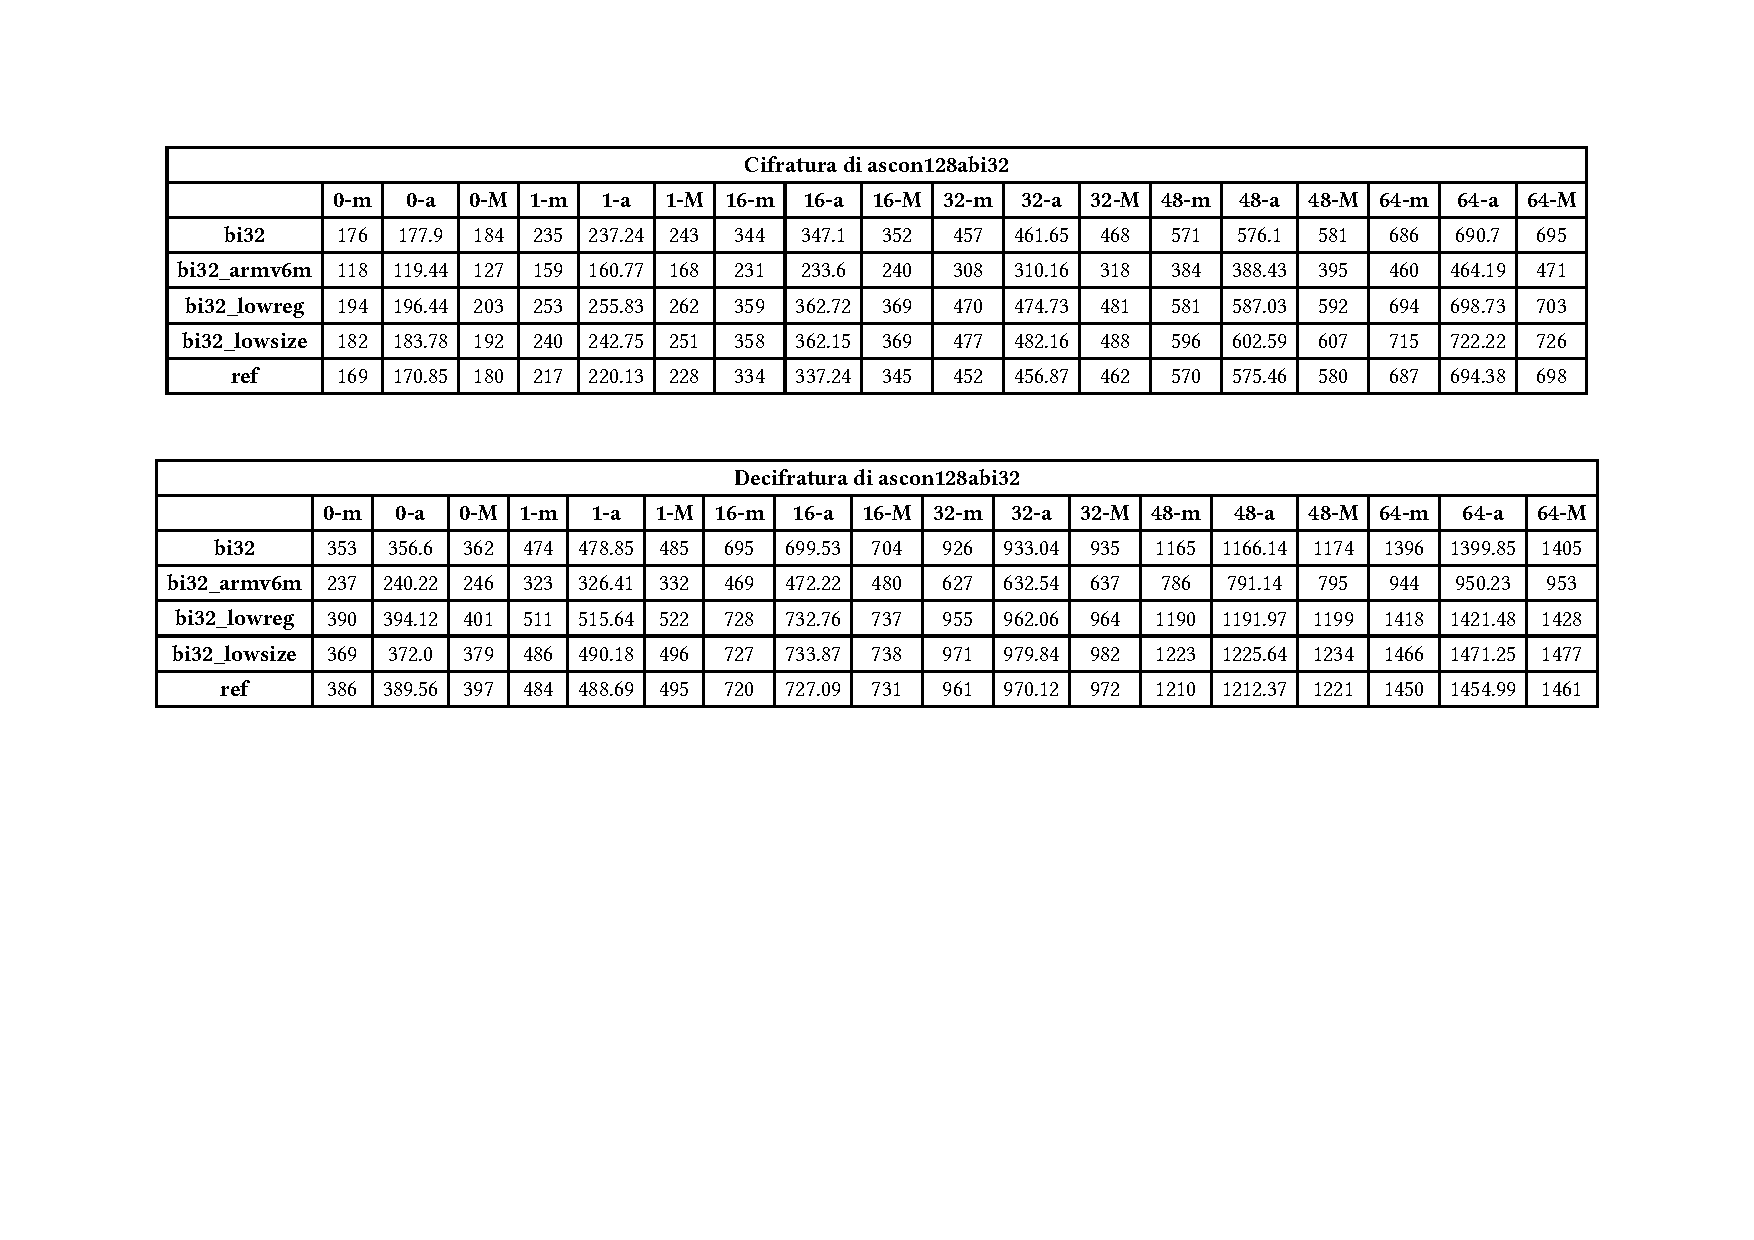
\includegraphics[width=0.6\textwidth]{adafruit/ascon128abi32.pdf}
    \caption{Plain-text di 0 byte con ascon128abi32.}
\end{figure}

\paragraph{Algoritmi no bi32}

In termini di tempi di esecuzione, l'implementazione armv6m si classifica prima in tutte le grandezze di plain-text, seguita da armv6m lowsize e bi32 armv6m, mentre le implementazioni bi32 lowreg e opt32 lowsize sono le peggiori. \\

\noindent Per quanto riguarda la dimensione dell'eseguibile, le implementazioni con lowsize nel nome sono risultate le migliori in tutte le grandezze di plain-text, seguite poco dopo dalla armv6m, confermando quindi la sua ottima posizione ottenuta nei tempi di esecuzione. Le implementazioni peggiori invece sono state la opt32 e la ref, con un'occupazione dello spazio circa il quadruplo dell'implementazione migliore.

\begin{figure}[H]
    \centering
    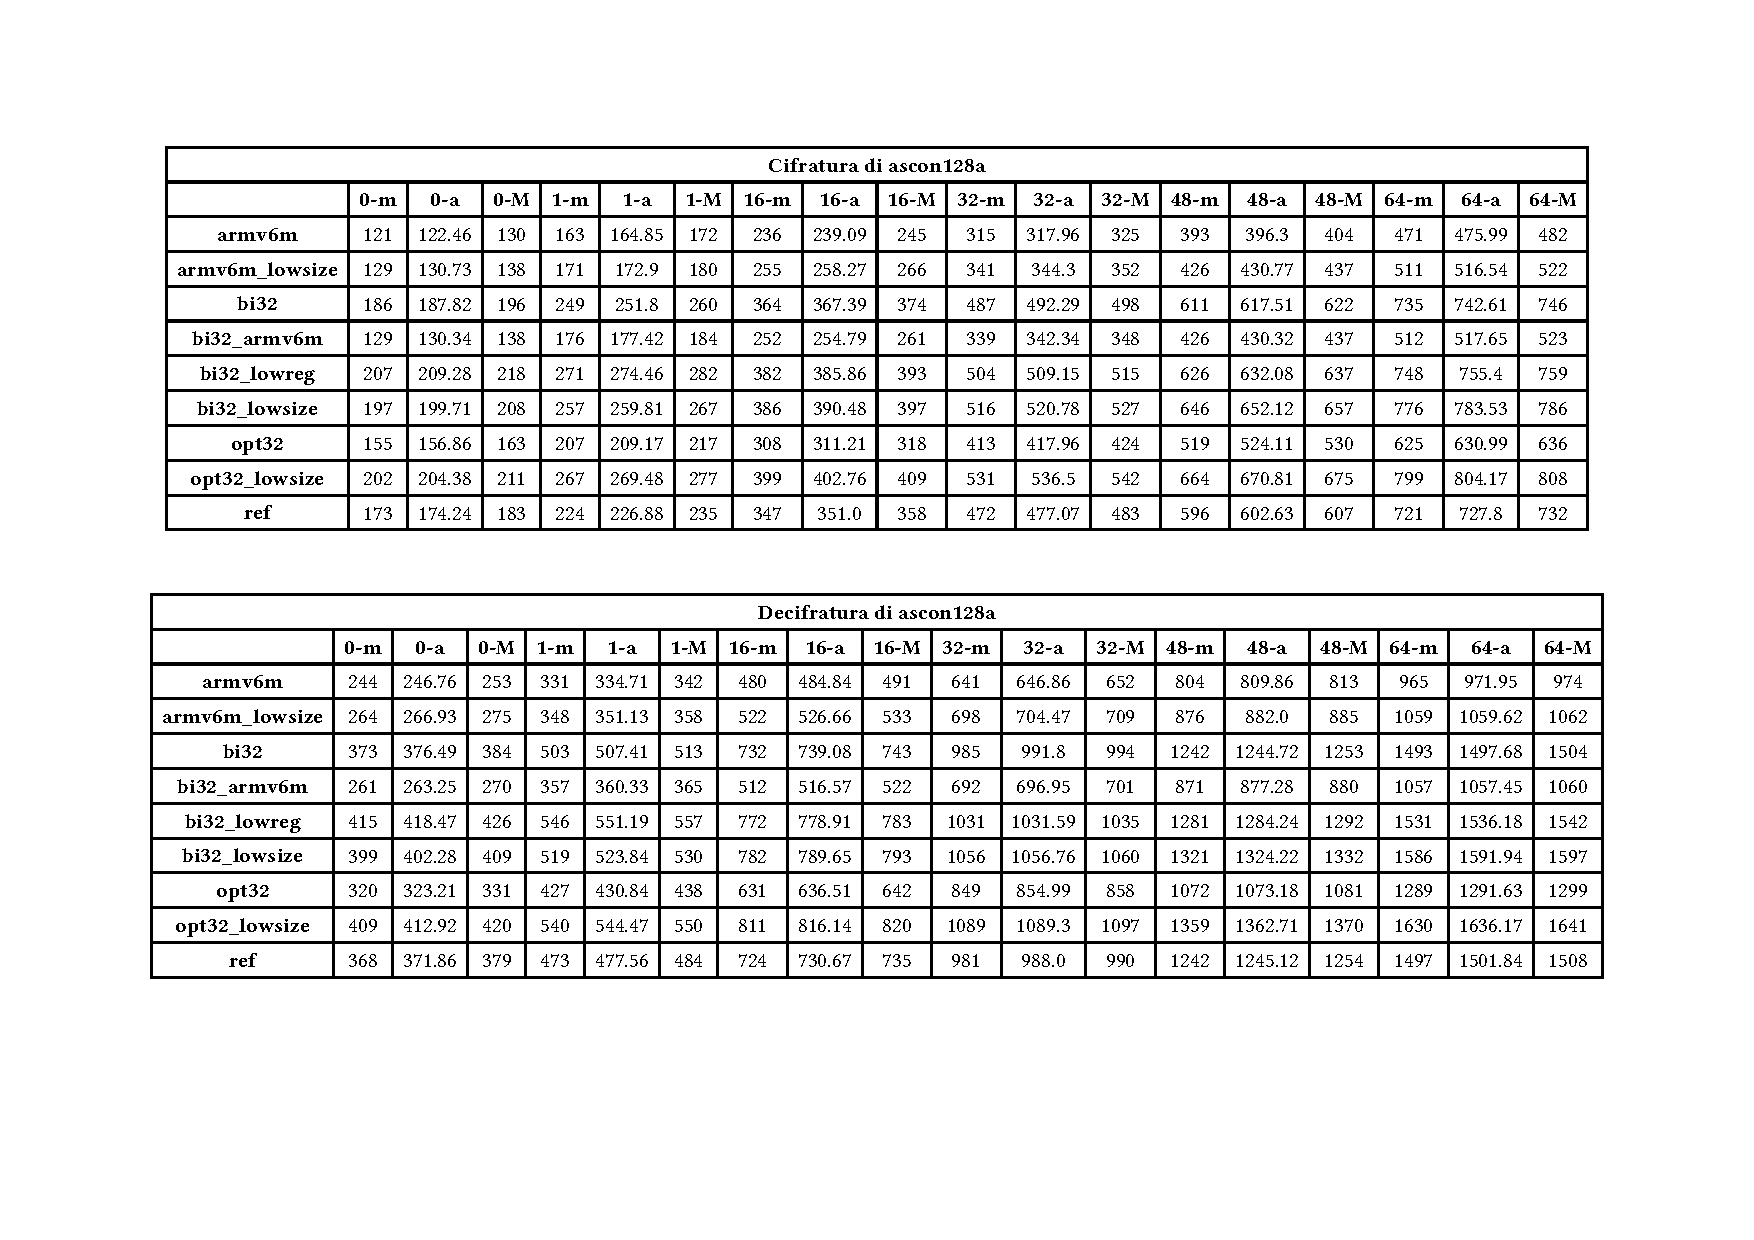
\includegraphics[width=0.6\textwidth]{adafruit/ascon128a.pdf}
    \caption{Plain-text di 0 byte con ascon128a.}
\end{figure}

\subsubsection{Crypto hash}

\paragraph{Algoritmi bi32}

In termini di tempi di esecuzione, l'implementazione bi32 armv6m è risultata la migliore in tutte le grandezze di plain-text, seguita a pari merito dalle altre implementazioni. Per plain-text fino a 64 byte, l'implementazione ref è stata la peggiore, mentre è diventata la seconda più veloce con plain-text più grandi, lasciando il primo posto come peggiore all'implementazione bi32 lowsize. \\

\noindent Per la dimensione dell'eseguibile, l'implementazione bi32 lowsize è risultata la migliore in tutte le grandezze di plain-text, seguita poco dopo dalla bi32 armv6m, confermando quindi la sua ottima posizione ottenuta nei tempi di esecuzione. L'implementazione peggiore invece è la ref, con una dimensione doppia rispetto a quella migliore.

\begin{figure}[H]
    \centering
    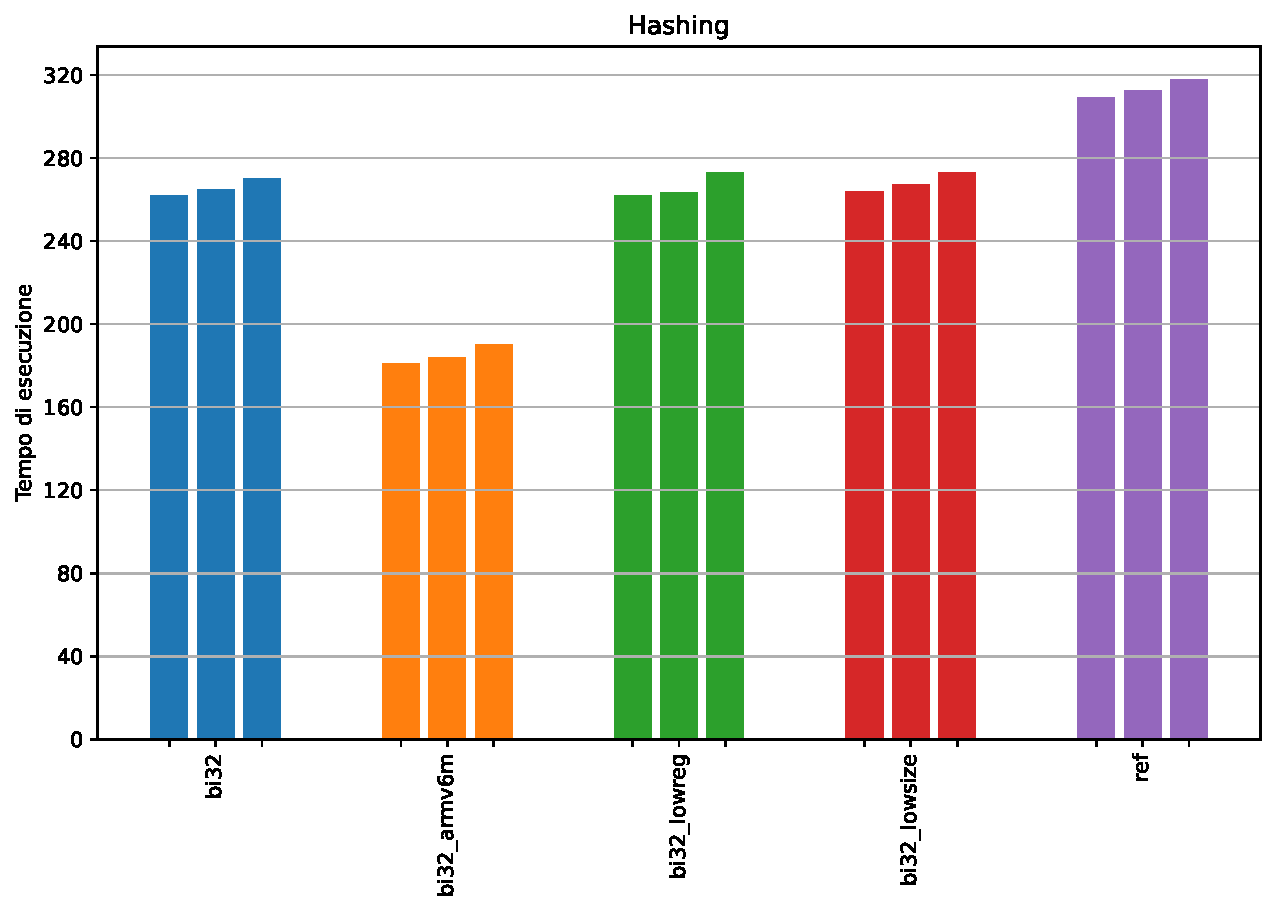
\includegraphics[width=0.6\textwidth]{adafruit/asconhashabi32.pdf}
    \caption{Plain-text di 0 byte con asconhashabi32.}
\end{figure}

\paragraph{Algoritmi no bi32}

In termini di tempi di esecuzione, l'implementazione armv6m è risultata la migliore in tutte le grandezze di plain-text, anche se le implementazioni armv6m lowsize e bi32 armv6m hanno tempi molto simili; le implementazioni opt32 lowsize e ref invece sono risultate le peggiori. \\

\noindent Come prima, nella la dimensione dell'eseguibile le implementazioni con lowsize nel nome sono risultate le migliori in tutte le grandezze di plain-text, seguite poco dopo dalla armv6m. L'implementazione peggiore invece è la ref, che si riconferma la peggiore implementazione: in questo caso ha occupato quasi il triplo dello spazio della migliore implementazione.

\begin{figure}[H]
    \centering
    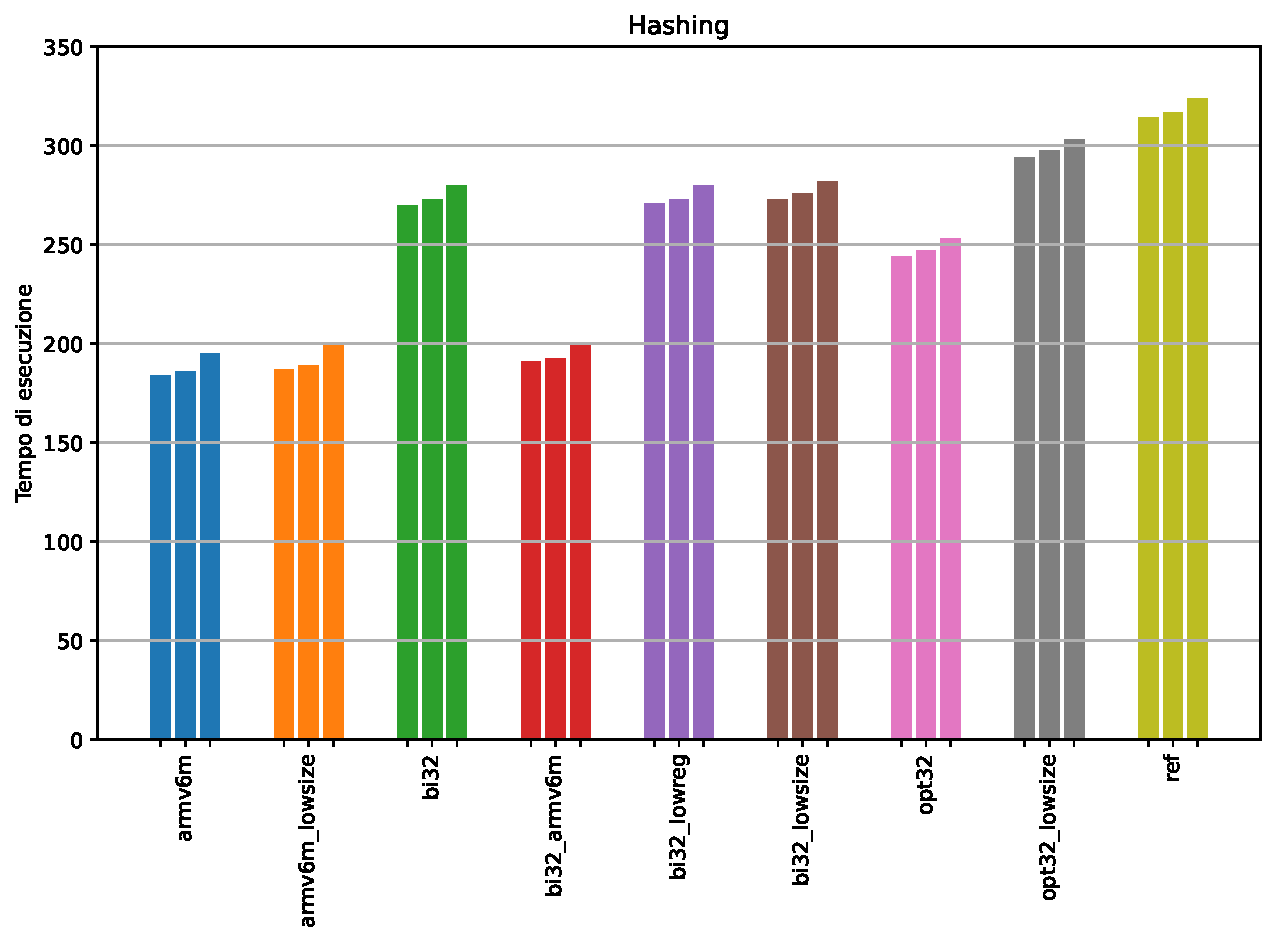
\includegraphics[width=0.6\textwidth]{adafruit/asconhasha.pdf}
    \caption{Plain-text di 0 byte con asconhasha.}
\end{figure}

\paragraph{Algoritmi XOF}

In termini di tempi di esecuzione, l'implementazione armv6m è risultata la migliore in tutte le grandezze di plain-text, seguita dalle implementazioni armv6m lowsize e bi32 armv6m, mentre le implementazioni opt32 lowsize e ref sono risultate le peggiori. \\

\noindent Osservando la dimensione dell'eseguibile, le implementazioni con lowsize nel nome sono risultate le migliori in tutte le grandezze di plain-text, seguite poco dopo dalla armv6m. L'implementazione peggiore invece è la ref, occupando quasi il triplo dello spazio che occupa l'implementazione migliore e confermando, come negli algoritmi no bi32, la sua posizione generale pessima.

\begin{figure}[H]
    \centering
    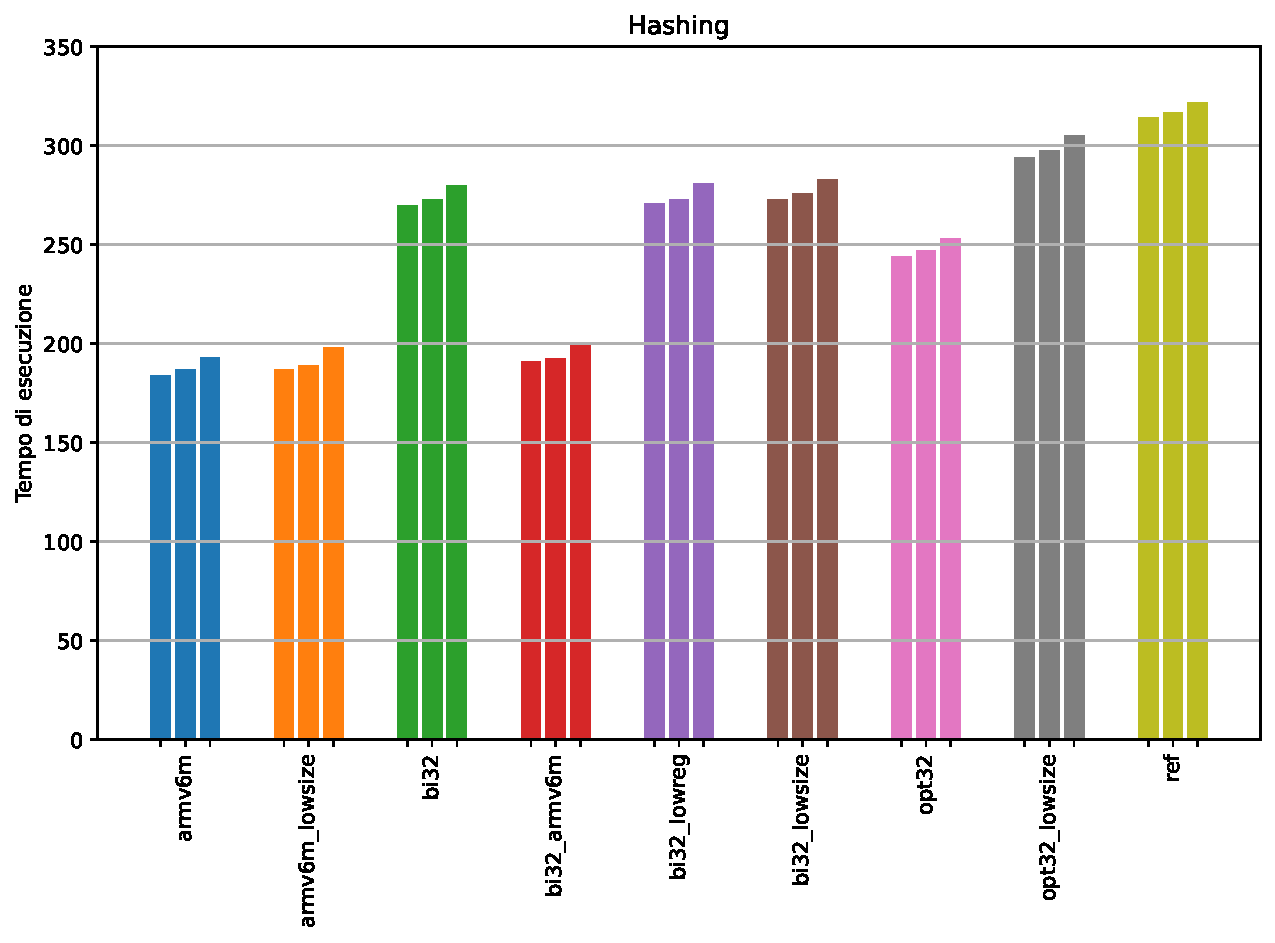
\includegraphics[width=0.6\textwidth]{adafruit/asconxofa.pdf}
    \caption{Plain-text di 0 byte con asconxofa.}
\end{figure}

\subsubsection{Crypto auth}

\paragraph{Algoritmi MAC}

In termini di tempi di esecuzione, l'implementazione armv6m è risultata la migliore in tutte le grandezze di plain-text, seguita dalle implementazioni bi32 armv6m e opt32, anche se quest'ultima è più lenta di circa il 21/27\% rispetto alla prima classificata se consideriamo l'algoritmo asconmaca; le implementazioni bi32, bi32 lowreg e ref si contendono invece i primi posti come peggiori. \\

\noindent Considerando la dimensione dell'eseguibile, l'implementazione armv6m è ancora la migliore, confermandosi come migliore implementazione in ogni aspetto, seguita dalle implementazioni bi32 armv6m e bi32 lowreg. Le implementazioni peggiori invece sono la opt32 e la ref, con una dimensione doppia rispetto a quella migliore.

\begin{figure}[H]
    \centering
    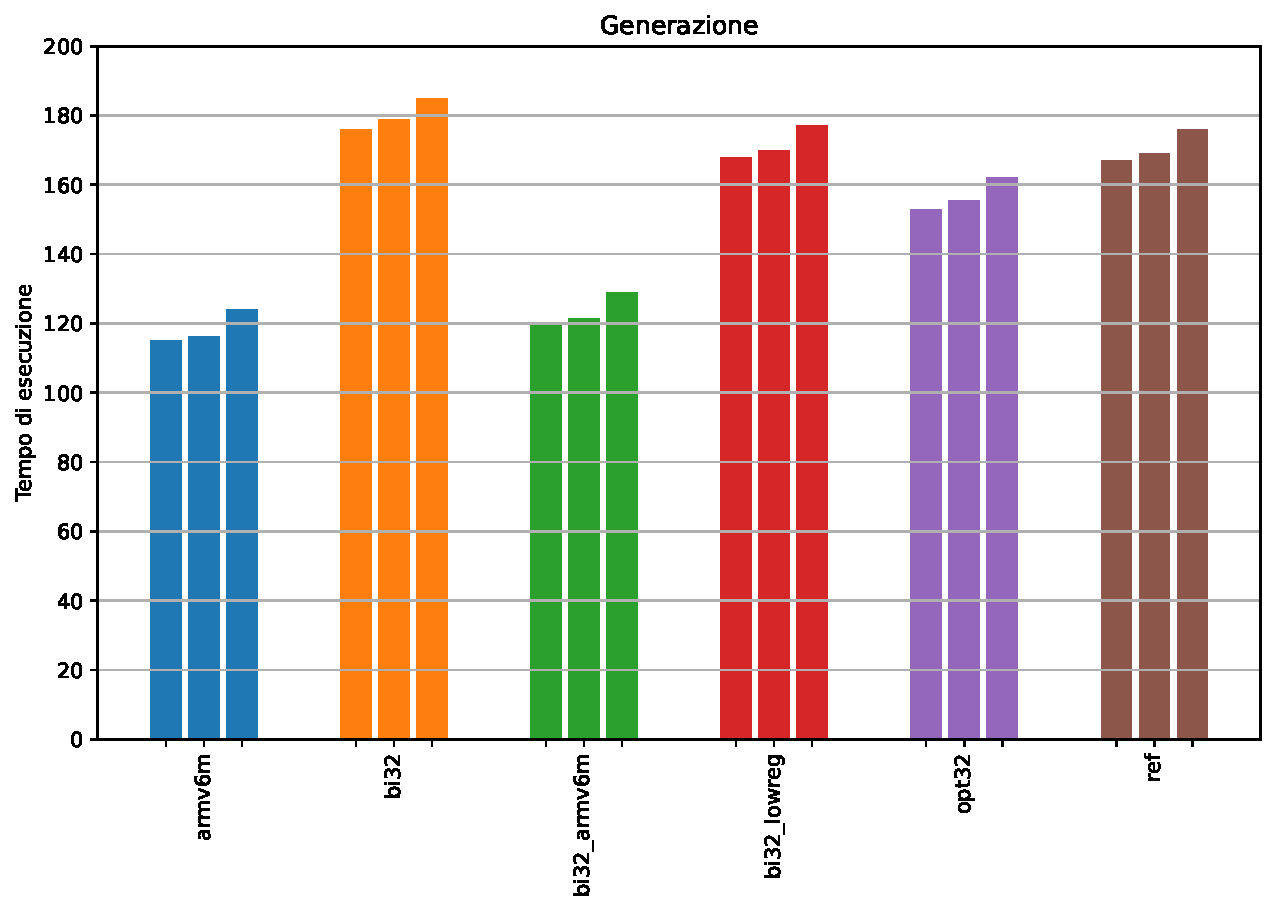
\includegraphics[width=0.6\textwidth]{adafruit/asconmaca.pdf}
    \caption{Plain-text di 0 byte con asconmaca.}
\end{figure}

\paragraph{Algoritmi PRF}

In termini di tempi di esecuzione, l'implementazione armv6m è risultata la migliore in tutte le grandezze di plain-text, seguita dalle implementazioni bi32 armv6m e opt32 hanno tempi molto simili, mentre le implementazioni bi32, bi32 lowreg e ref sono risultate le peggiori. \\

\noindent Osservando invece la dimensione dell'eseguibile, l'implementazione armv6m è ancora la migliore, confermandosi come migliore implementazione in ogni aspetto, seguita dalle implementazioni bi32 armv6m e bi32 lowreg. Le implementazioni peggiori invece sono la opt32 e la ref, con una dimensione doppia rispetto a quella migliore.

\begin{figure}[H]
    \centering
    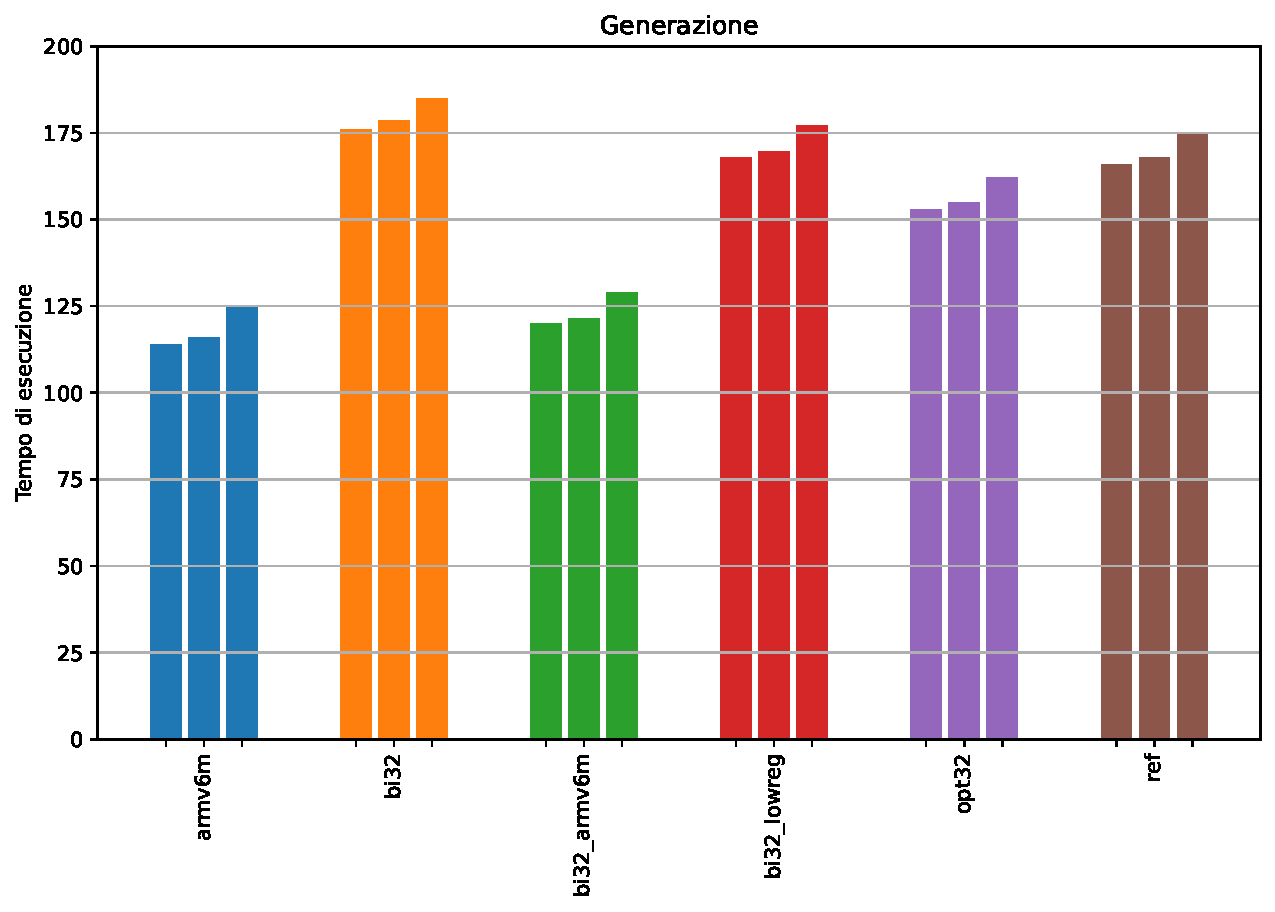
\includegraphics[width=0.6\textwidth]{adafruit/asconprfa.pdf}
    \caption{Plain-text di 0 byte con asconprfa.}
\end{figure}

\subsubsection{Recap finale}

Dalle analisi precedenti, possiamo quindi affermare che le implementazioni armv6m e bi32 armv6m sono risultate le migliori in ogni algoritmo considerato, mentre alcune implementazioni che avevano dei flag di ottimizzazione specifici, come ad esempio le implementazioni bi32, si sono comportate peggio di quelle prive di flag.

\subsection{Arduino Due}

\subsubsection{Crypto AEAD}

\paragraph{Algoritmi bi32}

In termini di tempi di esecuzione, l'implementazione bi32 armv7m è risultata la migliore in tutte le grandezze di plain-text, seguita dalle implementazioni bi32 generiche, mentre l'implementazione ref è risultata la peggiore: infatti, risulta quasi tre volte più lenta della seconda peggiore e poco meno di dieci volte più lenta di quella migliore. \\

\noindent Nello studio della dimensione dell'eseguibile l'implementazione bi32 lowsize è risultata la migliore in tutte le grandezze di plain-text, seguita dalla ref, che si riprende dopo la pessima posizione ottenuta nei tempi di esecuzione. L'implementazione peggiore invece è la bi32 armv7m, che invece era la migliore nei tempi di esecuzione.

\begin{figure}[H]
    \centering
    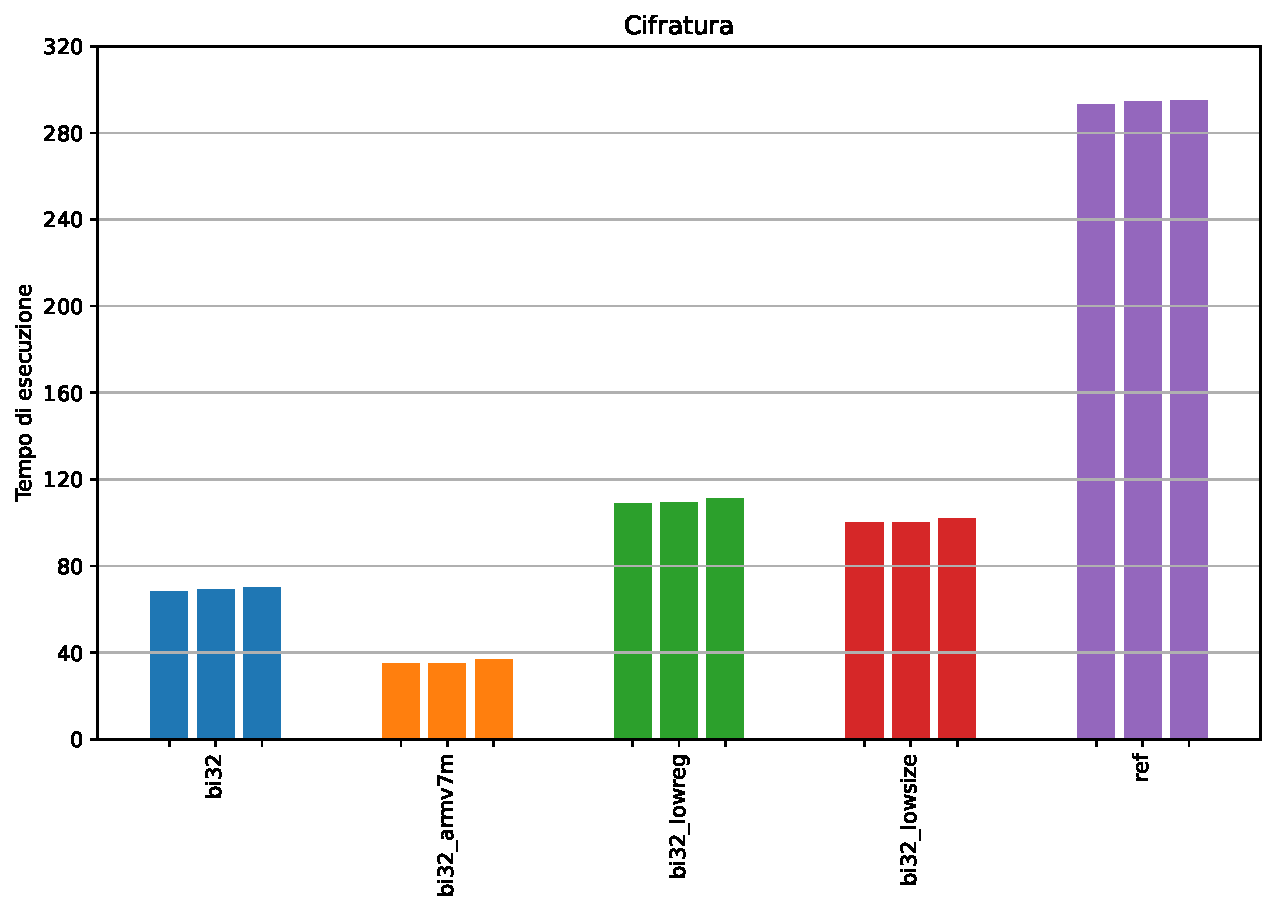
\includegraphics[width=0.6\textwidth]{arduino/ascon128abi32.pdf}
    \caption{Plain-text di 0 byte con ascon128abi32.}
\end{figure}

\paragraph{Algoritmi no bi32}

In termini di tempi di esecuzione, l'implementazione armv7m small è risultata la migliore in tutte le grandezze di plain-text, seguita dalle implementazioni bi32 armv7m, armv7m lowsize e armv7m, mentre l'implementazione ref è risultata la peggiore di quasi quattro volte rispetto alla migliore. \\

\noindent Per quanto riguarda la dimensione dell'eseguibile, le implementazioni con lowsize e small nel nome sono risultate le migliori in tutte le grandezze di plain-text, seguite dalla ref, che si riprende dopo la pessima posizione ottenuta nei tempi di esecuzione, e dalla armv7m small, che si dimostra quindi un'ottima soluzione anche per lo spazio occupato. L'implementazione peggiore invece è la ref, occupando quasi il quadruplo dello spazio che occupa l'implementazione migliore.

\begin{figure}[H]
    \centering
    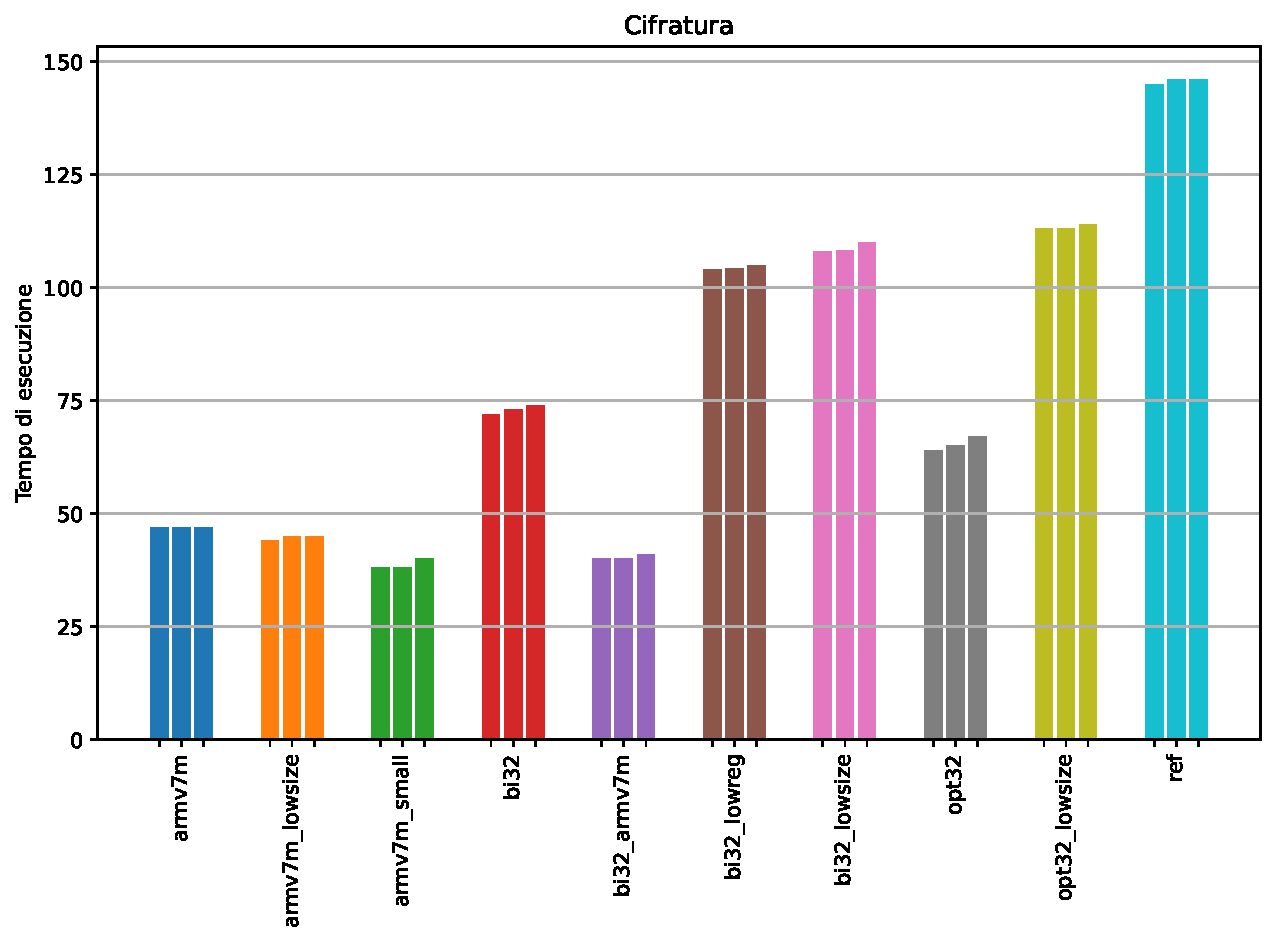
\includegraphics[width=0.6\textwidth]{arduino/ascon128a.pdf}
    \caption{Plain-text di 0 byte con ascon128a.}
\end{figure}

\subsubsection{Crypto hash}

\paragraph{Algoritmi bi32}

In termini di tempi di esecuzione, l'implementazione bi32 armv7m è risultata la migliore in tutte le grandezze di plain-text, seguita dalle altre implementazioni bi32. L'implementazione ref è invece la peggiore, che è oltre tre volte più lenta della seconda peggiore e dieci volte più lenta di quella migliore. \\

\noindent Per la dimensione dell'eseguibile, l'implementazione bi32 lowsize è risultata la migliore in tutte le grandezze di plain-text, seguita dalla ref, che si riprende dopo la pessima posizione nei tempi di esecuzione. Le implementazioni peggiori sono invece la bi32 armv7m, che tuttavia compensa con il migliore tempo di esecuzione, e la bi32.

\begin{figure}[H]
    \centering
    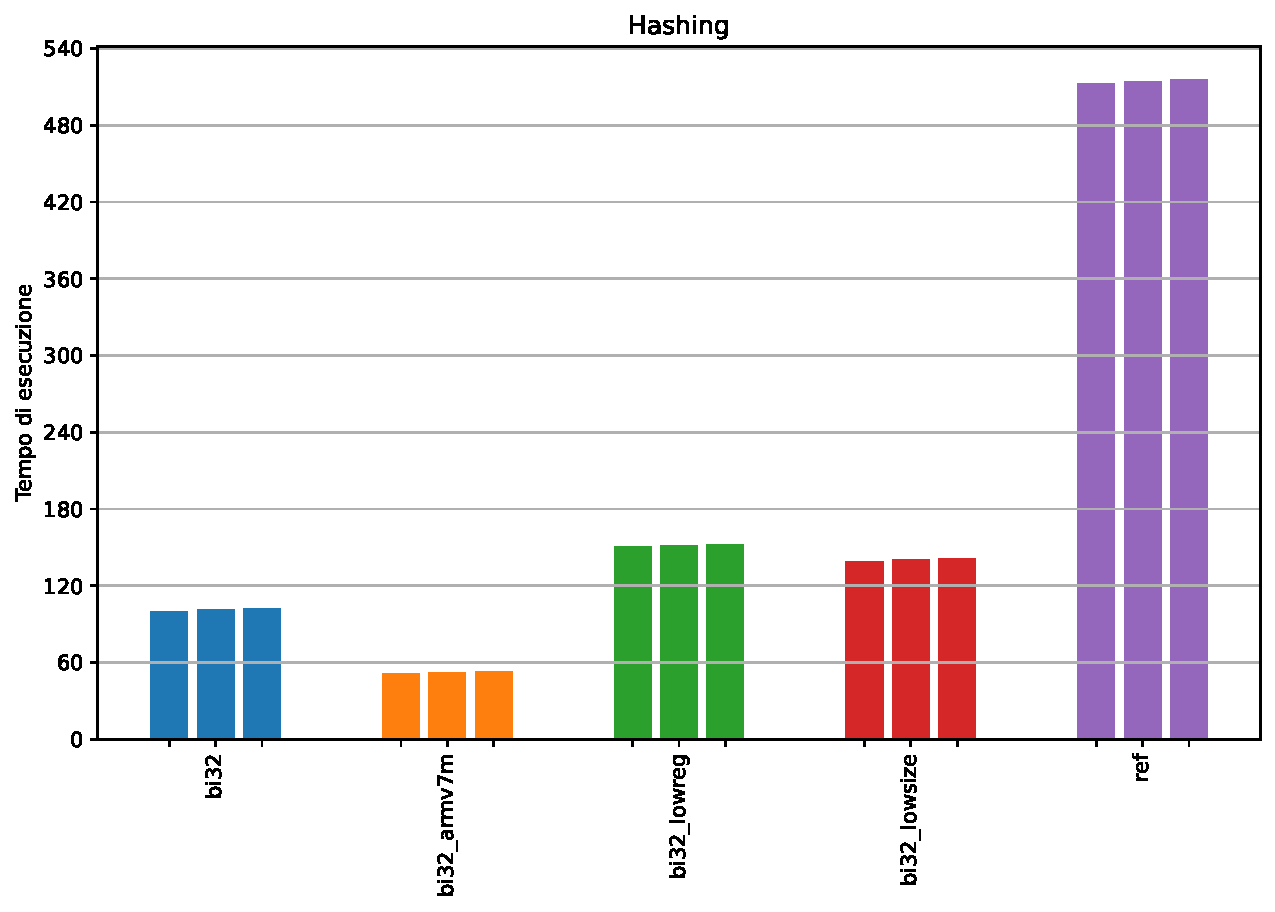
\includegraphics[width=0.6\textwidth]{arduino/asconhashabi32.pdf}
    \caption{Plain-text di 0 byte con asconhashabi32.}
\end{figure}

\paragraph{Algoritmi no bi32}

In termini di tempi di esecuzione, le implementazioni bi32 armv7m, armv7m small e armv7m lowsize sono risultate le migliori, con la bi32 armv7m che diventa la migliore se la grandezza dei plain-text aumenta, mentre le implementazioni della famiglia opt32 e ref sono risultate le peggiori, anche se quest'ultima è più lenta del 23/27\% rispetto alle altre. \\

\noindent Oltre alla classica lowsize, nella dimensione dell'eseguibile le implementazioni con lowreg e small nel nome sono risultate le migliori in tutte le grandezze di plain-text, seguite poco dopo dalla bi32 armv7m, confermando quindi la sua ottima posizione ottenuta nei tempi di esecuzione, e dalla ref, che recupera parzialmente la pessima posizione nei tempi di esecuzione. L'implementazione peggiore invece è la opt32, la quale occupa quasi il triplo dello spazio dell'implementazione migliore.

\begin{figure}[H]
    \centering
    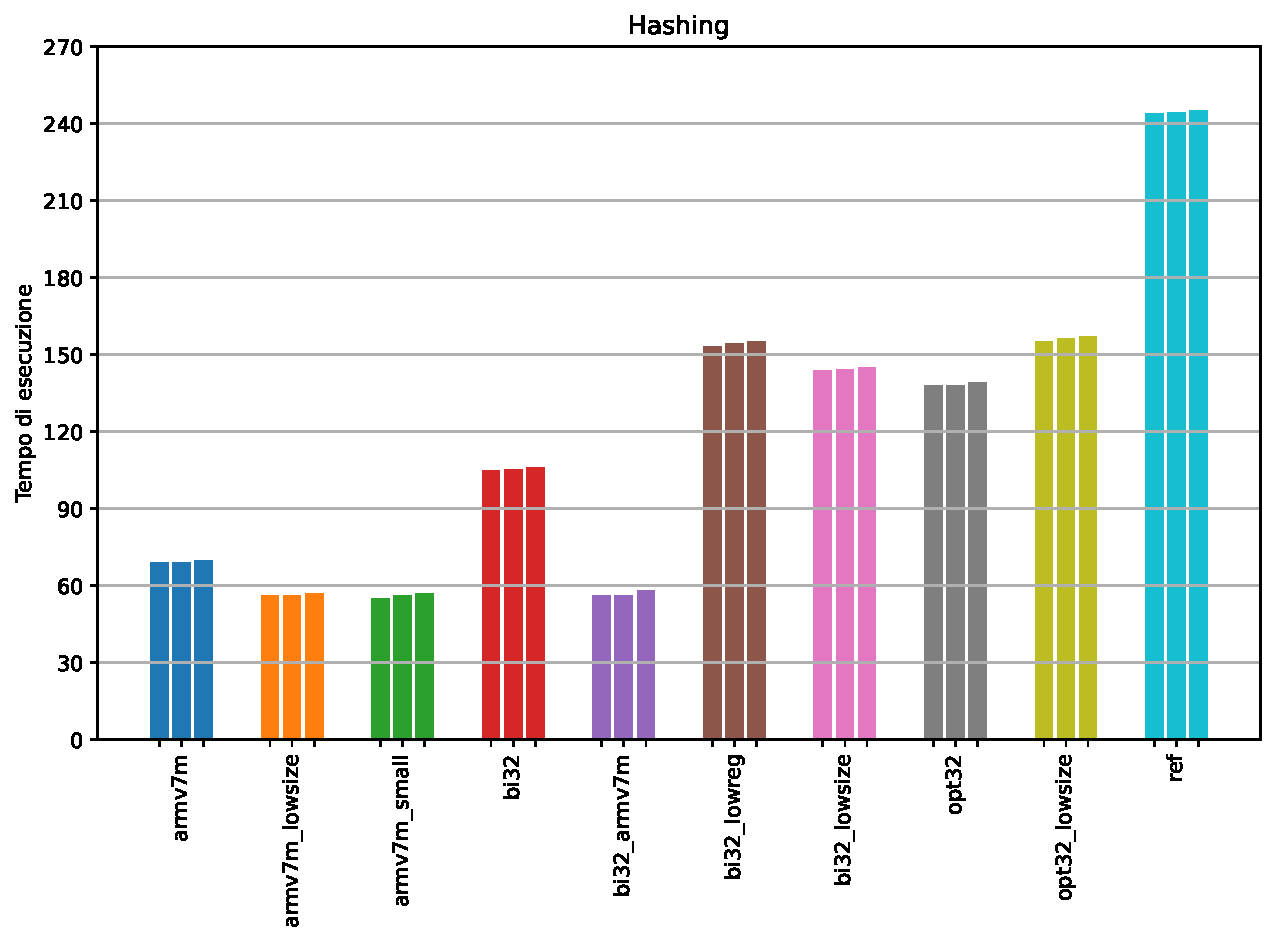
\includegraphics[width=0.6\textwidth]{arduino/asconhasha.pdf}
    \caption{Plain-text di 0 byte con asconhasha.}
\end{figure}

\paragraph{Algoritmi XOF}

In termini di tempi di esecuzione, le implementazioni bi32 armv7m, armv7m small e armv7m lowsize sono risultate le migliori, con la bi32 armv7m che diventa la migliore se la grandezza dei plain-text aumenta, mentre le implementazioni della famiglia opt32 e ref sono risultate le peggiori, anche se quest'ultima è molto più lenta del 24/27\% rispetto alle altre. \\

\noindent Come prima, per la dimensione dell'eseguibile le implementazioni con lowsize, lowreg e small nel nome sono risultate le migliori in tutte le grandezze di plain-text, seguite poco dopo dalla bi32 armv7m, confermando quindi la sua ottima posizione ottenuta nei tempi di esecuzione, e dalla ref, che recupera parzialmente la pessima posizione nei tempi di esecuzione. L'implementazione peggiore invece è la opt32, il triplo più pesante dell'implementazione migliore.

\begin{figure}[H]
    \centering
    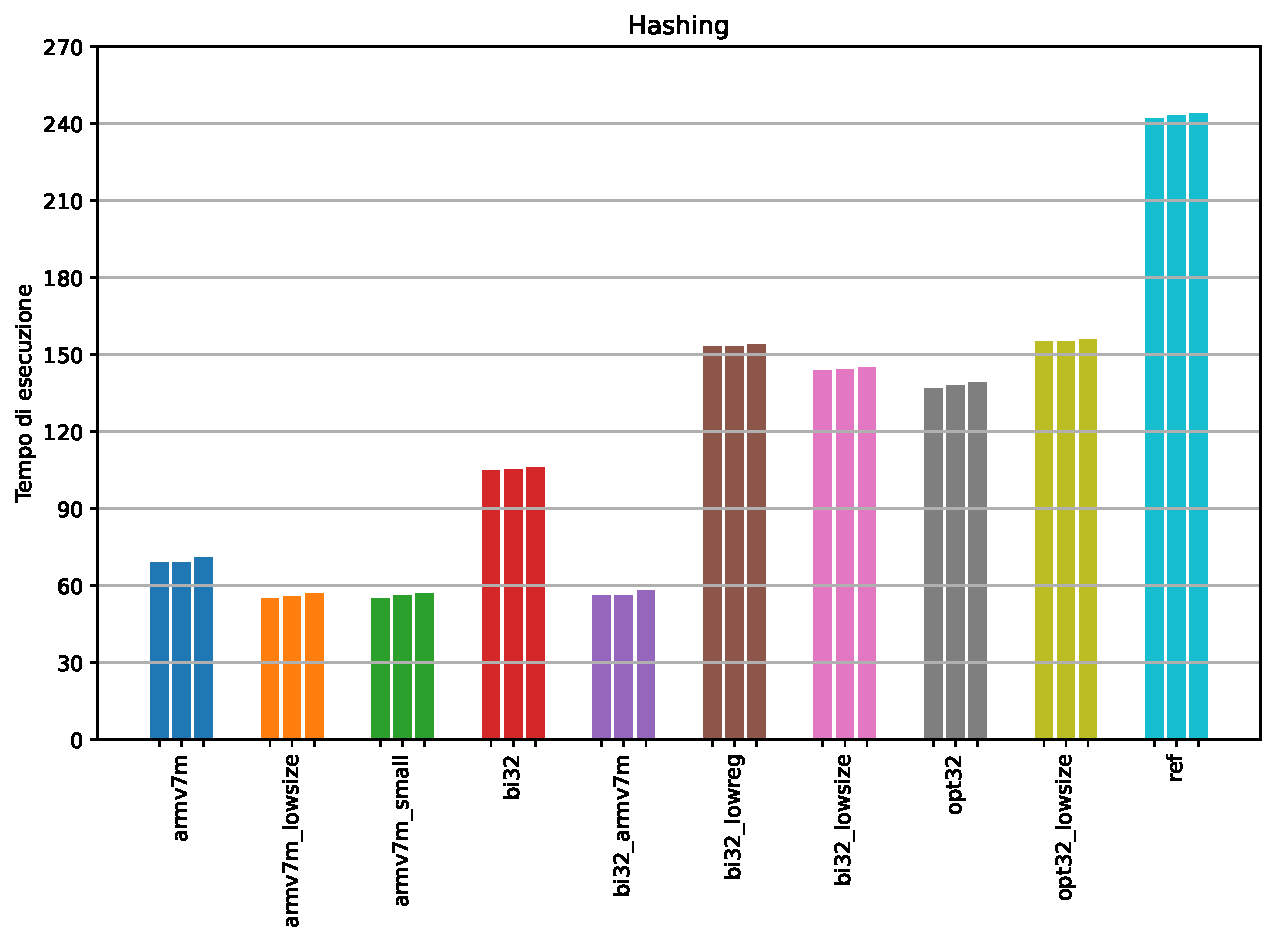
\includegraphics[width=0.6\textwidth]{arduino/asconxofa.pdf}
    \caption{Plain-text di 0 byte con asconxofa.}
\end{figure}

\subsubsection{Crypto auth}

\paragraph{Algoritmi MAC}

In termini di tempi di esecuzione, le implementazioni bi32 armv7m, armv7m small e armv7m si contendono le prime tre posizioni al variare delle grandezze di plain-text, mentre l'implementazione ref è la peggiore. \\

\noindent Considerando la dimensione dell'eseguibile, le implementazioni armv7m small, ref e bi32 lowreg sono le migliori, ma solo la prima può vantare anche ottimi tempi di esecuzione. L'implementazione peggiore invece è la opt32, con una dimensione doppia rispetto a quella migliore.

\begin{figure}[H]
    \centering
    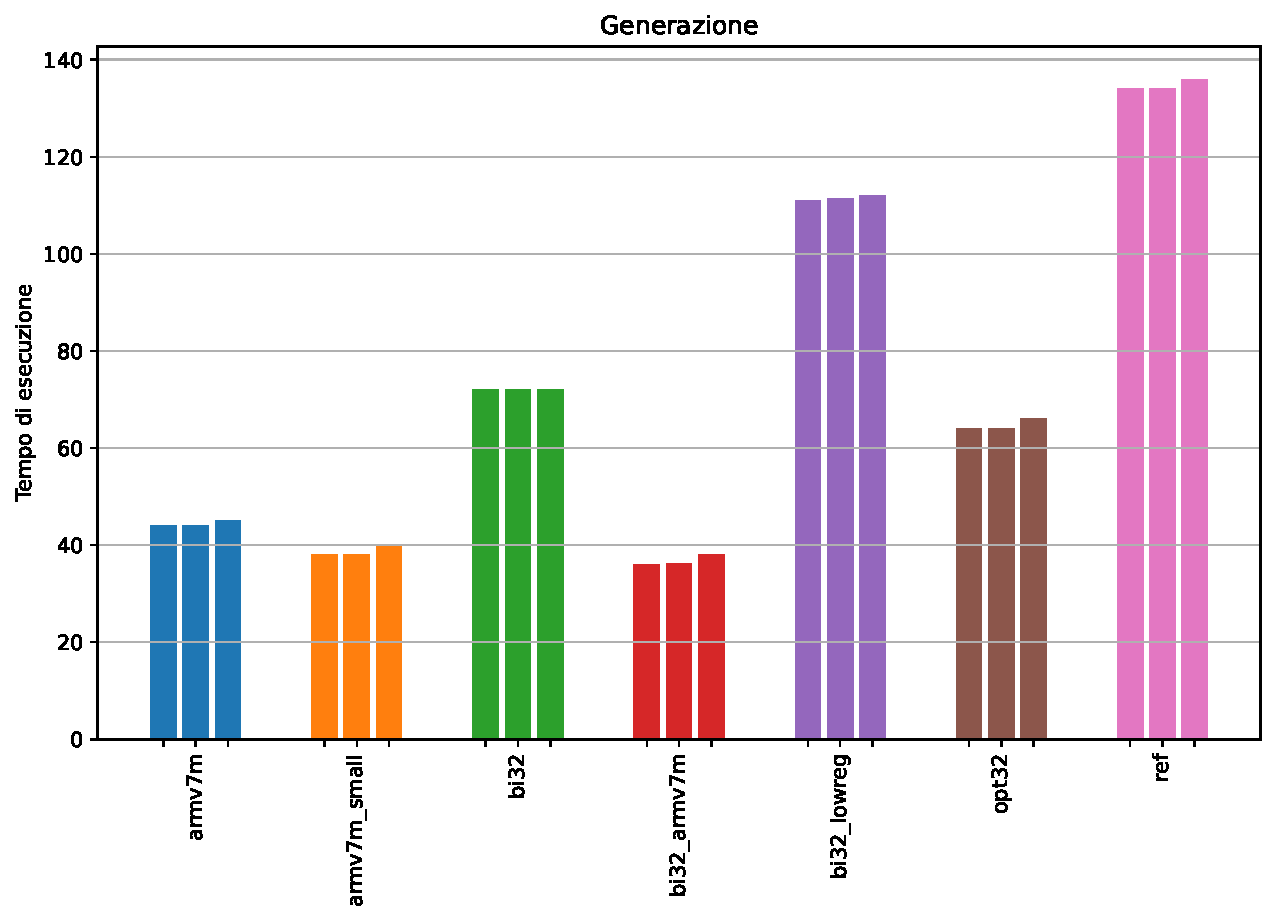
\includegraphics[width=0.6\textwidth]{arduino/asconmaca.pdf}
    \caption{Plain-text di 0 byte con asconmaca.}
\end{figure}

\paragraph{Algoritmi PRF}

In termini di tempi di esecuzione, le implementazioni armv7m small e bi32 armv7m sono risultate le migliori in tutte le grandezze di plain-text, con la prima che è più performante su plain-text di grandezza maggiore, mentre l'implementazione ref è risultata la peggiore. \\

\noindent Per la dimensione dell'eseguibile, le implementazioni armv7m small, ref e bi32 lowreg sono le migliori, ma solo la prima può  anche ottimi tempi di esecuzione. L'implementazione peggiore invece è la opt32, con una dimensione quasi tripla rispetto a quella migliore.

\begin{figure}[H]
    \centering
    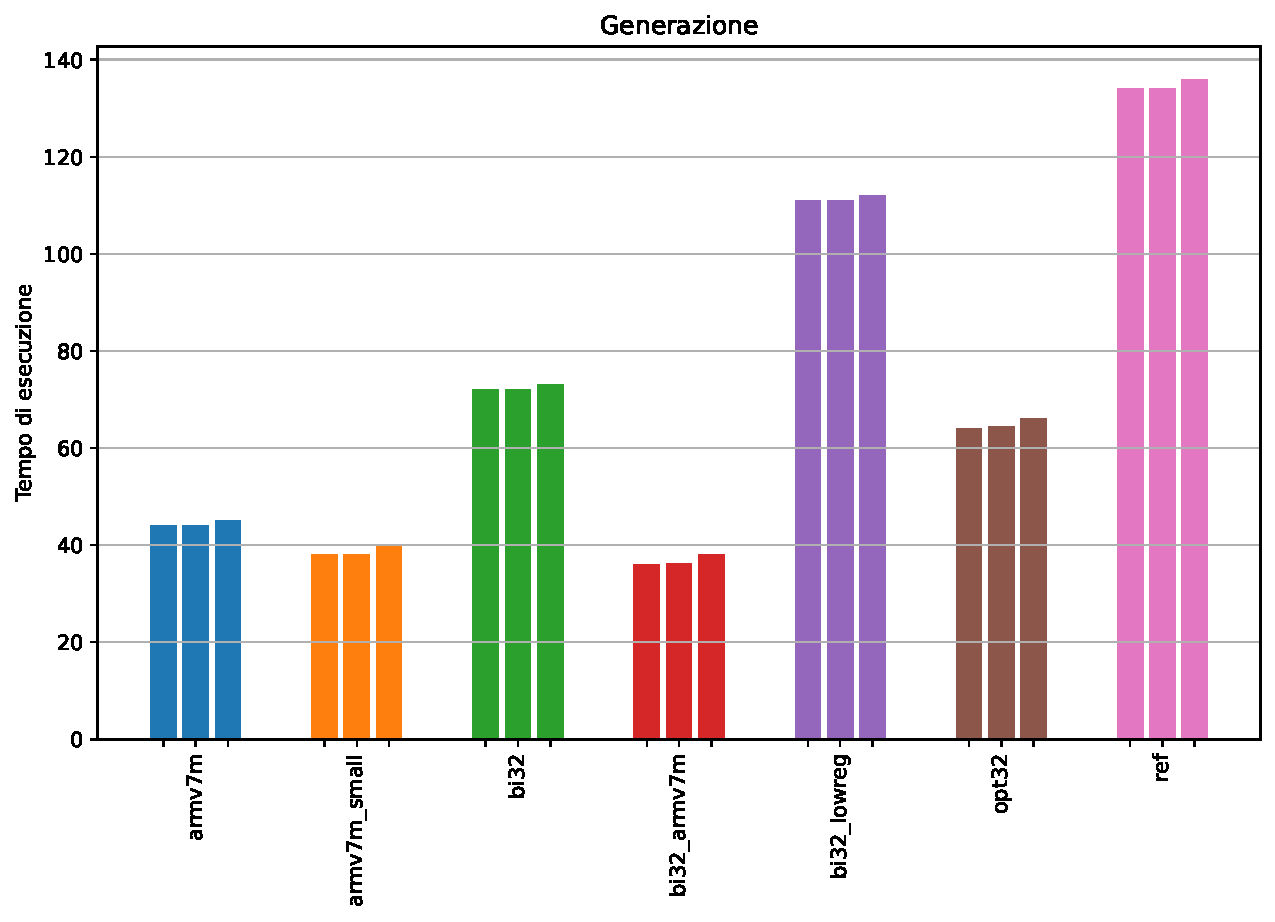
\includegraphics[width=0.6\textwidth]{arduino/asconprfa.pdf}
    \caption{Plain-text di 0 byte con asconprfa.}
\end{figure}

\subsubsection{Recap finale}

Dalle analisi precedenti, possiamo affermare che le implementazioni bi32 armv7m e armv7m small sono risultate le migliori in ogni algoritmo considerato, mentre l'implementazione ref si è trovata spesso tra le peggiori implementazioni.

\subsection{RaspberryPi model 3B}

Come specificato all'inizio di questo capitolo, i dati per questa board sono influenzati dalla velocità di esecuzione sotto il microsecondo e dalla presenza dello scheduler del sistema operativo. Inoltre, non saranno presenti gli algoritmi bi32 perchè la board possiede un'architettura 64 bit, che non rientra nelle ottimizzazioni fornite da ASCON.

\subsubsection{Crypto AEAD}

\paragraph{Algoritmi classici}

In termini di tempi di esecuzione, nessuna implementazione riesce a dominare definitivamente le altre, mentre per la dimensione dell'eseguibile l'implementazione opt64 lowsize è risultata la migliore, seguita dalla ref e dalla opt64, che hanno praticamente la stessa grandezza.

\begin{figure}[H]
    \centering
    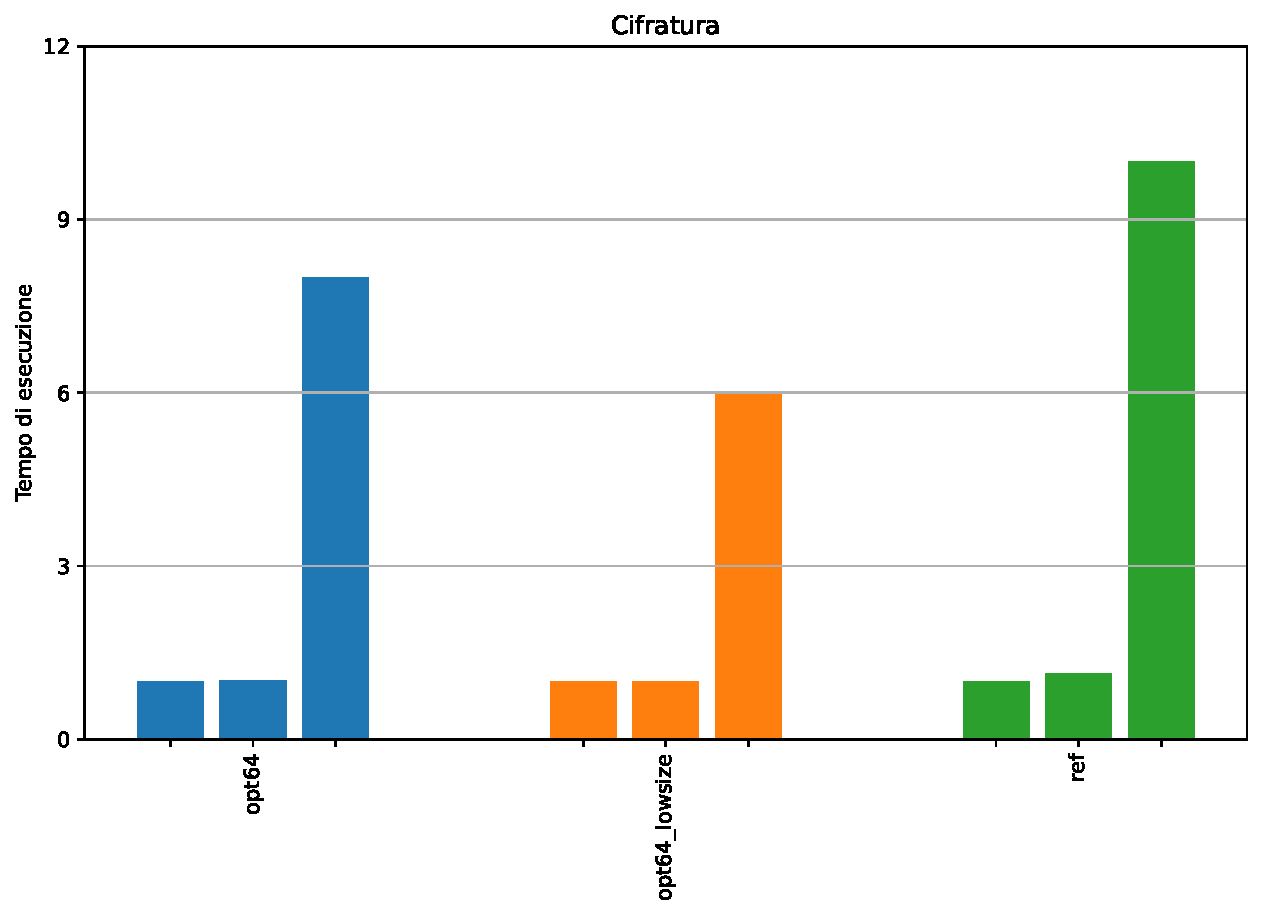
\includegraphics[width=0.6\textwidth]{raspberry/ascon128a.pdf}
    \caption{Plain-text di 0 byte con ascon128a.}
\end{figure}

\subsubsection{Crypto hash}

\paragraph{Algoritmi hash}

In termini di tempi di esecuzione, per grandezze di plain-text ridotte nessuna implementazione riesce a dominare definitivamente le altre, mentre le restanti grandezze opt64 diventa la migliore e opt64 lowsize la peggiore.

\noindent Considerando invece la dimensione dell'eseguibile, l'implementazione opt64 lowsize è risultata la migliore, seguita dalla ref e dalla opt64, anche se i due valori differiscono di un numero di byte compreso tra 40 e 88.

\begin{figure}[H]
    \centering
    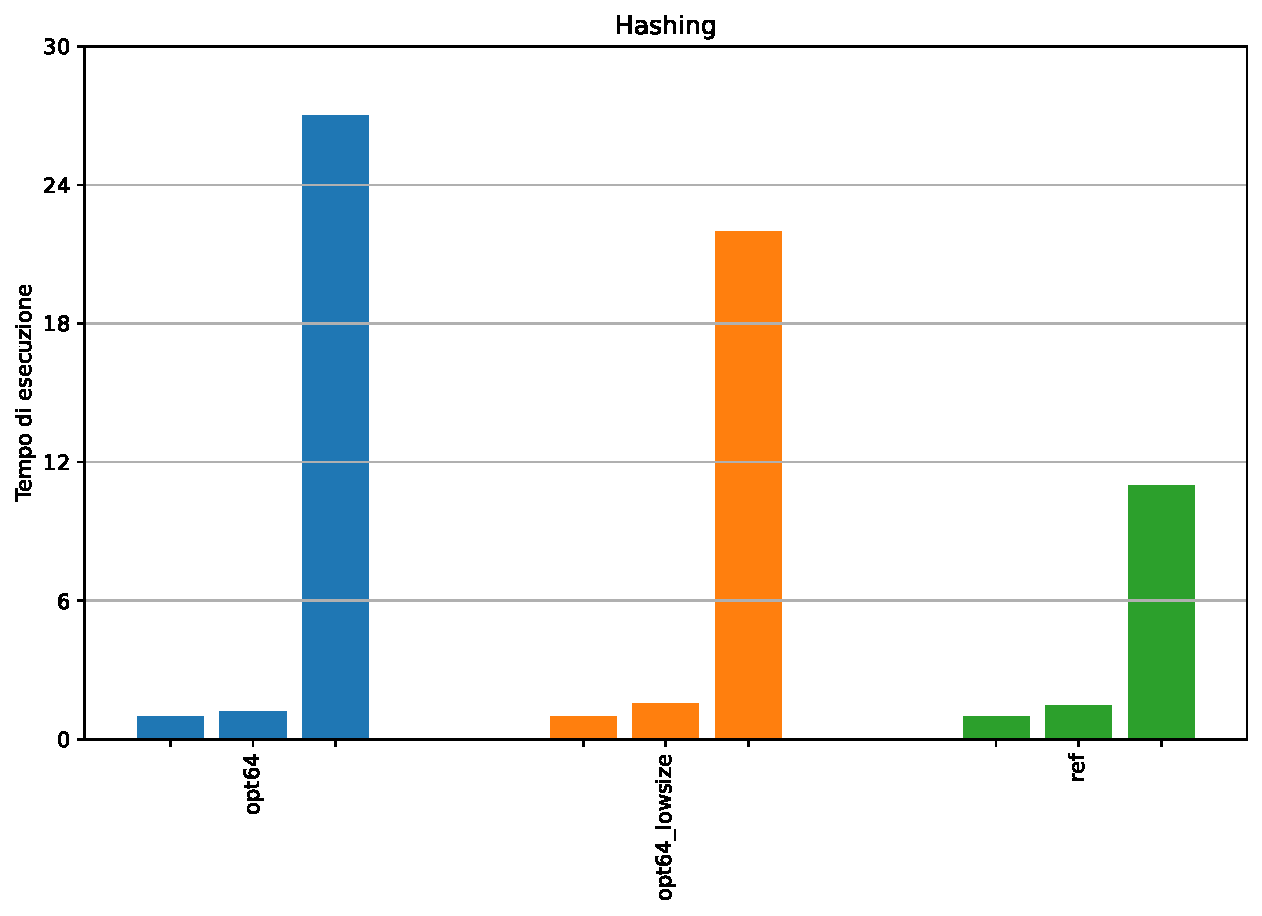
\includegraphics[width=0.6\textwidth]{raspberry/asconhasha.pdf}
    \caption{Plain-text di 0 byte con asconhasha.}
\end{figure}

\paragraph{Algoritmi XOF}

In termini di tempi di esecuzione, per grandezze di plain-text ridotte nessuna implementazione riesce a dominare definitivamente le altre, mentre per grandezze maggiori opt64 diventa la migliore e opt64 lowsize diventa la peggiore.

\noindent Per la dimensione dell'eseguibile, l'implementazione opt64 lowsize è risultata la migliore, seguita dalla ref e dalla opt64, anche se, come prima, i due valori differiscono di un numero di byte compreso tra 40 e 88.

\begin{figure}[H]
    \centering
    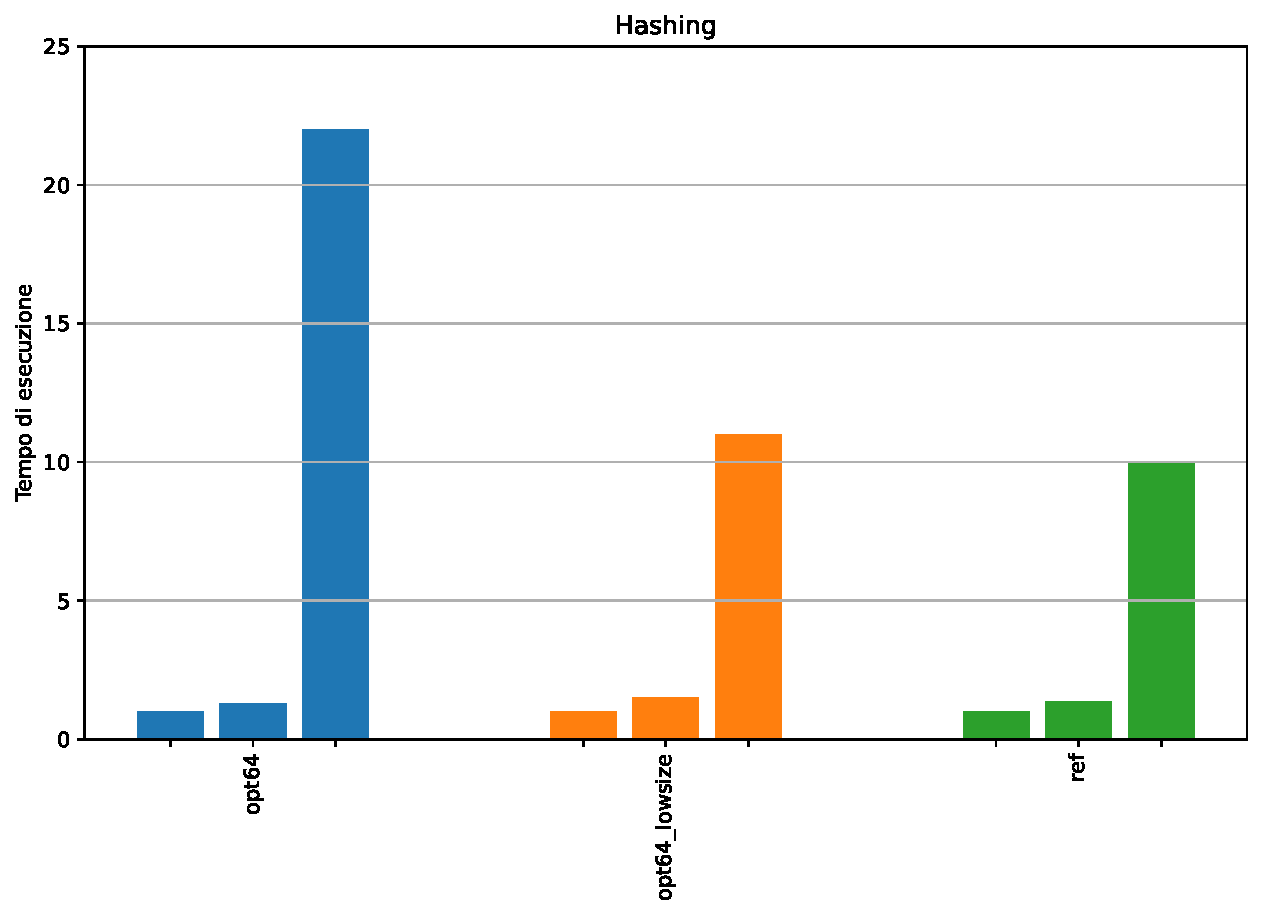
\includegraphics[width=0.6\textwidth]{raspberry/asconxofa.pdf}
    \caption{Plain-text di 0 byte con asconxofa.}
\end{figure}

\subsubsection{Crypto auth}

\paragraph{Algoritmi MAC}

In termini di tempi di esecuzione, per grandezze di plain-text ridotte nessuna implementazione riesce a dominare definitivamente le altre, mentre per grandezze maggiori opt64 diventa la migliore e ref diventa la peggiore. \\

\noindent Nello studio della dimensione dell'eseguibile, l'implementazione ref è risultata la migliore, seguita dalla opt64, che si classifica ultima, anche se i due valori differiscono di un numero di byte compreso tra 24 e 48, quindi le possiamo considerare praticamente allo stesso livello.

\begin{figure}[H]
    \centering
    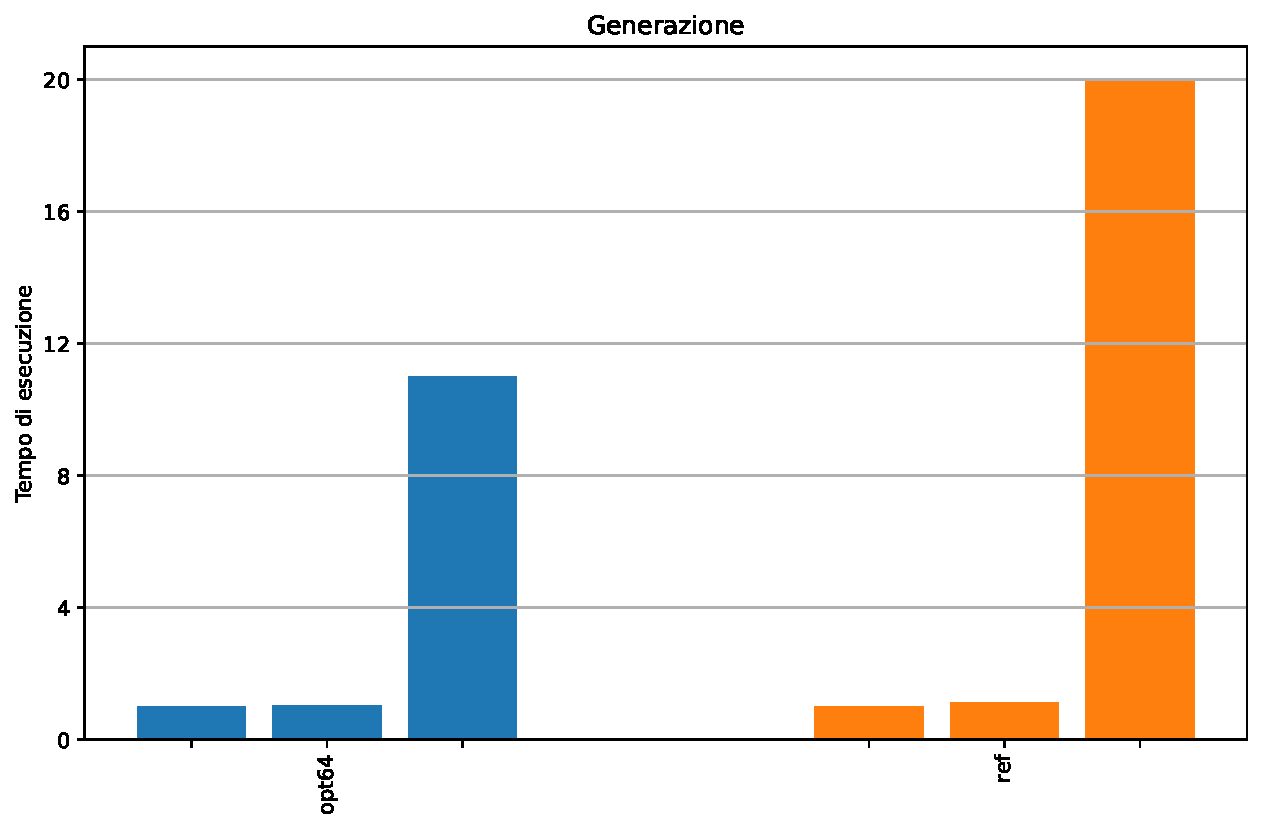
\includegraphics[width=0.6\textwidth]{raspberry/asconmaca.pdf}
    \caption{Plain-text di 0 byte con asconmaca.}
\end{figure}

\paragraph{Algoritmi PRF}

In termini di tempi di esecuzione, nessuna implementazione riesce a dominare definitivamente l'altra. \\

\noindent Considerando invece la dimensione dell'eseguibile, l'implementazione ref  è risultata la migliore, seguita dalla opt64, che si classifica ultima, anche se i due valori differiscono di un numero di byte compreso tra 24 e 48, quindi sono da considerarsi allo stesso livello.

\begin{figure}[H]
    \centering
    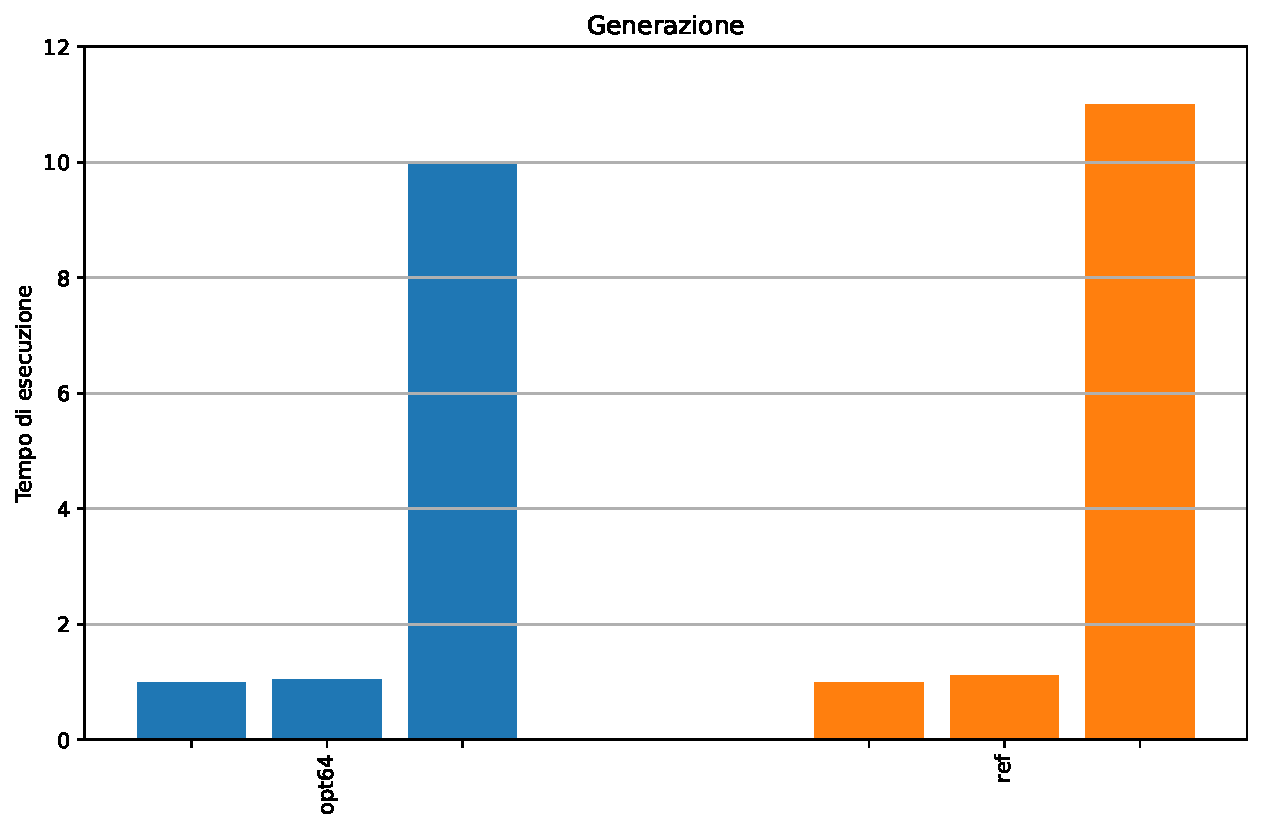
\includegraphics[width=0.6\textwidth]{raspberry/asconprfa.pdf}
    \caption{Plain-text di 0 byte con asconprfa.}
\end{figure}

\subsubsection{Recap finale}

A differenze delle board precedenti, il pool di implementazioni disponibili è molto ridotto, formato infatti dalle sole implementazioni opt64, opt64 lowsize e ref. Dalle analisi precedenti, l'implementazione opt64 è la migliore per quanto riguarda i tempi di esecuzione, soprattutto su plain-text di grandezza maggiore. Se l'ottimizzazione va invece verso lo spazio utilizzato, permettendo alcune perdite in termini di tempo di esecuzione, soprattutto sui plain-text di grandezza maggiore l'implementazione opt64 lowsize è la scelta migliore. L'implementazione ref è nel mezzo e non ha senso considerarla, perchè: \begin{itemize}
    \item se l'ottimizzazione va verso i tempi di esecuzione, ref è più lenta della opt64 ma con lo stesso spazio utilizzato;
    \item se l'ottimizzazione va verso lo spazio utilizzato, ref è più pesante della opt64 lowsize ma con dei tempi di esecuzione molto simili.
\end{itemize}

\newpage

\chapter{Conclusioni}

1 pagina dove termino il discorso

\newpage

\printbibliography

\end{document}
